\documentclass{article}

\usepackage[T1]{fontenc}
\usepackage[utf8]{inputenc}
\usepackage{graphicx}
\usepackage{booktabs, siunitx}
\usepackage{tikz}
\usepackage{tikz-qtree}
\usepackage{pifont}
\usepackage[margin=0.90in]{geometry}
\usepackage{etoolbox,titling}
\usepackage{enumitem}
\usepackage{fancyhdr}

\pagestyle{fancy}
\fancyhf{}
\rhead{Chiara Solito}
\lhead{Dispense di Biologia Molecolare}
\rfoot{Pagina \thepage}
\lfoot{Bioinformatica - A.A. 2020/21}
\usetikzlibrary{trees}
\tikzstyle{every node}=[draw=black,thick,anchor=west]


\begin{document}
\newcommand\tab[1][0.3cm]{\hspace*{#1}}


\begin{titlepage}
    \begin{center}
        \vspace*{1cm}
            
        \Huge
        \textbf{Biologia Molecolare}
            
        \vspace{0.5cm}
        \LARGE
        Dispense del corso
            
        \vspace{1.5cm}
            
        \textbf{Chiara Solito}

        \vspace{0.8cm}

            
        \Large
        Corso di Laurea in Bioinformatica\\
        Università degli studi di Verona\\
        A.A. 2020/21
            
    \end{center}
\end{titlepage}
La presente è una dispensa riguardante il corso di \textbf{Biologia Molecolare} del CdS in Bioinformatica (Università degli Studi di Verona). Per la stesura di questa dispensa si è fatta fede al materiale didattico fornito direttamente dal professore nell'Anno Accademico 2020/2021. Eventuali variazioni al programma successive al suddetto anno non saranno quindi incluse.\\
Insieme a questo documento in formato PDF viene fornito anche il codice \LaTeX  con cui è stato generato.
\tableofcontents
%\addtocontents{toc}{\protect\thispagestyle{empty}}
\thispagestyle{empty}
\newpage
\thispagestyle{empty}
\section{Il corso}
    Obiettivo del corso è fornire allo studente una descrizione a livello molecolare dei principali aspetti riguardanti i meccanismi inerenti la trasmissione, 
    la variazione e l'espressione dell'informazione con-tenuta nel genoma di procarioti ed eucarioti. Le tematiche principali del corso saranno quindi la de-scrizione dettagliata dei processi di trascrizione 
    e traduzione dell'informazione genica e di quelli ri-guardanti le replicazione del DNA e la mutagenesi. Gli studenti acquisiranno conoscenza delle strutture fondamentali dei sistemi biologici, 
    interpretati in chiave molecolare e cellulare; e dei principali aspetti riguardanti i meccanismi inerenti la trasmissione, la variazione e l'espressione dell'informazione contenuta nel genoma di procarioti ed eucarioti. 
    Gli studenti che avranno seguito il corso con profitto saranno in grado di comprendere le basi geneti-che della vita; applicare le conoscenze acquisite per utilizzare ed eventualmente sviluppare strumenti bioinformatici 
    per lo studio della relazione tra struttura e funzione delle macromolecole biologiche e le strategie di regolazione delle loro funzioni. Al termine del corso sapranno leggere e comprendere testi, anche avanzati di biologia 
    ed avranno acquisito le basi di biologia molecolare per affrontare un percorso formativo (anche di livello magistrale) sia biotecnologico sia bioinformatico.
\begin{titlepage}
    \begin{center}
        \vspace*{1cm}
        \LARGE
        Organizzazione del DNA negli eucarioti
            
        \vspace{1.5cm}
        
        \Large
        \textbf{Lezione 3 - Marzo 2021}

        \vspace{0.8cm}

    \end{center}
\end{titlepage}
\section{Gli istoni} Il DNA è lineare edd è organizzato in una struttura definita come NUCLEOSOMA (formata da DNA ed istoni).
Gli istoni sono proteine di piccole dimensioni e con un alto carico di residui di amminoacidi basici; ciò consente di contrastare l'elevata carica negativa del DNA e di stabilire un'efficiente interazione fisica tra le due molecole senza raggiungere la rigidità del legame chimico covalente. 
\\[1ex]
Gli istoni formano un ottamero come un tamburo con due copie o monomeri di ciascuno degli istoni H2A, H2B, H3 e H4. Il DNA dà quasi due turni completi ai lati dell'ottamero e poi continua con una frazione del linker del DNA che si associa all'istone H1, per tornare a dare due turni completi in un altro ottamero dell'istone.
\\[1ex]
Il fatto che l'istone e il DNA interagiscano elettrostaticamente spiega in parte la loro effettiva associazione, senza perdere la fluidità richiesta per rendere i nucleosomi elementi dinamici di compattazione e decompattazione della cromatina. 
Ma c'è un elemento di interazione ancora più sorprendente: le estremità N-terminali degli istoni sono esposte all'esterno dell'ottamero, più compatte e inerti.
\\[1ex]
Queste estremità subiscono anche una serie di modifiche covalenti su cui dipenderà il grado di compattazione della cromatina e l'espressione del DNA associato. L'insieme di modifiche covalenti, in termini di tipo e numero, tra le altre cose, è collettivamente noto come il codice degli istoni. 

Queste modificazioni comprendono:
\begin{itemize}
\item fosforilazione
\item metilazione
\item acetilazione
\item ubiquitinazione e sumoilazione dei residui di arginina e lisina dei N terminiali degli istoni.
\end{itemize}

Ogni cambiamento, in combinazione con altri all'interno della stessa molecola o in residui di altri istoni, in particolare gli istoni H3, determinerà l'espressione o meno del DNA associato, così come il grado di compattazione della cromatina.\\
Come regola generale si è visto, per esempio, che gli istoni ipermetilati e ipoacetilati determinano che il DNA associato non è espresso e che questa cromatina è presente in uno stato più compatto (eterocromatico e quindi inattivo). \\
I tratti di DNA che collegano due nucleosomi sono detti DNA di connessione. L'associazione di DNA ed istoni viene chiamata CROMATINA.
Avvicinati tra loro dall'istone H1, i nucleosomi si avvolgono lungo una spirale a forma di solenoide. Nel DNA esistono anche proteine non istoniche che formano lo scaffold, l'impalcatura attorno alla quale la cromatina si avvolge assumendo una struttura ad ANSE.\\
\section{Compattamento del DNA nel cromosoma} Diversi livelli di organizzazione della cromatina:
\begin{itemize}
    \item Nucleosomi
    \item Fibre da 30 nm (solenoide)
    \item Domini ad anse
    \item Rosette
\end{itemize}

I cromosomi mitotici sono formati da due cromatidi fratelli tenuti insieme da un centromero.

\subsection{Compattamento della cromatina} La cromatina è soggetta a cambiamenti durante il ciclo cellulare:\par
\textbf{Eterocromatina:} stato condensato, non trascritto\par
\textbf{Eucromatina:} stato disperso, trascritto, replicato\par
\begin{itemize}
    \item Doppia Elica:
        \subitem Stadio più sciolto
    \item La struttura a filo di perle:
        \subitem in cui il Dna si avvolge attorno all'ottamero istonico
    \item Struttura a Solenoide:
        \subitem In cui gli istoni si trovano ravvicinati l'uno all'altro
    \item Fase non condensata della cromatina
        \subitem Cromosomi in interfase
    \item Fase condensata della cromatina
        \subitem Cromosomi in metafase
\end{itemize}
La cromatina si organizza nei cromosomi:
\begin{itemize}
    \item Al contrario, il DNA eucromatico (meno compatto e geneticamente attivo) è associato a una cromatina i cui istoni sono iperacetilati e ipometilati.
    \item A partire dalle informazioni memorizzate nei loro geni, gli istoni si trovano nel nucleo in particolari regioni determinando lo stato trascrizionale. 
    \item Possiamo dire, quindi, che un altro dei ruoli fondamentali dei nucleosomi, attraverso i cambiamenti della cromatina che aiuta a definire, è l'organizzazione o l'architettura del nucleo che li ospita. 
    \item Questa architettura è ereditata e filogeneticamente conservata grazie all'esistenza di questi elementi modulari di packaging informativo.
\end{itemize}
\subsection{I Cromatidi}I cromosomi vengono classificati in base alla loro conformazione durante la metafase. Tale conformazione dipende dalla posizione del centromero.
\section{I cromosomi}
\begin{itemize}
    \item Macromolecole all'interno del nucleo 
    \item Visibili durante la divisione cellulare 
    \item Lunghi pochi micron 
    \item Sono sdoppiati in due filamenti detti cromatidi 
    \item I cromatidi sono costituiti da DNA con proteine ed uniti in un unico punto CENTROMERO) 
    \item Vi si trovano in successione lineare i geni
\end{itemize}
Il numero di cromosomi presente in una cellula è detto cariotipo:
Il cariotipo dell'uomo è di 22 coppie di Autosomi ed una coppia di eterocromosomi. Il numero dei cromosomi solitamente varia al variare della specie.
\section{Il ciclo di divisione cellulare} L'informazione genetica si replica durante la fase S. Se l'informazione si replicasse senza essere seguita dalla mitosi, le nostre cellule raddoppierebbero il contenuto di DNA ad ogni replicazione.
\section{I telomeri}Oltre al centromero nei cromosomi sono presenti i telomeri:
\subsection{I telomeri sono il nostro «orologio biologico»}
\begin{itemize}
    \item Ruolo dei telomeri nelle cellule staminali 
    \item Ruolo dei telomeri nei tumori 
\end{itemize}
\subsection{Telomeri S, complessi multiproteici}
\begin{itemize}
    \item Telomeri dei mammiferi hanno complessi a 6 proteine, chiamati Shelterin;
    \item TRF1 e TRF2 legano alla sequenza TTAGGG nel doppio filamento telomerico di DNA;
    \item POT1 si lega a sequenze a singolo filamento.
    \item Shelterin previene l'attivazione della risposta al danno provocato al DNA
\end{itemize}
Tutte le cellule possono dividersi un numero definito di volte: CPD (divisioni cellulari permesse)
Una volta raggiunto il CPD la cellula entra nella "senescenza replicativa" cioè l'incapacità di proliferare ulteriormente. Interviene quindi il processo di APOPTOSI che porta alla morte della cellula - l'apoptosi è la "morte programmata".\\
La lunghezza dei telomeri determina i CPD. Esso dipende dal tipo di cellula e dal tessuto di cui essa fa parte. Quando i telomeri raggiungono una lunghezza "critica" allora la cellula entra nella senescenza replicativa. Se vengono a mancare i sistemi di controllo della p53 o della p16/Rb, la cellula supera la fase di senescenza e può riattivare la telomerasi diventando immortale.\\
Un marcatore delle cellule senescenti che permette di individuarle e studiarle è una proteina (p16) scoperta nel 1993 che risulta responsabile della cessazione della mitosi quando si sono verificati vari tipi di danni.\\
Il livello di p16 aumenta nelle cellule in fase di invecchiamento e induce senescenza in presenza di limitata capacità di proliferare e riparare tessuti danneggiati. (Tale aumento è particolarmente elevato nelle cellule T del sistema immunitario umano).\\
\begin{itemize}
        \item Telomeri corti sono collegati ad un più alto rischio di malattie relative all'età.
        \item Esperienze di vita stressanti (nell'infanzia e nella vita adulta) sono state collegate ad un accelerato accorciarsi di telomeri.
        \item Disoccupazione a lungo termine può accelerare l'invecchiamento negli uomini.
    \end{itemize}
\section{Radicali liberi (Stress Ossidativo) e DNA mitocondriale} Le specie reattive dell'ossigeno (ROS, anione superossido, perossido di idrogeno, radicale idrossile) sono semplicemente il sottoprodoto del metabolismo aerobio indispensabile per la vita.\\
Il danno provocato da questi radicali è progressivo con l'aumentare dell'età e probabilmente correlato ad un calo contemporaneo delle difese antiossidanti.
In tempi recenti è stato visto che il DNA mitocondriale (mtDNA) è maggiormente soggetto al danno da parte dei ROS, vista la sua vicinanza al sito di produzione (membrana mitocondriale) e alla minor efficienza riparativa.\\
Quando i telomeri diventano troppo corti o mancanti, le punte del cromosoma non vengono protette e diventano appiccicose. Questo può causare la fusione dei cromosomi. Per prevenire ulteriori accorciamenti e fusioni di cromosomi, le cellule entrano in senescenza, uno stato in cui non possono più dividersi. Anche se perdono la capacità di ringiovanire i tessuti, le cellule senescenti possono comunque causare infiammazione e favorire la crescita delle cellule precancerose o cancerogene.\\
Raggiunta una certa soglia di accorgimento dei telomeri, viene emesso un segnale che impedisce alla cellula di dividersi ancora  $\rightarrow$ FASE M1 (Mortality Stage 1)\\
Se viene inibita l'azione degli oncosoppressori p53 e pRb per effetto di mutazioni genetiche promuoventi il cancro, la cellula bypassa la senescenza $\rightarrow$ FASE M2 (Instabilità genetica e potenziale morte cellulare).
\paragraph{Alcune rare cellule divengono immortali}
La quantità di cellule staminali e cellule in grado di autorigenerarsi non diminuisce necessariamente con l'età, ma la funzione di produrre cellule progenitrici e diversi tipi di cellule effettrici invece è strettamente legata all'invecchiamento. L'invecchiamento delle cellule staminali può essere causato, in alcuni sistemi, dall'accumulo di danni al DNA ereditabile che può innescare l'attivazione di sistemi di soppressione tumorale nel momento in cui le cellule staminali iniziano una divisione asimmetrica.\\
\subsection{Possibili destini di cellule danneggiate}
Anche se la maggior parte degli eventi di mutazione non portano a nessuna alterazione della funzione delle cellule staminali, quando si verifica un danno significativo, questo è in grado di indurre apoptosi, senescenza, trasformazione o disfunzione o anche diversi di questi destini in sequenza: per esempio molti eventi genetici associati con disgiunzioni delle cellule staminali ematopoietiche soo anche associate con una conseguente trasformazione.

\begin{titlepage}
    \begin{center}
        \vspace*{1cm}
        \LARGE
        Replicazione del DNA
            
        \vspace{1.5cm}
        
        \Large
        \textbf{Lezione 4 e 5 - Marzo 2021}

        \vspace{0.8cm}

    \end{center}
\end{titlepage}
\setcounter{page}{5}
\section{Introduzione all'argomento - La pecora Dolly}
Dolly è stata la prima pecora nonché il primo mammifero ad essere stato clonato con successo da una cellula somatica.  \\
Per clonare Dolly i ricercatori del Rosling Institute hanno utilizzato la tecnica del trasferimento nucleare, indicata spesso con la sigla SCNT (Somatic Cell Nuclear Transfer). Il punto di partenza è infatti una cellula somatica prelevata da un individuo adulto, quello prescelto per essere clonato. Nel caso di Dolly i ricercatori hanno prelevato il nucleo da una cellula di tessuto mammario di una pecora Finn Dorset e lo hanno iniettato nell'oocita non fecondato di una pecora Scottish Blackface. Per mantenere costante il contenuto di DNA della cellula e permettere uno sviluppo normale, l'oocita era stato a sua volta privato del nucleo. La fusione del nucleo di cellula mammaria con l'oocita anucleato ha dato origine a una cellula diploide che, dividendosi, ha generato un embrione, trasferito poi nell'utero di una terza pecora (madre surrogata). Il 5 luglio 1996 è nato un agnellino, battezzato Dolly in onore di Dolly Parton, una delle più famose cantanti country di tutti i tempi. 
\subsection{Dolly è davvero un clone?} La formazione di un nuovo individuo richiede due tipi di DNA: il DNA nucleare (nDNA), sede della maggior parte dei geni di una cellula, e il DNA mitocondriale (mtDNA), contenuto all'interno dei mitocondri. Salvo rare eccezioni, il processo di fecondazione fa sì che lo zigote riceva in dote solo e soltanto i mitocondri materni. Quindi tutto l'mtDNA è quindi trasmesso per via matrilineare. Anche nel caso di Dolly è molto probabile che a essere trasferito sia stato solo il DNA nucleare, mentre il DNA mitocondriale proveniva dall'oocita ricevente. Anche se la questione è ancora oggetto di studi, si può dire che Dolly è un vero clone dal punto di vista del DNA genomico, ma non lo è per quanto riguarda il DNA mitocondriale. 
\subsection{Good Bye Dolly}
\begin{itemize}
    \item All'età di tre anni Dolly mostrava segni di invecchiamento prematuro. 
    \item Dolly muore all'età di 6 anni da una malattia progressiva ai polmoni (sintomi di età avanzata). 
    \item Il DNA di Dolly aveva già 6 anni quando lei nacque - Perché? \\[1ex] È tutto a causa del DNA.
\end{itemize}
\subsection{Sono i telomeri i veri colpevoli?}I telomeri di Dolly erano più corti rispetto alle pecore della sua stessa età. La lunghezza dei telomeri è un indice del numero di divisioni subìto da una cellula e correla con l'invecchiamento dei tessuti. Geneticamente parlando, era come se Dolly, oltre alla sua età anagrafica, portasse sulle spalle il peso degli anni già vissuti dalla pecora da cui era stata clonata. Subito si lanciò l'allarme: gli animali clonati invecchiano più precocemente. La verità è che, dopo anni di indagine, i telomeri più corti di Dolly non sembrano aver avuto ricadute sulla sua salute e anche esperimenti successivi hanno dimostrato che i cloni di pecora non hanno una salute più cagionevole. È però vero che Dolly ha sviluppato piuttosto precocemente una forma di osteoartrite osservata di solito in pecore più anziane. 
\\[1ex]C'è però chi sostiene che questa malattia ha poco a che vedere con la clonazione. Piuttosto, è un disturbo che si manifesta di frequente nelle pecore che non vivono libere nei campi, ma trascorrono molto tempo al chiuso su pavimenti duri. Questo è stato infatti il caso di Dolly, tenuta a lungo lontano dai pascoli anche per proteggerla dalle minacce degli attivisti anticlonazione. 
\subsection{Dolly e il dibattito etico}Dopo tante preoccupazioni per quello che la clonazione avrebbe causato alla salute di Dolly, è triste constatare che la sua morte prematura è stata causata dall'adenomatosi polmonare ovina, un'infezione virale che causa l'insorgenza di tumori ai polmoni. Già altre pecore che erano state a contatto con Dolly avevano contratto questa malattia: era quindi improbabile che Dolly non fosse stata a sua volta infettata. Non appena compaiono i primi sintomi respiratori, Dolly è sottoposta ad esami approfonditi che purtroppo confermano la diagnosi. A quel punto i ricercatori del Rosling decidono che, per evitarle ulteriori sofferenze, la scelta migliore è non risvegliarla dall'anestesia. Dolly muore il 14 febbraio 2003, ad appena sei anni e mezzo di età.

\section{Replicazione del DNA}Il dogma centrale della biologia descrive il flusso dell'informazione: \\

DNA $\rightarrow$ trascrizione $\rightarrow$ RNA $\rightarrow$ traduzione $\rightarrow$ Proteina \\
\tab ($\hookleftarrow$ trascrizione inversa $\hookleftarrow$)\\

\noindent La capacità della cellula di mantenere l'ordine dei suoi componenti nel caos ambientale dipende dalla duplicazione accurata di una enorme quantità di informazione genetica conservata nel suo DNA. Il processo di ricopiatura, detto replicazione del DNA, deve avvenire perché da una cellula si possano formare 2 cellule figlie geneticamente identiche. 
\subsection{Elementi chiave nelle fasi cellulari}
\subsubsection{Fase S}

\begin{itemize}
    \item Inizio della replicazione del DNA 
    \item Allungamento della replicazione e comparsa delle coesine
    \item Cromatidi fratelli 
\end{itemize}

Il DNA appena sintetizzato nella fase S forma i cromatidi che vengono tenuti insieme dalle coesine (molecole che girano attorno al nuovo DNA). 

\subsubsection{Fase G1} Durante la fase G1 le coesine si assembrano intorno ai cromosomi. Serviranno quindi per tenere uniti i cromatidi fratelli durante la replicazione. All'inizio della Mitosi le condensine mantengono condensati i cromatidi. Durante l'Anafase la separasi rimuove i legami delle coesine e staccano le condensine. 

\subsection{Sintesi del DNA}Ogni filamento del DNA funziona come stampo e specifica la sequenza dei nucleotidi complementari. \\[1ex]
La replicazione è: 
\begin{enumerate}
    \item Semiconservativa 
    \item Bidirezionale 
    \item Semidiscontinua 
\end{enumerate}

\noindent Secondo il modello semiconservativo, la replicazione comporta le seguenti fasi: 
\begin{enumerate}
    \item Svolgimento progressivo delle due catene polinucleotidiche avvolte a spirale. 
    \item Separazione delle catene per apertura dei ponti idrogeno tra le basi complementari appaiate. 
    \item Sintesi, ad opera dell'enzima DNA polimerasi, su ogni catena separata di una catena nuova complementare. 
\end{enumerate}

La replicazione è semiconservativa perché ciascuna nuova molecola di DNA contiene un filamento intatto del DNA originale (DNA PARENTALE) e un filamento neosintetizzato. 
\\[1ex]
\textbf{Natura semiconservativa della replicazione:} Ogni filamento di DNA viene usato come stampo per la formazione del filamento complementare di DNA. 

\subparagraph{Dove inizia?} La replicazione del DNA inizia presso una specifica sequenza di nucleotidi detta punto di origine della replicazione, che richiede la presenza di particolari enzimi detti elicasi, che svolgono la doppia elica rompendo i legami idrogeno. 

\begin{itemize}
    \item DNA elicasi si lega al DNA 
    \item Separa la doppia elica 
    \item Il movimento dell'elicasi richiede idrolisi di ATP 
\end{itemize}

Le elicasi catalizzano lo svolgimento del DNA parentale davanti alla forcella di replicazione. I filamenti nucleotidici separati vengono stabilizzati dalle proteine che legano il DNA a singolo filamento.

\subsection{Svolgimento del DNA: le topoisomerasi} Quando i filamenti parentali del DNA si svolgono, il DNA davanti alla forcella di replicazione è forzato a ruotare. Se non venisse controllata, questa rotazione farebbe attorcigliare su sé stesse le molecole di DNA, bloccando la replicazione. 
\\[1ex]
Questo problema è risolto dalle topoisomerasi, enzimi che catalizzano la rottura e la riunione reversibili dei filamenti di DNA. 
\\[1ex]
\tab La \textit{single strand binding proteins} sono proteine che si legano ai filamenti singoli per evitar eche si riformi la doppia elica. 
\\[1ex]
\tab Le \textit{DNA elicasi} si muove lungo uno dei due filamenti in dirrezione 5'-3' e separa i due filamenti di DNA. 
\\[1ex]
\tab La \textit{\textbf{DNA topoisomerasi}} scorre davanti alla forcella di duplicazione ed elimina la tensione dovuta al superavvolgimento causato dalla DNA elicasi. 

\subsubsection{Dove inizia la replicazione?} \textbf{Procarioti} $ \rightarrow $ La replicazione del DNA nei Procarioti ha \textit{un unico sito} di origine della replicazione.\\
\textbf{Eucarioti} $\rightarrow$ La replicazione del DNA negli Eucarioti ha \textit{molti siti di origine}.

\subsection{Origine di replicazione: sequenza del DNA in cui inizia la replicazione} Nel DNA dei plasmidi e nella maggior parte dei batteriofagi e dei virus si ha una singola origine di replicazione -> Filamento di DNA circolare presente nel citoplasma dei batteri -> Virus che infetta i batteri. 
\\[1ex]
Anche il cromosoma di Escherichia coli viene replicato partendo da una singola origine di replicazione -> oriC (sequenza ricca in A e T). 
Nei cromosomi degli eucarioti esistono molte origini di replicazione 
Alcuni siti di origine di replicazione si attivano prima rispetto ad altri:
\begin{itemize}
    \item \textbf{Early} (origini di replicazione attivate per prima durante la fese S della replicazione 
    \item \textbf{Late} (origini di replicazione attivate più tardivamente) 
\end{itemize}

Le zone di replicazione (forcelle di replicazione) che procedono in entrambe le direzioni possono incontrarsi e fondersi. 

\paragraph{Saccharomyces cerevisiae - lievito (organismo eucariotico molto semplice)}
Ha un genoma 2,5 volte più grande rispetto a quello di E. coli, suddiviso il 16 cromosomi lineari. 
\begin{itemize}
    \item Ciascun cromosoma contiene più origini di replicazione. 
    \item Le origini di replicazione del lievito sono state chiamate ARS (Autonomously Replicating Sequence). Ne esistono circa 350 
    \item Tutti i siti ARS contengono almeno una copia di ARS Consensus Sequence (ACS) formate da 11 pb 
    \item L'ACS è fondamentale per il funzionamento dell'origine e possiede ai lati almeno una regione ricca in A-T. Tale regione ricca in A-T è chiamata DUE (DNA Unwinding Element). 
    \item L'inizio della replicazione procede quindi attraverso 1) legame delle proteine iniziatrici con il sito ACS 2) aperture del DUE E 3) assemblaggio del replisoma (macchina della replicazione). 
\end{itemize}
Sia nel lievito sia in altri eucarioti non tutte le origini di replicazione
vengono utilizzate in ogni divisione cellulare. L'attivazione infatti di ogni origine di replicazione è controllata dal punto di vista temporale durante la fase S.\\
Fondamentale è l'organizzazione della cromatina che determina che un sito
specifico sia usato come origine.Lo stesso ARS spostato in un contesto diverso può cambiare da origine tardiva ad origine precoce o viceversa.\\
\textbf{L'attivazione delle origini di replicazione in Saccharomyces cerevisiae è influenzata dal contesto cromosomico.}\\
La replicazione può iniziare a più siti all'interno di una certa regione.\\ L'organizzazione della cromatina in quella regione determina che un sito d'inizio specifico sia preferenzialmente usato come origine.
\\[1ex]
Nell'uomo il numero di siti relativi alle origini di replicazione non è noto.
La replicazione in una regione di DNA può iniziare in siti diversi. è però possibile mappare fisicamente le origini di replicazione basandosi sulla
struttura delle regioni di DNA durante la replicazione.\\
La tecnica attraverso la quale si possono mappare le origini di replicazione è l'elettroforesi bidimensionale del DNA.
\paragraph{La replicazione è bidirezionale} A partire da ogni forca di replicazione, la sintesi dei nuovi filamenti di DNA avviene in entrambe le direzioni. Data però l'unidirezionalità (5'-3') con cui la DNA polimerasi opera, solo uno dei due neofilamenti \underline{potrebbe} essere sintetizzato\dots
\subsection{La DNA polimerasi}
\paragraph{Come agisce la DNA polimerasi?} La molecola di DNA-Polimerasi riconosce i nucleotidi sul filamento parentale del DNA e sceglie quelli da aggiungere di volta in volta al filamento di nuova sintesi, di modo che ognuno sia complementare al nucleotide affrontato sull'elica parentale.
\paragraph{Cosa fa la DNA polimerasi?} La DNA polimerasi è in grado di sintetizzare il nuovo filamento solo nella direzione 5'-3' in quanto richiede un terminale 3'-OH libero a cui agganciare il nucleotide successivo. Per poter funzionare, questo complesso necessita di un innesco iniziale di RNA (primer).
\subsection{La DNA primasi} La DNA polimerasi procede sommando nucleotidi solo ad altri nucleotidi già appaiati in un doppio filamento ed è incapace di dare inizio a un filamento di DNA totalmente nuovo.\\ Per questo interviene un altroe enzima chiamato \textit{\textbf{PRIMASI}} che è in grado di dare inizio ad una catena polinucleotidica nuova. La primasi sintetizza brevi tratti (10 nt) di RNA usando DNA come stampo.\\ Tali tratti fanno da innesco o primer per la sintesi del DNA.
\subsubsection{Reazione fondamentale della sintesi del DNA} Aggiunta di un deossiribonucleotide 3P all'estremità 3' da una catena polinucleotidica \underline{(\textbf{filamento primer})}\\ Il nuovo filamento quindi polimerizza in direzione 5'-3'.\\L'appaiamento delle basi fra un deossiribonucleotide trifosfato (substrati attivati) in arrivo, il fialmento esistente di DNA (filamento stampo) \textbf{guida la formazione del nuovo filamento}.\\Sono necessari anche ioni Mg\textsuperscript{2+} che riducono l'affinità del 3'-OH per il suo idrongeno, generando un 3'-O$-$ necessario per l'attacco nucleofilo del fosfato in $ \alpha $ del nucleotide che deve essere polimerizzato.\\ Rilascio di pirofosfato e successiva idrolisi a due molecole di fosfato inorganico che liberano energia favorendo la reazione di polimerizzazione.
\paragraph{Successiva idrolisi del pirofosfato} 
s
$$ PP_{i}+ H_2O \rightarrow 2P_{i} $$ 

L'idrolisi del pirofosfato è catalizzata da un enzima distinto: \textbf{pirofosfatasi}.\\ Questa reazione fornisce una forte spinta termodinamica nella direzione della sintesi. L'aggiunta di un nucleotide e l'idrolisi del pirofosfato comportano la rottura di due legami fosfato ad alta energia.\\ \textbf{La sintesi del DNA è un processo irreversibile.}\\
   $$ (dNMP)_{n} + dNTP \rightleftharpoons (dNMP)_{n+1}+ 2P_{i}$$ 
\subsection{Cos'è necessario alla sintetizzazione?} Affinchè il DNA venga sintetizzato, sia in vivo sia in vitro, sono necessari:
\begin{itemize}
    \item Deossiribonucleotidi trifosfati (dATP,dGTP, dCTP, dTTP.....chiamati dNTP)
    \item Complesso innesco-stampo (templato; costituito da uno stampo dato
dal filamento di DNA +
    \item Un innesco (tratto di DNA o RNA con 3'OH)
\end{itemize}
L'innesco è fondamentale perché si attacchi l'enzima in grado di far procedere la reazione ovvero la DNA POLIMERASI.\\
In E. Coli sono presenti 5 DNA polimerasi:
\begin{itemize}
    \item la I e la II coinvolte nel processo di riparazione del DNA;
    \item la DNA polimerasi di tipo III è l'enzima in grado di sintetizzare i filamenti di DNA
    \item Le polimerasi IV e V in grado di aggirare i danni al DNA che bloccano la replicazione
\end{itemize}
\section{Le DNA polimerasi}
Le varie DNA polimerasi sono specializzate in ruoli diggerenti all'interno della cellula.\\Soltanto una DNA polimerasi è la \textbf{Replicasi}, mentre le altre partecipano alla riparazione del DNA danneggiato.
\subsection{DNA polimerasi I} In E.Coli la DNA polimerasi I è il profotto del gene \textit{polA}. Essa è un singolo polipeptide di PM 109.000 dalton e svolfe una serie di funzioni di pulizia durante i processi di replicazione, ricombinazione e riparazione.\\ Possiede un'esclusiva attività esonucleasica (5'$\rightarrow$3') di fondamentale importanza durante i processi di riparazione del DNA e per la rimozione dei primer di RNA durante il processo replicativo.\\Possiede tre attività diverse:
\begin{enumerate}
    \item [A.] attività polimerasica 5'$\rightarrow$3'
    \item [B.] attività esonucleasica 3'$\rightarrow$5'
    \item [C.] attività esonucleasica 5'$\rightarrow$3'
\end{enumerate}

\subsection{DNA polimerasi II} In E.Coli la subunità polimerasica della DNA polimerasi II è il prodotto del gene \textit{polB}.\\ Essa è costituita da 7 diverse subunità. La sola subunità polimerasica è di 800 000 dalton.\\ La DNA pol II sembra avere una funzione altamente specializzata nell'ambito del processo riparativo del DNA.
\subsection{DNA polimerasi III} In E.Coli la DNA polimerasi III è il principale complesso enzimatico coinvolto nella replicazione del DNA procariotico. Essa è costituita da 10 diverse subunità
\subsubsection{Le DNA polimerasi sono enzimi processivi} 
La processività è il numero di nucleotidi polimerizzati dall'enzima nell'unità di tempo.\\
Ogni polimerasi è caratterizzata da una propria processività $\rightarrow$ la velocità di sintesi è dovuta alla natura processiva dell'enzima.\\
Il \textit{"rate limiting step"} è il legame della polimerasi al complesso stampo-innesco. Il mantenimento di livelli intracellulari bilanciati dei 4 dNTP garantisce la processività della replicazione.\\
\textbf{DNA pol III è poco abbondante e altamente processiva}
\subsection{La sintesi del DNA è catalizzata dalla DNA polimerasi} Il sito attivo della DNA polimerasi non distingue tra i 4 nucleotidi ma riconosce l'identica geometria che caratterizza le coppie di base \textbf{A:T} e \textbf{G:C}.\\
Soltanto le coppie di basi complementari posizionano il 3'OHsull'innesco e il fosfato $ \alpha $ ad una distanza utile per l'attacco nucleofilo. Questo è un esempio di \textbf{Selettività cinetica}.\\
\subsubsection{La DNA polimerasi discrimina i ribonucleotidi} Nonostante la concentrazione dei NTP sia circa 10 volte maggiore di quella dei dNTP, la DNA polimerasi discrimina in modo estremamente efficiente i ribonucleotidi che possono essere incorporati (Con un efficienza molto basssa - 1/1000.)\\
La discriminazione è dovuta al fatto che c'è un impedimento sterico nei confronti drlhi a.a. (a.a. discriminatori) dovuto alla presenza del 2'OH.
\section{Le DNA polimerasi eucariotiche}
\textbf{Tutte le polimerasi note} hanno lo stesso tipo di attività sintetica in direzione 5'$\rightarrow$3', utilizzando quindi uno stampo orientato in direzione 3'$\rightarrow$5'.\\
I nucleotidi sono aggiuti uno alla volta all'estremità 3'-OH.\\
Le \textbf{polimerasi riparative} funzionano in genere a singoli enzimi, mentre le polimerasi proteiche sono parte di complessi proteici detti \textbf{OLOENZIMI}.
\subparagraph{Oloenzimi} La subunità in grado di sintetizzare il DNA è solo una dei diversi costituenti dell'oloenzima.
\subsection{Le DNA polimerasi} Esistono essenzialmente due tipologie di sintesi del DNA:
\begin{enumerate}
    \item \textbf{la replicazione semiconservativa:} ciascuna delle due eliche di DNA è stampo per la sintesi di un nuovo filamento;
    \item \textbf{la riparazione del DNA:} se un0elica di DNA è danneggiata, è incisa, viene eliminata la parte danneggiata che è sostituita da nuovo materiale.
\end{enumerate}
L'enzima che è in grado di sintetizzare un nuovo filamento a partire da un filamento stampo è chiamato \textbf{DNA polimerasi}.\\
Sia eucarioti che procarioti possiedono attività polimerasica, ma solo alcuni degli enzimi con tale attività sono impiegati in realtà nella replicazione: detti \textbf{DNA replicasi}.\\
Gli altri enzimi o sono coinvolti nella sintesi riparativa, oppure partecipano a processi ausiliari della replicazione.
\subsubsection{Le DNA polimerasi batteriche sono dotate di diversi sistemi di riduzione degli errori} 
\begin{itemize}
    \item [-] \textbf{Le DNA polimerasi ad alta fedeltà} sfruttano la geometria dell'accoppiamento come meccanismo di fedeltà:\\
    solo un dNTP che si accoppi aperfettamente con il nucleotide stampo può essere ospitato nel sito attivo; appaiamenti sbagliati hanno geometrie tali che non entrano nel sito attivo.
    \item [-] \textbf{Le DNA polimerasi a bassa fedeltà} hanno siti attivi pià \textbf{aperti}, che possono ospitare appiamenti sbagliati. Essendo prone ad introdurre errori, sono strettamente regolate per essere attive solo in seguito a danno del DNA.
\end{itemize}
\paragraph{Tutti gli enzimi batterici possiedono attività esonucleasica 3'$\rightarrow$5'} Procede in direzione opposta alla sintesi del DNA.\\
\tab Se nella fase di allungamento il nucleotide introdotto è corretto, si forma un legame e l'enzima si sposta in avanti di una base.\\
\tab Se è introdotto un errore, il DNA subisce una deformazione strutturale tale per cui la polimerasi si arresta o rallenta:\\
\tab \tab l'enzima retrocede e rimuove la base male appaiata.
\subsection{Caratteristiche strutturali} Nel sistema oloenzimatico delle replicasi è presente una subunità deputata alla correzione degli errori: nella DNA polimerasi III di E. Coli risiede nella subunità $ \epsilon $, codificata dal gene \textit{dnaQ}.\\
Polimerasi differenti hanno relazioni differenti tra attività polimerasiche e di correzione, presenti talvolta nella stessa subunità, altre volte in subunità diverse. Ogni DNA polimerasi ha una frequenza di errore caratteristica, che viene ridotta dalla sua attività di \textit{proofreading}.\\
\paragraph{Tutte le DNA polimerasi condividono alcune caratteristiche strutturali} La struttura enzimatica può essere suddivisa in diversi domini indipendenti che assimigliano ad una \textbf{mano destra}, con il DNA che si lega ad una larga fessura costituita da tre domini:
\begin{itemize}
    \item [-] \textbf{Il dominio del palmo} ha regioni di sequenza conservate che formano il sito per l'attività catalitica;
    \item [-] \textbf{Le dita} sono coinvolte nel corretto posizionamento del filamento stampo nel sito attivo;
    \item [-] \textbf{Il pollice } lega il DNA quando fuoriesce dall'enzima ed è importante per la processività.
\end{itemize}
Le regioni conservate più importanti di ciascuno di tali domnini interagiscono a formare una superficie continua a livello del sito catalitico.\\
L'attività esonucleasica è invece in un dominio indipendente, dotato di proprio sito catalitico.
\paragraph{Nel dettaglio:} La struttura della DNA polimerasi assomiglia ad una \textbf{mano destra parzialmente chiusa} nella quale si colloca il complesso stampo innesco.
\subparagraph{Il palmo} è costituito da un foglietto $ \beta $ e contiene gli elementi del sito catalito, controlla la correttezza dell'appaiamento delle basi.\\ 
Esso forma con le bp numerosi legami H attraverso il solco minore della doppia elica neosintetizzata.
\subparagraph{Le dita} La loro funzione è quella di trattenere il dNTP nella corretta posizione per la reazione catalitica. Le dita provocano anche una curvatura dello stampo in modo da esporre al sito attico solo la prima base dopo l'innesco.\\
Dopo la formazione del legame fosfodiesterico le dita si riaprono e consentono lo spostamento del complesso innesco-stampo di una coppia di basi.\\
Il \textit{bending} permette di esporre al sito attivo solo la prima base dello stampo che si trova dopo l'innesco.\\
Tale base è nella posizione corretta affinchè possa formarsi la doppia elica.
\subparagraph{Il pollice} Non interviene nella catalisi ma interagisce con il DNA neosintetizzato.\\ 
La funzione del pollice è quella di stabilizzare il compesso tra DNA polimerasi e substrato in modo da aumentare il numero di nucleotidi che possono essere aggiunti ogni volta che la DNA polimerasi si lega al complesso innesco-stampo.
\subsection{Attività 3'$\rightarrow$5' esonucleasica} L'attività 3'$\rightarrow$5' esonucleasica della DNA polimerasi \textbf{corregge eventuali errori fatti sul DNA neosintetizzato}.\\\
L'incorporazione di basi errate (ca. 1 su 105) diminuisce lìaffinità per il dominio catalitico.\\
Gli appaiamenti errati venfono quindi immediatamente rimossi (processo \textit{"delete key"} tasto di cancellazione dei nucleotidi appena inseriti) ad opera dell'attività 3'$\rightarrow$5' esonucleasica presente nella DNA polimerasi (detta anche attività di \textit{"proofreading"}.)\\
La rimozione della distorsione provocata dall'appaiamento errato ripristina l'affinità per il dominio catalitico (palmo) e consente alla replicazione di continuare.\\
L'attività \textit{proofreading} aumenta la fedeltà della replicazione di circa 100 volte. Un ulteriore livello di accuratezza è garantito dai meccanismi di riparazione del DNA.
\paragraph{Attività 3'$\rightarrow$5' esonucleasica} se c'è un appaiamento sbagliato si ha l'allontanamento del complesso stampo-innesco dal sito catalitico della DNA polimerasi eil suo avvicinamento al sito esonucleasico.\\
Si ha quindi l'eliminazione del nucleotide sbagliato e la ripresa della sintesi.\\
DNA polimerasi procariotiche hanno un sito esonucleasico con polarità 5'$\rightarrow$3'.\\
Queste polimerasi sono utilizzate in laboratorio per una tecnica (\textit{nick translation}) che serve per sintetizzare DNA marcati con radioattivi.
\section{Le proteine Sliding Clamp} La processività della DNA polimerasi viene drasticamente aumentata dal legame con la proteina \textit{Sliding Clamp}(lett- pinza scorrevole).\\
In assenza di tale proteina la DNA polimerasi non sarebbe in gradi di sintetizzare più di 20-100 nt per volta.\\
La \textit{sliding clamp} ha una forma a ciambella che circonda il filamento neosintetizzato e mantiene in posizione la DNA polimerasi.\\
Un complesso proteico (il \textbf{complesso posizionatore}) catalizza l'apertura, il posizionamento e la rimozione della sliding clamp dal DNA utilizzando l'energia dell'idrolisi di ATP.
\subsection{L'ATP regola l'attività della sliding clamp} Il posizionatore riconosce il complesso innesco stampo solo quando è legato all'ATP. Il posizionatore apre l'anello senza idrolisi dell'ATP.\\
\textbf{Allora qual è il ruolo dell'ATP?}\\
L'idrolisi di ATP permette il disassemblaggio del complesso. Da' il tempo alle proteine coinvolte nel processo di ritornare nella conformazione di partenza.
\section{Sum up: enzimi e fattori della replicazione}
\begin{center}
    \textit{L'intero complesso è detto \textbf{replisoma.}}
\end{center}
\begin{itemize}
    \item [] Le \textbf{elicasi} si muovono lungo il DNA e separano le catene usando l'energia dell'ATP.
    \item [] Le \textbf{topoisomerasi} i risolvono la tensione topologica nella struttura ad elica del DNA che si genera con la separazione delle catene.
    \item [] Le \textbf{ssb} proteine che legano il DNA a singolo filamento e stabilizzano le catene separate.
    \item [] Le \textbf{primasi} sintetizzano i primer (generalmente brevi grammenti di RNA).
    \item [] La \textbf{RNasi H} rimuove i primer.
    \item [] La \textbf{DNA polimerasi I} sostituisce i primer con il DNA.
    \item [] Le \textbf{DNA ligasi} riparano le interruzioni dei legami fosfodiesterici che rimangono dopo l'azione della DNA polimerasi I.
\end{itemize}
\section{La Replicazione nei Procarioti} 
\paragraph{Inizio}
\begin{enumerate}
    \item Riconoscimento dell'origine di replicazione (oriC) da parte della proteina DnaA. 
    Legame cooperativo. Formazione nucleo proteico a cui si avvolge la sequenza di DNA di oriC.
    \item Formazione complesso pre-innesco.
    Nella bolla di denaturazione creata in oriC si caricano DnaB e DnaC
\end{enumerate}
La bolla di denaturazione creata da Dna A è il sito di entrata della elicasi replicativa formata da Dna B(esamero).
In presenza di Dna C: 2 complessi esamerici di DnaB vengono caricati sulla bolla di denaturazione formando le 2 forcelle di replicazione.\\
La bolla di denaturazione formatasi tenderebbe a rinaturare. Il DNA a singolo filamento (originato grazie all'azione della proteina Dna A e dell'elicasi DnaB e DnaC), viene stabilizzato dalle proteine SSB.\\
\begin{center}
    \textbf{}{$\Downarrow$}
\end{center}
\textbf{Sintesi di RNA primer da parte della primasi per iniziare la sintesi}
\begin{itemize}
    \item [-] L'elicasi apre la doppia elica e lega la primasi. Il DNA a singolo filamento è stabilizzato dal legame della proteina SSB.\\
    \item [-] La sintesi dell'RNA primer da parte della primasi fornisce l'innesco alla polimerasi per iniziare la sintesi.
\end{itemize}
\paragraph{Allungamento - La forcella di replicazione}  
L'innesco della sintesi è dato da corte molecole di RNA sintetizzato da un enzima chiamato DNA primasi.\\
Nel filamento ritardato si ha quindi la rimozione dell'innesco di RNA il riempimento del buco e la saldatura da parte della DNA ligasi.\\
In modo da unire i vari frammenti di Okazaki.
\paragraph{Rimozione degli inneschi nei procarioti} Durante la sintesi del filamento ritardato in E.Coli. 
L'intervento della RNAsi H rimuove quasi completamente l'innesco di RNA. La rimozione è completata dall'intervento della DNA polimerasi I,
che poi sintetizza il DNA per riempire il \textit{gap} che si è venuto a formare.
L'intervento finale della ligasi ripristina la continuità del filamento.
\paragraph{Fine della replicazione}La replicazione in coli inizia in oriC formando due forcelle di replicazione. 
La terminazione della replicazione è controllata da una sequenza di 23 pb chiamata ter. Le sequenze ter sono posizionate a 180 gradi rispetto a oriC. 
Le sequenze ter legano una proreina TBP (Ter Binding Protein) impedendo il movimento della forcella di replicazione. 
Una topoisomerasi alla fine separerà le 2 molecole di DNA circolare.
Il meccanismo di replicazione negli eucarioti riflette quanto visto nei procarioti. 
L'insieme delle proteine coinvolte è però molto più complesso.
\begin{center}
    \begin{tabular}{c|c|c}
    \toprule
    Funzione & E.Coli & Uomo \\
    \midrule
    Elicasi & DnaB & Mcm2-7 \\
    Elicasi di caricamento & DnaC & Mcm2-7 \\
    Mantenimento di caricamento & SSB & RPA \\
    Innesco & DnaG (primasi) & Pol $ \alpha $/primasi \\
    Pinza scorrevole & $\beta$ & PCNA \\
    Caricamento della pinza (ATPasi) & Complesso $\gamma\delta$ & RFC \\
    Allungamento del filamento & Pol III & Pol$\delta$Pol$\epsilon$ \\
    Rimozione dell'RNA primer & Pol I & FEN-1, Rnasi H1 \\
    Legatura dei frammenti di Okazaki & Ligasi & Ligasi 1 \\
    \bottomrule
    \end{tabular}
    \end{center}
\subsection{Origini della replicazione}Negli eucarioti, la velocità di spostamento della forcella di replicazione è circa 1' volte minore di quella nei procarioti,
probabilmente a causa della componente proteica della cromatina.\\
La bassa velocità di spostamento della forcella di replicazione e la grande dimensione dei genomo eucariotici abbiano più origini di replicazione; ce ne sono diverse centinaia per cromosoma.\\
La replicazione procede bidirezionalmente a partire da queste origini.\\
La presenza di più replicatori è una forma di ridondanza che permette di assicurare la completa replicazione di ciascun cromosoma.
\section{La Replicazione negli Eucarioti} 
\subsection{Formazione e attivazione del complesso pre-rc negli eucarioti} Negli eucarioti si forma un \textbf{complesso pre-replicativo} (pre-RC) in fase G1.\\
Processo ordinato:
\begin{enumerate}
    \item Associazione del complesso di riconoscimento del replicatore (ORC)
    \item Reclutamento di almeno 2 proteine addizionali (Cdc6 e Cdt1)
    \item Reclutamento della putativa elicasi (complesso Mcm2-7)
\end{enumerate}
\textbf{Nella fase S il complesso pre-RC viene attivato.}\\
La cellula entra in fase S:
\begin{enumerate}
    \item Il complesso pre-RC viene attivato da due chinasi (Cdk e Ddk).
    \item La fosforilazione ad opera di Cdk e Ddk di proteine del complesso pre-RC avvia il processo di replicazione.
    \tab Il complesso Mcm (\textit{elicasi like}) è fosforilato e recluta le polimorasi  $\epsilon$  e  $\delta$.
    \item La polimerasi  $\alpha$  /\textit{elicasi} viene recclutata e sintetizza un RNA innesco e lo allunga per un poco. 
    \item Il complesso innesco-stampo viene riconosciuto dalla proteina che posiziona la sliding clamp che quindi viene assemblata su questo sito.
    \item Le polimerasi $ \epsilon $ e $ \delta $ riconoscono l'innesco e cominciano la sintesi.
\end{enumerate}
La reazione continua \dots
\subsection{Eliminazione inneschi negli eucarioti}
\begin{enumerate}
    \item Sintesi di un frammento di Okazaki
    \item Sintesi di un ulteriore frammento di okazaki con un innesco di RNA da parte dell'RNA primasi
    \item Innesco allungato con corta sequenza di RNA (rosso) ad opera polimerasi $ \alpha $.
    \item Sintesi del DNA continua grazie alla polimerasi replicativa delta che prende il posto della pol $ \alpha $.
    \item DNA polimerasi delta in grado di dislocare l'innesco di RNA e una porzione di DNA corrispondente a quello sintetizzato dalla pol $ \alpha $ (error prone). Frammento dislocato digerito da FEN1.
    \item Ligasi salda il taglio rimasto ed unisce i frammenti di okazaki (che risulta sintetizzato interamente da polimerasi).
\end{enumerate} 
\subsection{Unione dei frammenti di Okazaki} 
\textbf{Escherichia Coli:}
\begin{center}
    La DNA polimerasi III si ferma quando incontra il primer a RNA.\\
    $ \downarrow $ \\La DNA polimerasi I continua la sintesi.\\
    $ \downarrow $ \\La DNA ligasi uniscse i due frammenti di DNA.\\     
\end{center}
\textbf{Eucarioti:}
\begin{center}
    La DNA polimerasi $ \delta $ e l'elicasi scostano il primer. $ \downarrow $ FEN1 taglia nel punto di ramificazione\\
    C'è quindi un legame fosfodiesterico mancante.\\
    $ \downarrow $ \\La DNA ligasi uniscse i due frammenti di DNA.\\     
\end{center}
\subsubsection{L'unione è catalizzata dalla DNA ligasi} Saldatura del legame fosfodiestere spezzato. Utilizzo di una molecola di ATP per attivare l'estremità 5' a livello del taglio, prima di formare il nuovo legame. Processo energeticamente favorevole.
\section{La Telomerasi} 
\subsection{Problema della replicazione dei telomeri sui cromosomi lineari} Nella replicazione del filamento "lagging" c'è la rimozione dell'RNA primer e l'ausilio di enzimi (la telomerasi e la DNA polimerasi $ \alpha $-primasi), che portano infine alla maturazione del telomero.
Unità ripetitive di sequenze telomeriche sono addizionate all'estremità dei cromosomi da parte di enzimi chiamati telomerasi.\\
La Telomerasi deve addizionare nucleotidi senza l'utilizzo di un DNA primer. Per questo motivo, ogni teomerasi contiene un breve RNA complementare alla sequenza telomerica che deve essere sintetizzata.
\subsection{Estensione del DNA telomerico tramite la telomerasi}
\begin{itemize}
    \item [-]\textbf{Ibridazione}\\
    La componente ad RNA della telomerasi complenta con l'estremità 3' del filamenti di DNA telomerico.
    \item [-]\textbf{Estensione}\\
    Sfrutta i nucleotidi del suo RNA  non complementati al telomero come stampo per l'aggiunta di 3 nucleotidi (TTG).
    \item [-]\textbf{Traslocazione}\\
    La telomerasi trasloca alla nuova estremità 3' del telomero.
    \item [-]\textbf{Estensione}\\
    La telomerasi aggiunge nucleotidi utilizzando come stampo il suo RNA,
\end{itemize}
\subsection{Riempimento del filamento esteso}
\begin{itemize}
    \item [-]\textbf{Sintesi dell'innesco}\\
    Quando la telomerasi ha aggiunto un elevato numero di ripetizioni la \textbf{primasi} sintetizza inneschi a RNA.
    \item [-]\textbf{Replicazione del DNA}\\
    La \textbf{DNA polimerasi} copia il secondo filamento del telomero a partire dall'innesco formato dalla primasi.
    \item [-]\textbf{Rimozione dell'innesco}\\
    L'innesco viene rimosso, lasciando 12-16 nucleotidi che estrudono dal telomero neo-sintetizzato.
\end{itemize}
$ \downarrow $\\
Il ciclo continua \dots\\
questo meccanismo lascia sempre un'estremità a singolo filamento che probabilmente si organizza in una struttura compatibile con la protezione delle estremità dei cromosomi.
\subsection{Ruoli del Telomero} Stabilizzano le estremità cromosomiche lineari formando, quello che viene definito, un "cappuccio protettivo" che impedisce i riarrangiamenti intra- ed intercromosomici.
\subsection{Telomerasi - l'enzima dell'immortalità cellulare} 
\begin{dingautolist}{202}
    \item Ribonucleoproteina costituita da:
    \subitem subunità hTERT
    \subitem subunità hTR
    \item  Attività nell'80-85$ \% $ delle cellule tumerali, e nelle cellule germinali e staminali.
    \item Ha un importante ruolo biologico: è coinvolta nel mantenimento della lunghezza dei telomeri.
    \end{dingautolist}
\subsection{Correlazione tra Telomerasi e Tumore} In studi effettuati su diversi tipi di tumore l'espressione del gene TERT e l'attività della telomerasi è spiccata.\\
Il 90 $ \% $ dei tumori presentano attivazione della telomerasi. Le cellule tumorali hanno vita indefinita e le telomerasi sono attive o iperattive (\textit{causa o effetto?})\\
Lo sblocco della telomerasi non è sufficiente, ma sembra essere necessaria per lo sviluppo e la proliferaszione del tumore. Le cellule cancerose sono caratterizzate dalla capacità di riattivare la telomerasi,
e ciò consente a esse di riprodursi indefinitamente, e di raggiungere una sorta di "immortalità".\\
La riattivazione della telomerasi in qualche passaggio dello sviluppo tumorale previene l'accorciamento critico dei telomeri e quindi l'arresto proliferativo in più del 90$ \% $ dei tumore nell'uomo,
il risultato apre le porte alla progettazione di farmaci antitumorali di nuova concezione e, in prospettia, anche a terapie contro l'invecchiamento.
La telomerasi infatti è un \textbf{obiettivo ideale per la chemioterapia}, dato che è attiva in quasi tutti i tumori umani ma è inattiva nella maggioranza delle cellule normali.\\
Ciò significa che un farmaco che disattivi la telomerasi agirebbe contro tutti i cancri, ma con scarsi effetti collaterali.
\subsection{I Telomeri Interstiziali} I \textbf{telomeri interstiziali} sono ripetizioni telomeriche posizionate in siti \textbf{non terminali} dei cromosomi (\textit{83 nell'uomo}).\\
\begin{itemize}
    \item Perché DNA "terminale" è posizionato in siti interni?
    \item Come è stato inserito?
    \item \textbf{Qual è la sua funzione?}
\end{itemize}
\subsubsection{Qual è l'origine dei telomeri interstiziali?} I telomeri interstiziali sono inseriti dalla telomerasi a siti di rotture del DNA avvenuti nella linea germinale durante l'evoluzione.\\
\begin{center}
    Da un sito ancestrale integro (senza telomero interstiziale)\\
    \textbf{$ \Downarrow $}\\
    Rottura del DNA\\
    \textbf{$ \Downarrow $}\\
    La telomerasi aggiunge ripetizioni telomeriche.\\
    \textbf{$ \Downarrow $}\\
    Riparazione della rottura\\
    \textbf{$ \Downarrow $}\\
    \textbf{Sito riparato (con il telomero interstiziale)}
\end{center}
Vi è stata un'intensa analisi bioinformatica di 83 telomeri interstiziali umani. 
Il 60$ \% $ dei telomeri interstiziali è inserito in sequenze geniche (introni).
I telomeri interstiziali potrebbero quindi influenzare l'attività dei geni.
\textit{Nota:} 4 geni contenenti telomeri interstiziali osno associati a malattie.\\
2 geni sono associati a tumori.
\section{Analogie e Differenze nella replicazione del DNA in Eucarioti e Procarioti}Negli eucarioti, il macchinario della replicazione deve procedere attraverso la struttura complessa della cromatina, che deve essere \textbf{disassemblata} e poi \textbf{ricostruita} sulle molecole di DNA figlie man mano che il macchinario di replicazione procede.\\
Non solo deve essere copiato fedelmente il DNA, ma deve essere anche rigenerata la struttura della cromatina altamente organizzata.
\subsection{Assemblaggio dei nucleosomi} La maggior parte degli istoni presenti sul DNA parentale viene distribuita sulle due eliche figlie. Naturalmente le molecole istoniche devono essere
raddoppiate. 
I geni che codificano per gli istoni sono ripetuti circa 20 volte nel genoma dei vertebrati (i geni ridondanti velocizzano la formazione delle proteine istoniche- se non perdo tempo riesco ad avere processi paralleli).
I geni che codificano per gli istoni sono trascritti nella fase S. 
Il loro mRNA viene degradato quasi subito (è trasportatore di informazione perciò la cellula si protegge dagli errori) ma le proteine sono molto stabili. 
Mentre le forcelle di replicazione procedono sulla cromatina l'ottamero istonico viene dissassemblato in:
\begin{itemize}
    \item Un tetramero H3-H4
    \item 2 dimeri H2A-H2B
\end{itemize}
Il tetramero H3-H4 rimane associato al DNA e viene distribuito casualmente sulle 2 doppie eliche figlie.\\
Tetrameri H3-H4 neosintetizzati si assemblano sulle 2 doppie eliche figlie negli spazi lasciati vuoti
I dimeri H2A-H2B metà vecchi e metà nuovi vengono aggiunti casualmente. L'assemblaggio degli istoni sulle doppie eliche figlie si verifica
non appena c'è spazio sul DNA. Sono coinvolti molti fattori proteici coinvolti come chaperoni nell'assemblaggio.
Durante l'avanzamento della forcella di replicazione i nucleosomi sul DNA non replicato si
dissociano e si riassemblano sulle due molecole figlie di DNA. I tetrameri degli istoni H3 e H4
presenti sul DNA parentale non si dissociano e si distribuiscono casualmente sulle due
molecole figlie analogamente a quanto succede per i tetrameri H3-H4 di neosintesi. I
tetrameri H2A-H2B parentali, invece, si dissociano in dimeri: i dimeri vecchi possono
combinarsi tra di loro o con dimeri di neosintesi, e i tetrameri così generati si combinano
casualmente con i tetrameri H3-H4 vecchi o nuovi. Ne deriva che le molecole figlie di DNA
posseggono una miscela casuale di tetrameri H3-H4 e dimeri H2A-H2B di nuova e vecchia sintesi.
\subsection{Molecole chaperon} 
\begin{itemize}
    \item FACT Il complesso FACT è un eterodimero che non idrolizza l'ATP,
    ma è in grado di facilitare l '"allentamento" degli istoni nei nucleosomi,
    Replicazione del DNA eucariotico.
    \item Asf1 è in grado di passare i H3-H4 ai fattori
    di deposizione dietro la forcella di
    replicazione e questa attività rende H3-H4
    disponibili nel sito di deposizione dell'istone
    subito dopo la replicazione.
    \item CAF-1 è una proteina che
    permette la deposizione di istoni
    su entrambi i filamenti di DNA
    appena replicati. Si lega alla
    PCNA per potersi quindi legare al
    replisoma
    \item Anche lo chaperone Rtt106
    è coinvolto in questo
    processo. associato ai
    dimeri CAF-1 e H3-H4
    durante la formazione della
    cromatina.
\end{itemize}
Dopo la deposizione degli istoni H3-H4, i nucleosomi si formano per associazione dell'istone H2A-H2B.
Studi di microscopia elettronica dimostrano che ciò avviene molto rapidamente, poiché è possibile osservare i
nucleosomi che formano solo poche centinaia di paia di basi dopo la forcella di replicazione.
Pertanto, l'intero processo di formazione di nuovi nucleosomi avviene subito dopo la replicazione a grazie
all'accoppiamento degli chaperoni istonici con il replisoma.
\section{Situazioni che esulano dal processo canonico} Anomalie e difformità.\\Basi azotate vengono modificate da reazioni (condizioni fisiologiche - es. processi metabolici, o agenti ambientali).
\subsection{Modificare le basi} 
\subsubsection{Perché nel DNA c'è la timina e non l'uracile?}
Le basi vengono modificate da reazioni che avvengono sia in condizioni fisiologiche che in seguito all'azione di agenti ambientali.\\
La citosina ha la tendenza a convertisti in uracile per deaminozione.\\
Poiché la T è la normale base del DNA ogni U presente del DNA è sicuramente una C deaminata.\\
L'uracile è conseguenza di un errore (deaminazione della citosina, che non dovrebbe avvenire nel DNA). Normalmente avremmo Timina quindi vuol dire che c'è stato un problema.\\
Quando perde il gruppo amminico viene sostituito dall'ossigeno $\rightarrow$ pericoloso. Viene alterata la giusta sequenza delle basi.\\
\paragraph{Appaiamento: Guanina-Uracile} Il filamento che contiene l'Uracile subisce una mutazione - l'appaiamento preve non la guanina ma l'adenina (U-A).
\subsubsection{Depurinazione}Perdo la base azotata e il filamento subisce uno shift.
$\Rightarrow$\textbf{Dimeri di Pirimidina}\\
Impediscono la corretta lettura del filamento.

\begin{titlepage}
    \begin{center}
        \vspace*{1cm}
        \LARGE
        Mutazioni geniche
            
        \vspace{1.5cm}
        
        \Large
        \textbf{Lezione 7 - Marzo 2021}

        \vspace{0.8cm}

    \end{center}
\end{titlepage}
\setcounter{page}{19}
\section{Mutazioni geniche}
Mutazioni dovute a cambiamenti all'interno dei geni:\\
La mutazione genica è un cambiamento del materiale ereditario di un singolo gene. Un gene è una sequenza di nucleotidi del DNA, che
codifica in genere per una proteina. Una mutazione genica cambia la sequenza nucleotidica del gene; si tratta di un
cambiamento molto piccolo, e questo è Il motivo per cul una mutazione genica è detta anche mutazione puntiforme.
\subsection{Tabella di conversione dei codoni in amminoacidi}
\begin{center}
    \includegraphics[width=1.00\textwidth]{conversione.png}\\
    \emph{La tabella di conversione dai codoni agli amminoacidi}
\end{center}
\subsection{Le mutazioni possono cambiare il significato dei geni} 
\begin{itemize}
    \item Qualsiasi variazione nella sequenza nucleotidica del DNA rispetto alla sua conformazione originale è detta mutazione.
    \item Le mutazioni sono causate da errori nella duplicazione del DNA, da ricombinazione o da agenti mutageni.
    \item La sostituzione, l'inserzione o la delezione di nucleotidi alterano un gene con varie conseguenze sull'organismo.
\end{itemize}

\section{Tipi di mutazioni}
\begin{itemize}
    \item mutazione missenso (ovvero, a senso errato)
    \item mutazione non-senso
    \item mutazione silente
    \item mutazione frameshift
\end{itemize}
\subsection{Mutazione Missenso} 
E' una mutazione genica, in cui la sostituzione di una base di un codone con un'altra base provoca il cambiamento del significato del
codone. Ad esempio, il codone AGC che codifica per l'aminoacido serina diventa, a causa della mutazione, AGA, che codifica per
un aminoacido diverso, l'arginina. Al momento della sintesi proteica, viene quindi inserito un aminoacido diverso da quello originario.
Questo può determinare la perdita della funzionalità della proteina stessa.
\paragraph{MUTAZIONE DI SENSO o MISSENSO - esempio:}
\begin{center}
da codone  XAX  a codone XTX\\
\textit{avviene una sostituzione}\\
da acido glutammico, il codone codifica ora per la valina\\
\end{center}
\textbf{Conseguenza:} l'emoglobina da normale diventa emoglobina falcemica.
\subsubsection{Anemia falciforme}Mutazione missenso nel gene Bglobina. L'acido
glutammico in posizione 6 (carico negativamente) viene sostituito da valina (idrofobico).
\subsection{Mutazione Silente}
La mutazione da sostituzione di basi provoca un cambiamento nel codone, ma questo non
comporta un cambiamento nell'aminoacido. Ad esempio, si passa dal codone CUA al
codone CUG, ed entrambi i codoni codificano per lo stesso aminoacido, la leucina. Poiché non
cambia l'aminoacido che viene inserito nella proteina, una mutazione silente non ha effetto.
\subsection{Mutazioni Non Senso}
Se il nuovo codone che si forma dalla sostituzione codifica per il segnale di stop avremo una proteina più corta della precedente (dipende dal punto in cui è avvenuta la sostituzione).\\
Una mutazione genica da sostituzione di basi può trasformare un codone senso in un codone non senso (che è un segnale di termine o di stop
della sintesi proteica). La sintesi proteica, quindi, termina precocemente in corrispondenza del codone non senso che si è
formato per mutazione. Viene pertanto sintetizzata una proteina incompleta, che, nella maggior parte dei casi, non funziona.\\
Una mutazione nonsenso porterà alla sintesi di una proteina tronca.

\subsection{Mutazione Frame Shift}
In questo tipo di mutazione, l'inserzione o la delezione di basi, purché non in multipli di tre, alterano la fase di lettura del messaggio genetico, che, quindi, a valle della mutazione viene completamente scombinato. 
Si forma una proteina alterata, che di solito non funziona.\\
Viene alterata la lettura di tutti i codoni successivi al punto di inserzione o delezione.
\paragraph{Inserzione o delezione di una base}
Mutazioni per spostamento della griglia di lettura = FRAME SHIFT.\\
Talvolta l'errore consiste nell'inserire una base in più nella sequenza del DNA. Altre volte durante la replicazione o durante la riparazione del DNA si ha la perdita di una base.
In entrambi i casi la lettura di tutta la sequenza che segue viene completamente alterata.

\section{Classificazione delle malattie monogeniche nell'uomo}
\begin{center}
\Tree [.Monogeniche(mendeliane) [.Autosomiche [.Dominanti ] [.Recessive ] ]
            [.Associate-all'X  [.Dominanti ]
                [.Recessive 
                    ] ] ] 
\end{center}                    
\subsection{Trasmissione ereditaria di un singolo gene (eredità monofattoriale)}
\begin{itemize}
    \item Mendeliana
        \subitem{-} Autosomica Dominante (AD)
        \subitem{-} Autosomica Recessiva (AR)
        \subitem{-} X-linked Recessiva (X-linked R)
        \subitem{-} X-linked Dominante (X-linked D)
        \subitem{-} Y-linked
    \item Non-mendeliana: malattie mitocondriali
        \subitem{-} Sono caratteri familiari che non seguono una segregazione familiare
        \subitem{-} madri affette trasmettono il carattere a tutti i figli
        \subitem{-} padri affetti non trasmettono il carattere
\end{itemize}
\subsection{Analisi di Pedigree}
\begin{itemize}
    \item[+] Cos'è un pedigree?
        \subitem{-} Un albero genealogico, o pedigree, descrive la storia di una
    famiglia rispetto a un carattere genetico e come quest'ultimo viene
    ereditato nel corso di numerose generazioni
    
    \item[+]Il carattere in esame è trasmesso con gli autosomi o è associato ai cromosomi sessuali?
        \subitem{-} Autosomico - non ci sono differenze di trasmissione tra i due sessi
        \subitem{-} Associato ai cromosomi sessuali
        \subitem{-}Associato al cromosoma X - i maschi e le femmine ereditano il carattere in modo differente e dipendente dal sesso del genitore che lo trasmette
        \subitem{-} Associato al cromosoma Y - solo i maschi ereditano il carattere che viene trasmesso dal padre a tutti i figli maschi
    
    \item[+] Come si esprime questo carattere?
        \subitem{-} Dominante - il carattere è espresso a ogni generazione
        \subitem{-} Recessivo - il carattere può saltare una o più generazioni o comparire all'improvviso
\end{itemize}

\subsection{Eredità mendeliana autosomica dominante}
Se la mutazione genica è presente nell'allele dominante A...\\
\begin{center}
aa =omozigote non affetto\\Aa= eterozigote affetto\\
producono\\
Omozigote non affetto - 25$\%$\\
Eterozigoti affetti  - 50$\%$\\
Omozigote non affetto - 25$\%$ 
\end{center}
La malattia si manifesta anche negli eterozigoti. Una persona malata ha almeno 1 genitore malato
Sono colpiti entrambi i sessi ed è trasmessso da entrambi i sessi.
Il figlio di un affetto ha il 50$\%$ di probabilita' di essere affetto.
La malattia si presenta in tutte le generazioni.
\subsubsection{Acondroplasia (nanismo)}
\begin{center}
    \begin{tabular}{lp{0.5\textwidth}}
        \toprule
        \textbf{eredità} & autosomica dominante\\
        \midrule
        \textbf{frequenza} & 1 su 26000\\
        \midrule
        \textbf{descrizione} & difetto di crescita che causa proporzioni anormali del corpo: arti corti e tronco normale\\
        \midrule
        \textbf{ricerca} & test parentale\\
        \midrule
        \textbf{causa e localizzazione del gene} & mutazioni nel gene per un recettore del fattore di crescita per i fibroblasti (FGFR) sul cromosoma 4\\
        \bottomrule
    \end{tabular}
\end{center}
Comparsa improvvisa di un caso di Acondroplasia da genitori sani.\\
Condizione autosomica dominante.\\
Gene coinvolto "recettore del fattore di crescita dei fibroblasti di tipo 3", (FGFR3). Questo recettore, in condizioni
normali esplica un controllo di tipo negativo sulle cellule della cartilagine di accrescimento.
Mutazioni di FGFR83 lo rendono costitutivamente attivato (mutazioni con "guadagno di funzione")
FGFR3 mutato è in grado di segnalare continuamente alla cellula un segnale negativo, col risultato di inibire l'allungamento dell'osso.

\subsubsection{Ipercolesterolemia familiare}
\begin{center}
    \begin{tabular}{lp{0.5\textwidth}}
        \toprule
        \textbf{eredità} & autosomica dominante\\
        \midrule
        \textbf{frequenza dell'eterozigote} & 1 su 500\\
        \midrule
        \textbf{frequenza dell'omozigote} & 1 su un milione\\
        \midrule
        \textbf{descrizione} & livelli eccessivi di colesterolo nel sangue\\
        \midrule
        \textbf{causa e localizzazione del gene} & Mutazioni nel gene del recettore per LDL (LDLR) localizzato sul cromosoma 19\\
        \bottomrule
    \end{tabular}
\end{center}
Il recettore per Low-density lipoprotein (LDLR) è coinvolto nel
trasporto e metabolismo del colesterolo: mutazioni di LDLR alterano
o impediscono il legame tra recettore e la lipoproteina LDL
causando un elevato livello di colesterolo nel plasma (2-3 volte
rispetto alla media).\\
Caratteristiche soggetti affetti (1/500):
\begin{itemize}
    \item Precoci lesioni aterosclerotiche
    \item Infarto e/o ictus cerebrale con insorgenza giovanile
    \item Xantomi (accumuli di grasso) tendinei e cutanei
\end{itemize}
\subsection{Eredità Mendeliana Autosomica Recessiva}
Gli affettisono generalmente figli di non affetti
\begin{itemize}
    \item genitori degli affetti sono portatori asintomatici
    \item Sono colpiti entrambi i sessi
    \item Trasmesso da entrambi i sessi
    \item C'è aumentata consanguineità tra i genitori
    \item Dopola nascitadi un affetto, i figli successivi hanno la probabilità del 25$\%$ di essere affetti.
    \item La malattia non si presenta in tutte le generazioni: c'è salto generazionale
\end{itemize}  
\subsubsection{$\beta$ Talassemia (Morbo di Cooley)}
\begin{center}
    \begin{tabular}{lp{0.5\textwidth}}
        \toprule
        \textbf{eredità} & autosomica recessiva\\
        \midrule
        \textbf{frequenza} & circa 100.000 bambini all'anno con gravi forme di talassemia. La forma
        chiamata anemia mediterranea è frequente in Sardegna, Puglia, Ferrarese e Rovigotto (zone ex-malariche)\\
        \midrule
        \textbf{descrizione} & difetto del gene per la catena $\beta$ dell'emoglobina (cromosoma 11)\\
        \midrule
        \textbf{trattamento} & dipende dalla gravità; le più gravi
        richiedono continue trasfusioni \\
        \bottomrule
    \end{tabular}
\end{center}
\paragraph{Thalassemia Major (anemia di Cooley)}
\begin{itemize}
    \item Forma severa di betha Talassemia
    \item Presenza di due geni anormali che causano o un serio decremento o una completa assenza della produzione di beta globina.
\end{itemize}
\paragraph{Thalassemia Minor}
\begin{itemize}
    \item Presenza di un gene normale e uno con mutazione.
    \item Causa un'anemia mite o moderatamente mite.
\end{itemize}
La $\beta$  Thalassemia è specificatamente caratterizzata da una deficienza genetica nella sintesi delle catene della $\beta$-globina\\
\textbf{La $\beta$ -globina è una componente (subunità) dell'emoglobina.}
\subsubsection*{Molecola dell'emoglobina}
Struttura dell'emoglobina, L'emoglobina consiste di quattro subunità proteiche globulari. Ogni subunità contiene una singola molecola di eme, un anello porfirinico che
circonda un singolo ione di ferro. È quest'ultimo che si lega in maniera reversibile a una molecola d'ossigeno.
\begin{itemize}
    \item[ ] Senza mutazioni abbiamo ovviamente la produzione di abbastanza emoglobina.
    \item[ ] Con una mutazione su uno dei due geni della $\beta$-globina, un carrier è formato con una produzione minore di proteine, ma abbastanza per produrre emoglobina.
    \item[ ] Con entrambi i geni mutati non abbiamo alcuna produzione di $\beta$-globina.
\end{itemize}
\subsubsection*{Perfetto bilanciamento stechiometrico $\alpha$-globine:$\beta$globine:eme $\rightarrow$ 2:2:4}
Nelle $\beta$-talassemie si ha uno sbilanciamento della sintesi globinica con eccesso delle catene $\alpha$, le quali precipitano formando inclusi nei precursori eritroidi.
Questi corpi danneggiano la membrana per cui si ha la distruzione degli eritroblasti immaturi nel midollo osseo (eritropoiesi inefficace).\\
I pochi eritrociti che sopravvivono e raggiungono il xircolo periferico vengono rimossi dalla milza. Questa rappresenta la componente emolitica nelle B-talassemie.

\paragraph{Patogenesi dell'anemia di Cooley}
Anemia grave per ridotta o assente sintesi delle catene globiniche beta e quindi di HbA.\\
Le catene alpha in eccesso precipitano nei precursori eritroidi causando eritroblastolisi endomidollare e ridotta sopravvivenza degli eritrociti circolanti.
\paragraph{Talassemia e Malaria}
Sembra ormai chiaro da diverso tempo che la endemizzazione delle
talassemie nelle zone indicate sia collegata alla diffusione analoga della
malaria, che ha funzionato come agente selezionatore.\\
E infatti molto stretta la correlazione esistente fra l'incidenza della
malaria e quella della p-talassemia. Proprio lo studio dell'incidenza della
malaria ha dimostrato che gli individui eterozigoti, affetti quindi da
talassemia minor o microcitemia, erano meno sensibili alla malaria degli
omozigoti normali.\\
Questo si spiega col fatto che l'agente della malaria, P/esmodium falciparum, si sviluppa all'interno dei normali globuli rossi dell'ospite che
infetta, e li distrugge. L'individuo eterozigote per la talassemia possiede
una quota di globuli rossi alterati con una vita più breve del normale,
risulta quindi più difficile il completamento del ciclo riproduttivo del
plasmodio. Nel tempo questo ha permesso agli eterozigoti di riprodursi
con maggior successo dei soggetti che si ammalano di malaria,
comportando la trasmissione del gene alterato alle generazioni successive.\\
Sebbene quindi la selezione agisca contro gli omozigoti malati eliminando
i geni dannosi, il vantaggio dell'eterozigote ha mantenuto. l'allele
recessivo nella popolazione.

\subsubsection{Fibrosi Cistica}
\begin{center}
    \begin{tabular}{lp{0.5\textwidth}}
        \toprule
        \textbf{eredità} & autosomica recessiva\\
        \midrule
        \textbf{frequenza} & 1 su 3.300 Caucasici; 1 in 9.500 Ispanici;
        la frequenza varia nei diversi gruppi etnici\\
        \midrule
        \textbf{descrizione} & errore nel canale per il passaggio di ioni
        cloro che causa un aumento della viscosità
        del muco nei po/moni e nel pancreas, con
        coseguenti problemi respiratori e digestivi\\
        \midrule
        \textbf{localizzazione del gene} &Il gene Cystic Fibrosis Transmembrane
        Regulator (CFTR) è nel cromosoma 7.\\
        \midrule
        \textbf{ricerca} & test del sudore (salato) alla nascita\\
        \textbf{trattamento} & Molti trattamenti alleviano i sintomi e aumentano la speranza di vita. Ricerche
        per la terapia genica fin dal 1993 \\
        \bottomrule
    \end{tabular}
\end{center}
\paragraph{Gli organi colpiti dalla fibrosi cistica}
Il difetto genetico che è alla base della fibrosi cistica compromette il funzionamento di diversi organi, facendo sì che
dotti e canali vengano ostruiti, di solito da muco denso o da altre secrezioni.\\
\textbf{VIE AEREE}\\L'ostruzione e l'infezione delle vie bronchiali impedisce la respirazione.
Le infezioni che distruggono progressivamente i polmoni sono responsabili di gran parte delle morti dovute alla fibrosi cistica.\\
\textbf{FEGATO}\\Il blocco dei dotti biliari compromette la digestione e la funzionalità epatica nel 5 per cento dei pazienti circa.\\
\textbf{PANCREAS}\\L'occlusione dei dotti, nell'85 per cento dei pazienti, impedisce al pancreas di liberare fondamentali enzimi nel tubo digerente, a volte provoca anche il diabete.\\
\textbf{INTESTINO TENUE}L'occlusione del canale intestinale da parte di feci compatte richiede l'intervento chirurgico in circa il 10 per cento dei neonati.\\
\textbf{APPARATO RIPRODUTTIVO}\\L'assenza dei dotti deferenti rende sterile il 95 per cento dei maschi. Anche le donne possono essere rese sterili da un <<tappo>> di muco denso che impedisce l'ingresso del seme nell'utero.\\
\textbf{CUTE}\\Il malfunzionamento delle ghiandole sudoripare fa sì che il sudore contenga quantità eccessive di sale (cloruro di sodio). La misurazione del contenuto di cloro nel sudore è importantissima per la diagnosi.
\paragraph{Epidemiologia della fibrosi cistica}
\begin{itemize}
    \item E' la più frequente malattia genetica ereditaria nella popolazione caucasica
    \item Colpisce bambini, adolescenti e giovani adulti
    \item Incidenza che varia da 1:2000 a 1:2600 neonati
    \item Frequenza di portatori del 4$\%$ circa (1:25).
\end{itemize}
\paragraph{Analisi della segregazione}
La malattia viene espressa in egual misura nei maschi e nelle femmine: il carattere è AUTOSOMICO.\\
La malattia non è presente in tutte le generazioni: il carattere è RECESSIVO.
\subsection{Eredità Mendeliana X-linked} \textit{(o Eredità legata all'X o eredità legata al sesso)}\\
Colpisce quasi esclusivamente i maschi e si osserva una differente incidenza del fenotipo nei maschi e nelle femmine.
Nella specie umana sono presenti, oltre ai 44 autosomi (22 coppie), 2 cromosomi sessuali che determinano il sesso:
\begin{center}
Femmine: XX\\
Maschi: XY
\end{center}
Il sesso maschile è determinato dalla presenza del cromosoma Y. I maschi vengono anche detti EMIZIGOTI.\\
L'eredità dei caratteri presenti sul cromosoma X è quindi legata al sesso.
\subsection{Eredità X-linked Recessiva}
\begin{itemize}
    \item I maschi affetti sono più numerosi delle femmine affette.
    \item Le femmine eterozigoti sono portatrici ma non sono affette.
    \item I figli affetti nascono da femmine eterozigoti.
    \item I maschi affetti trasmettono l'allele alterato a tutte le figlie femmine le quali hanno il 50$\%$ di probabilità di trasmetterlo ai loro figli maschi
    \item Non c'è mai trasmissione della malattia da padre a figlio maschio.
\end{itemize}
\subsection{Eredità X- linked Dominante}
\begin{itemize}
    \item Imaschiaffetti trasmettono il carattere a tutte le figlie; i figli maschi song tutti sani,
    \item Le femmine affette trasmettono la malattia al 50$\%$ dei figli (sia maschi sia femmine) A Aa - XY XX
\end{itemize}
\subsubsection{Distrofia muscolare Duchenne/Becker (X-linked recessiva)}
\paragraph{DMD Duchenne - 1/3,500 maschi}
\begin{center}
    \begin{tabular}{lp{0.5\textwidth}}
        \toprule
        \textbf{insorgenza} & Infanzia - tra 2 e 6 anni\\
        \midrule
        \textbf{sintomi} & cebolezza generalizzata e danno muscolare prima agli arti e al tronco, polpacci ingrossati\\
        \midrule
        \textbf{progressione} & Lenta ma inesorabile. Colpisce tutti i muscoli volontari. Sopravvivenza fino a 25-30 anni\\
        \bottomrule
    \end{tabular}
\end{center}

\paragraph{BMD Becker - 1/10,000 maschi}
\begin{center}
    \begin{tabular}{lp{0.5\textwidth}}
        \toprule
        \textbf{insorgenza} & Adolescenza o dopo\\
        \midrule
        \textbf{sintomi} & Identici alla DMD ma più attenuati. Vi è coinvolgimento cardiaco significativo\\
        \midrule
        \textbf{progressione} &  Più lenta e più variabile della distrofia di Duchenne con buona aspettativa di vita.\\
        \bottomrule
    \end{tabular}
\end{center}
\subsection{Eredità Mendeliana Y-linked}Colpiscono solo i maschi: tutti I maschi ereditano l'Y
dal padre.\\I maschi affetti hanno sempre un padre affetto. Probabilmente non esistono malattie legate all'Y.\\
Tra i pochi geni espressi sull'Y ricordiamo:
\begin{enumerate}
    \item TESTIS-DETERMINING FACTOR (TDF)/ SEX-DETERMINING REGION Y (SRY) (OMIM 480000)\\
    Proteina responsabile delle fasi iniziali dello sviluppo del testicolo.
    \item Antigene H-Y (OMIM 426000) Proteina della membrana plasmatica.
    \item MIC2 (OMIM 450000) Recettore di membrana.
\end{enumerate}

\section{Malattie Rare}
\begin{center}
    \begin{tabular}{ll}
        \toprule
        \textbf{I) Mutazione silente} & UAU = UAC\\
         & Tyr = Tyr\\
        \midrule
        \textbf{II) Mutazione missenso} & UAU =* UCU\\
         & Tyr =* Ser\\
        \midrule
        \textbf{III) Mutazione non senso} & UAU => UAA\\
         & Tyr => Stop\\
        \midrule
        \textbf{IV) Mutazione frameshift} & Sequenza normale delle basi:\\
         & ATG AAA GAG UAU\\
         & Met Lys Giu Tyr\\
         &\\
         & Aggiunta di una base:\\
         & ATG AAG AGA GUA U\\
         & Met Lys Arg Val\\
         &\\
         & Delezione di una base (manca una A):\\
         & ATG AAG AGU AU\\
         & Met Lys Ser\\
        \bottomrule
    \end{tabular}
\end{center}
Si definiscono malattie rare quelle patologie che hanno una prevalenza inferiore a
una certa soglia, che per l'Unione Europea è fissata a 5 casi su 10.000 individui.
Anche se ciascuna patologia colpisce un numero relativamente piccolo di persone, gli
ammalati complessivi di malattie rare sono molti, visto che si parla di due milioni di
persone soltanto in Italia. Le malattie rare finora conosciute sono quasi 7.000 e gli
avanzamenti della ricerca portano a riconoscerne sempre di nuove. Tra queste
malattie sono particolarmente insidiosi i disturbi genetici che riguardano il sistema
scheletrico, che nascono da anomalie dei complicati processi dello sviluppo delle
ossa, dalla crescita al mantenimento dell'equilibrio scheletrico, e rimangono molto
difficili da inquadrare clinicamente e da curare, a causa della loro varietà: al
momento sono state inquadrate quasi 400 diverse forme di patologie scheletriche.\\

\begin{center}
    \begin{tabular}{p{0.4\textwidth}p{0.4\textwidth}}
        \toprule
        \textbf{Alterazione nell'attività degli osteoclasti o
        degli osteoblasti/osteociti, che possono
        causare:} & Difetto di riassorbimento osseo \\
        &  Eccesso di riassorbimento osseo \\
        & Difetto di formazione ossea \\
        & Eccesso di formazione ossea\\
        \midrule
        \textbf{Alterazione nelle proteine morfogenetiche dell'osso:} & Disordini nella sintesi del collagene \\
        &  Disordini nella fosfatasi alcalina\\
        \midrule
        \textbf{Alterazione nelle citochine e fattori di crescita:} & Disordini del sistema RANK/RANKL/OPG \\
        & Disordini della sintesi del glicosil-fosfatidil-inositolo \\
        & Disordini del LRP5\\
        & Disordini del recettore della proteina morfogenetica dell'osso\\
        \midrule
        \textbf{Squilibri nell'attività ormonale calciotropica:} & \\
        & Eccesso o carenza di paratormone \\
        & Disordini nel recettore dell'ormone paratiroideo \\
        & Disordini nel metabolismo della vitamina D\\
        & Disordini nell'omeostasi del fosfato\\
        \bottomrule
    \end{tabular}
\end{center}
\subsection{Osteogenesis imperfecta} 
Il termine osteogenesi imperfetta si riferisce ad un gruppo di malattie caratterizzate da
vari gradi di fragilità e deformazione scheletrica. Le caratteristiche cliniche sono
estremamente variabili: dalla mortalità durante la gravidanza o subito dopo la nascita alla
presenza di gravi deformità scheletriche, in genere associate a riduzione della mobilità e a
bassa statura, a una lieve predisposizione a fratture ossee anche in assenza di traumi, in
individui che per il resto possiedono un'aspettativa di vita perfettamente normale. Le
persone colpite possono inoltre manifestare una condizione detta di dentinogenesi
imperfetta, caratterizzata da denti di colorito bruno-grigiastro, che tendono a rompersi
facilmente, e la perdita di udito durante l'età adulta. Altre complicazioni cliniche descritte
nei pazienti affetti da OI sono alterazioni del sistema cardio-vascolare e dell'apparato
polmonare. In base alle caratteristiche radiografiche e all'analisi genetica molecolare si
distinguono circa diciotto tipi differenti di osteogenesi imperfetta, ma non è escluso che in
futuro possano esserne identificati altri.\\
Nella sua forma classica, che raggruppa oltre il 90 percento dei pazienti ad oggi
identificati (tipi I-IV), l'osteogenesi imperfetta è causata da mutazioni
autosomiche dominanti nel gene COL1A1 o nel gene COL1A2, codificanti
rispettivamente per le catene 1 e 2 del collagene di tipo 1. Nella forma di tipo V,
anch'essa caratterizzata da trasmissione dominante, il gene mutato è IFITM5. In
queste forme un genitore con la mutazione ha il 50$\%$ di probabilità di
trasmettere la malattia a ciascuno dei propri figli. Nelle altre forme identificate
ad oggi la trasmissione è autosomica recessiva e può colpire uno dei seguenti
geni: SerpinF1, P3H1, CRTAP, PPIB, SerpinH1, FKBP10, osterix/Sp7, BMP1,
TMEM38B, WNT1, CREB3L1, SPARC e MBTPS2. In queste forme i genitori sono
portatori sani e hanno il 25$\%$ di probabilità di trasmettere la malattia a ciascuno
dei figli.\\
Non esiste una terapia risolutiva, ma è possibile migliorare la qualità di vita
dei pazienti con un trattamento multidisciplinare, che prevede per esempio la
prevenzione del deficit di vitamina D e di calcio, il ricorso a varie tecniche
ortopediche e chirurgiche per ridurre le fratture e correggere le deformità,
un'adeguata terapia del dolore.
Si è rivelato utile anche il trattamento con ormone della crescita e bisfosfonati
e con anticorpi anti-RANKL.\\
\subsection{FOP} La fibrodisplasia ossificante progressiva è una rara malattia del tessuto
connettivo caratterizzata dall'anomalo sviluppo di tessuto osseo in aree del
corpo in cui di solito l'osso non è presente, come per esempio i muscoli, i
tendini e i legamenti; in genere, l'ossificazione anomala ha luogo in seguito a
una piccola lesione. La malattia comporta una rigidità delle aree interessate,
associata a una limitazione più o meno consistente dei movimenti. La
fibrodisplasia ossificante progressiva si manifesta già alla nascita, con una
malformazione congenita degli alluci; progredisce poi durante l'infanzia e
per tutta la vita dell'individuo colpito.\\
La malattia dipende da mutazioni di uno dei geni che appartengono alla via biochimica
associata alla formazione dello scheletro durante lo sviluppo embrionale e alla sua
riparazione dopo la nascita (Activin Receptor Type IA (ACVR1, also known as ALK2) . Si trasmette
con modalità autosomica dominante (un genitore con la mutazione e quindi malato ha il
50$\%$ di probabilità di trasmettere la malattia a ciascuno dei propri figli). Nella maggior parte
dei casi si manifesta tuttavia in modo sporadico (senza che siano coinvolti altri familiari) in
seguito a mutazione de novo nell'individuo affetto.\\
Il trattamento è essenzialmente preventivo ed è rivolto a ridurre i traumi; in alcune situazioni
possono essere utili bisfosfonati e corticosteroidi.
\subsection{Osteoporosi}L'osteopetrosi è una malattia genetica del tessuto osseo, caratterizzata dalla mancata
attività di un gruppo particolare di cellule, gli osteoclasti, che negli individui sani rimuovono
il tessuto osseo invecchiato o danneggiato. La mancanza di questa attività provoca una
patologia che può avere diverse manifestazioni: fragilità ossea (la qualità dell'osso è
scadente e porta a fratture spontanee), anemia e suscettibilità alle infezioni (perché il
midollo osseo non si sviluppa normalmente), disturbi neurologici (cecità, sordità, paresi)
dovuti alla compressione dei nervi da parte del tessuto osseo, problemi dentari. La gravità è
variabile: le forme più gravi sono letali già durante l'infanzia; quelle più lievi sono
caratterizzate da un'aspettativa di vita normale, ma la qualità della vita può essere pessima,
per via delle infezioni ricorrenti e delle fratture.
\paragraph{One Disease, Many Genes}Sono stati individuati diversi geni coinvolti - quando alterati - nell'insorgenza della malattia. In
molti casi si tratta di geni codificanti per proteine che trasportano ioni attraverso le membrane
cellulari o che inducono la formazione degli osteoclasti. Le forme gravi si trasmettono con
modalità autosomica recessiva: i genitori sono portatori sani dell'alterazione genetica (e spesso
non sanno di averla), mentre ciascun figlio della coppia ha il 25$\%$ di probabilità di essere malato. Le
forme più lievi si trasmettono con modalità autosomica dominante: un genitore con l'alterazione
ha il 50$\%$ di probabilità di trasmettere la malattia a ciascuno dei propri figli.\\
Al momento non esiste una terapia risolutiva. In alcune forme è possibile
tentare il trapianto di midollo osseo, che però è efficace solo nel 50% dei
casi.\\
MCSF e RANKL, citochine secrete dagli osteoblasti e
osteociti, sono necessari per la differenziazione di
precursori di osteoclasti in osteoclasti maturi e riassorbiti. Quando questi segnali sono assenti (per mutazioni del gene TNFSF11) o il percorso è interrotto dalla mancanza di
recettori delle citochine (per mutazioni del gene TNFRSF11A e CSF1R
), i precursori degli osteoclasti non sono in grado di
differenziarsi in osteoclasti maturi causando
una forma di osteopetrosi da carenza di osteoporosi. In alternativa, se l'osteopetrosi
è causata da mutazioni nei geni che codificano per la proteina
necessaria per il riassorbimento osseo, la malattia è definita come
osteopetrosi ricca di osteoclasti. I geni coinvolti nell'attività di riassorbimento osseo
hanno ruoli diversi: cioè, acidificazione del riassorbimento
lacune e regolazione del pH (TCIRG1, CLCN7, OSTM1,
e CAII), traffico vescicolare e selezione di proteine
complesso alla membrana (SNX10 e PLEKHM1),
riarrangiamento citoscheletrico per la formazione del bordo increspato
(FERMT3 e LRRK1). Altre molecole coinvolte in
diverse trasduzioni del segnale, essenziali per gli osteoclasti
vengono riportate le funzioni (MITF, LRP5 e IKBKG).

\section{Alterazioni del DNA e CHECKPOINT}
\begin{center}
\begin{large}
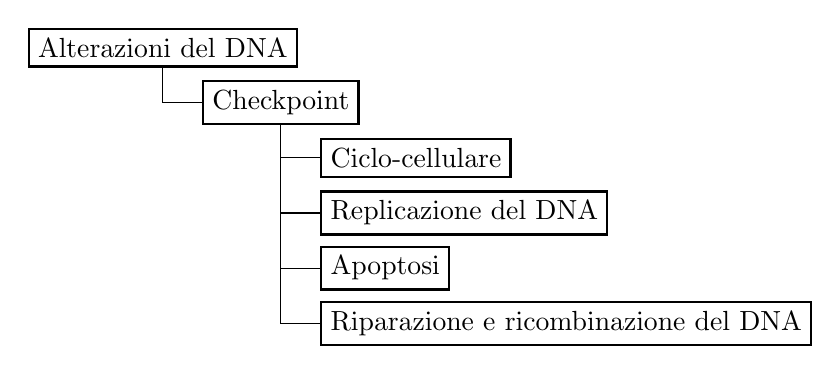
\begin{tikzpicture}[%
    grow via three points={one child at (0.5,-0.7) and
    two children at (0.5,-0.7) and (0.5,-1.4)},
    edge from parent path={(\tikzparentnode.south) |- (\tikzchildnode.west)}]
    \node {Alterazioni del DNA}
        child { node {Checkpoint}
            child { node {Ciclo-cellulare}}
            child { node {Replicazione del DNA}}
            child { node {Apoptosi}}
            child { node {Riparazione e ricombinazione del DNA}}
        };
\end{tikzpicture}
\end{large}
\end{center}
Ad eccezione di altre molecole il DNA può essere riparato.\\
Il danno può essere riparato:
\begin{itemize}
    \item Direttamente
    \item Per escissione della zona del danno o di zone contigue
    \item Per ricombinazione
\end{itemize}
\subsection{I principali meccanismi di riparazione del DNA alterato}
I principali meccanismi di riparazione del DNA alterato sviluppati dalle cellule possono essere divisi in:
\begin{itemize}
    \item \textbf{NER[Nucleotide Excision Repair - riparo per escissione di nucleotidi]}\\
    Il meccanismo NER è utilizzato per riparare la maggior parte delle lesioni del DNA. è un sistema molto versatile, costituito da vari enzimi che sono in grado di riconoscere il danno e successivamente di eliminare la porzione dell'elica contenente il danno.\\
    La porzione di DNA eliminata viene in seguito risintetizzata utilizzando l'altro filamento di DNA come stampo.
    \item \textbf{BER [base Excision repair - riparo per rimozione di basi]}\\
    Il riconoscimento della lesione (che in questo caso si tratta di una base alterata) avviene ad opera di N-glicosidasi che è in grado di idrolizzare il legame glicosidico e di staccare la base alterata. La base così rimossa può talvolta essere reinserita ad opera di una insertasi.
    \item \textbf{Mismatch Repair}\\
    Questo meccanismo è in grado di riparare alterazioni che si verificano nel DNA durante la replicazione Il tipo di danno in questo caso riguarda un incorretto appaiamento delle basi (errore replicativo).
    \item \textbf{Riparo post replicazione [o riparo per ricombinazione]}\\
    \item Con il termine di riparo post-replicatico si intende un sistema in grado di aggire su un DNA in cui il filamento figlio abbia replicato nonostante sul filamento parentale siano ancora present delle lesioni.\\
    La riparazione avviene attraverso l'induzione di un meccanismo di ricombinazione che porta allo scambio di filamenti singoli.
\end{itemize}
\subsubsection{Riparazione per escissione di Nucleotidi (NER)}
È un sistema che interveniene per riparare il DNA da lesioni che causano distorsione della doppia elica (es. da agenti
chimico-fisici).\\
Sistema utilizzato per riparare danni da UV (tra cui dimeri di pirimidina).\\
Meccanismo del NER nei mammiferi. In tutti gli eucarioti il NER è diviso in due sotto-pathway chiamati Global Genome NER (GG- NER) e Transcription-Coupled Repair (TCR-NER).
I due sotto-pathway si distinguono nelle fasi iniziali del processo per poi convergere in un unico meccanismo comune.\\
Nel GG-NER (fase A, a sinistra), il complesso proteico XPC-hHR23B individua regioni in cui il corretto appaiamento tra i
due filamenti del DNA è alterato a causa di una distorsione della doppia elica.\\
Nel TCR-NER (fase A, a destra) diversi tipi di lesione nelle regioni trascritte determinano un blocco delle RNA polimerasi
(particolarmente studiata è l'RNA polimerasi II) che devono essere rimosse dal DNA per permettere la riparazione dei danni. Questo evento richiede due proteine specifiche del TCR-NER, chiamate CSA e CSB.\\
\paragraph{}I passaggi successivi del GG-NER e del TCR-NER sono
essenzialmente identici.
Il complesso multiproteico TFIIH, che contiene due polipeptidi chiamati XPB e XPD con attività DNA elicasica (fase B), apre il DNA per un tratto di circa 30 nt (nucleotidi) attorno alla lesione.
La proteina XPA conferma la presenza della lesione legandosi a
essa (fase C), altrimenti tutta la reazione termina a questo stadio. La regione del DNA aperta dall'azione dell'elicasi è
stabilizzata dal legame con la proteina RPA che ha un'elevata affinità di legame per il DNA a singolo filamento.
XPG e ERCC1/XPF sono due endonucleasi NER-specifiche che tagliano, rispettivamente, in 3' (destra) e in 5' (sinistra) il filamento di DNA contenente la lesione, generando un frammento di circa 30 nt che verrà poi eliminato (fase D).
\paragraph{}È stato così generato un buco di 30 nt con un'estremità 3'OH nel
filamento danneggiato che può ora essere riparato dai normali
enzimi che replicano il DNA copiando il filamento complementare
che non è stato danneggiato (fase E). Studi in vivo, in cui si riesce a valutare la cinetica di legame dei diversi componenti del NER al
DNA danneggiato, dimostrano che i singoli fattori proteici si assemblano nell'ordine indicato nella figura: la riparazione della
lesione richiede, nel suo insieme, alcuni minuti, dopo di che l'intera "macchina" riparativa viene disassemblata.
\subsubsection{Riparazione per escissione delle basi (BER) negli eucarioti}
Questo meccanismo ripara danni endogeni causati da stress ossidativo o da danni esogeni causati sulle basi azotate da agenti mutageni.\\
Esistono due vie del BER, chiamate "short-patch" o "long-patch": nel primo caso viene
sostituito soltanto il nucleotide con la base alterata (X), nel secondo la regione di DNA riparata è di una decina di nucleotidi.\\
Il primo step è il riconoscimento del danno da riparare.\\
Danni causati da specie reattive dell'ossigeno (ROS) quali metilazioni o deaminazioni. DNA glicosilasi specifiche riconoscono il tipo di lesione, rompono il legame glicosidico tra zucchero e base azotata danneggiata.\\
Le DNA glicosilasi una volta identificata la base alterata comprimono la doppia elica e la base alterata viene quindi inglobata all'interno della glicosilasi. La glicosilasi taglia quindi il legame glicosidico e si crea un sito
senza base (sito AP). Il sito AP può anche formarsi per idrolisi spontanea. APE1, una endonucleasi, riconosce il sito senza base e taglia il legame fosfodiesterico.\\
Meccanismo BER procede quindi attraverso 2 vie: short-patch BER (revalente nei mammiferi) e long-patch BER.
\paragraph{Short-patch BER}DNA polimerasi beta rimuove il deossiribosio e poi riempie il buco
formatosi. La DNA ligasi 3 salda il legame fosfodiesterico con l'aiuto della proteina XRCC1.
\paragraph{Long-patch BER}DNA polimerasi $\delta $ o $\varepsilon $ insieme alla proteina
PCNA allungano 3'OH (di circa 2-10 nucleotidi) mediante la reazione di strand displacement. Il
filamento di DNA è poi tagliato dalla nucleasi FEN1 che riconosce la struttura. Interveniene quindi la DNA lgasi 1 che salda la discontinuità del filamento.
\subsubsection{Mismatch Repair (MMR) negli eucarioti}
L'apparato enzimatico che agisce durante la replicazione del DNA (tre polimerasi principali, DNA polimerasi $\alpha, \delta, \varepsilon$) può
compiere alcuni errori. Per esempio, sul filamento neosintetizzato può venire inserita
una base sbagliata, generando l'appaiamento non complementare A-C, o si possono formare delle piccole bolle (indicate in rosso) dovute allo scivolamento
dell'apparato replicativo in corrispondenza di sequenze nucleotidiche ripetute.\\
Tali strutture anomale sono, dapprima, riconosciute dai complessi chiamati MutS$\alpha$ e MutS$\beta$ che reclutano, successivamente, i complessi MutL$\alpha$ e MutL$\beta$.
Il filamento di DNA neosintetizzato contenente gli errori replicativi viene riconosciuto e processato da una esonucleasi (Exo1) che degrada il filamento di DNA in direzione 5' $\sim $ 3'.
Successivamente, attraverso interazioni con tutto l'apparato di replicazione, viene ri-sintetizzato il filamento di DNA corretto.
\subsection{Meccanismi di tolleranza al danno}Nel caso in cui un danno al DNA non venga riparato e viene
generato un filamento alterato si verifica, per la maggior parte delle lesioni, un ostacolo ad una successiva replicazione.
Un blocco della replicazione sarebbe però letale per la cellula. Ecco quindi che intervengono dei meccanismi di tolleranza al danno che permettono la replicazione del DNA danneggiato.\\
Tali meccanismi vengono indicati come «Post-Replication Repair (PRR).
\begin{center}
    \includegraphics[width=1\textwidth]{danno.png}
\end{center}
\begin{itemize}
    \item{(A)}attraverso un cambiamento dello stampo, definito "template switch": il filamento di neosintesi che copia
    il filamento di DNA stampo danneggiato si sposta a copiare il filamento neosintetizzato complementare
    allo stampo privo della lesione;
    \item{(B)}attraverso la sintesi di DNA translesione (TLS), che prevede l'utilizzo di diverse TLS polimerasi che
    possono introdurre nucleotidi corretti ("error free") o sbagliati ("error prone") di fronte alla lesione.
    \item{(C)}Alternativamente, l'apparato replicativo, utilizzando proteine quale il complesso DNA polimerasi $\alpha$-
    primasi, può saltare la lesione, facendo ripartire la replicazione del DNA a valle del danno (C). Questo
    meccanismo lascia un tratto di DNA non replicato che può essere riempito, ancora una volta, tramite
    "template switch" (D) o sintesi di DNA TLS (E).
\end{itemize}
\subsection{Riparazione di rotture su doppio filamento (Double Strand Break DSB)}
\textit{Sono le alterazioni più pericolose}\\
La riparazione di DSB avviene tramite meccanismi diricombinazione alquanto complessi.
I DSB sono riparati attraverso due vie principali: la prima via è chiamata "Homologous Recombination" o HR e richiede l'azione coordinata di numerose proteine, la seconda via è chiamata NHEJ (Non-Homologous End Joining).
\subsubsection{Homologous Recombination" o HR}
\begin{center}
    \includegraphics[width=0.70\textwidth]{HR.png}
\end{center}
Nel meccanismo di HR, il complesso eterotrimerico Mre11/Rad50/Nbs1 (chiamato MRN) con l'ausilio di altre proteine
(fra cui Rad51 e Rad52) modifica il DSB originario causando la degradazione in direzione 5' 3' delle due estremità 5' di ciascun DSB.
Si generano, così, delle regioni di DNA a singolo filamento che sono stabilizzate dal legame della proteina RPA (fase b).
Successivamente la proteina Rad51, con l'ausilio di Rad52 e altre proteine ricombinative, scalza RPA e forma un filamento
nucleoproteico in cui il DNA a singolo filamento è ricoperto da Rad51 (fase c).\\
L'estremità 3'OH del filamento coperto da Rad51, con l'aiuto di altre proteine ricombinative, procede ora alla ricerca di sequenze
omologhe di DNA presenti sul cromosoma omologo (o sul cromatide fratello) non danneggiato, formando quella che viene chiamata una giunzione di Holliday.
La perdita di Rad51 all'estremità 3'OH innesca la neosintesi di DNA (fase e); la risoluzione degli intermedi di ricombinazione da parte di proteine
specifiche, qui genericamente indicate come risolvasi, e l'azione della DNA ligasi generano due molecole riparate (fase f). Mediante il meccanismo chiamato SDSA (Synthesis Dependent Strand Annealing) il DNA
neosintetizzato si stacca dopo un po' dallo stampo che sta copiando e ritorna sulla molecola di DNA originariamente danneggiata.
\subsubsection{NHEJ (Non-Homologous End Joining)}Nel processo di NHEJ le estremità del DSB sono riconosciute da
un complesso noto come Ku70/Ku80 che interagisce con una proteina chinasi, chiamata DNA-PK .
Può accadere che le estremità del DSB siano processate in modo limitato localmente con il possibile intervento del complesso Mre11/Rad50/Nbs1 (MRN) (fase b).
Infine, sono reclutate le proteine XRCC4 e la DNA ligasi 4 la cui azione porta alla saldatura diretta delle estremità rotte (fase c).
\begin{center}
    \includegraphics[width=0.70\textwidth]{DSBR.png}
\end{center}
\section{Riparazione diretta}
\subsection{Riparazione del DNA mediante fotoriattivazione} Sistema di riparo che elimina direttamente il danno (dimeri di timina da luce UV). L'enzima \textbf{fotoliasi assorbe da sole l'energia necessaria per rompere i legami che uniscono le due pirimidine.}\\
Tra i meccanismi di riparazione direttamente sui nucleotidi c'è MGMT (O-6- metillguanina-DNA metilltransferasi), che rimuove specificamente alterazioni chimiche a carico della guanina
\section{La ricombinazione genetica}
\paragraph{Meccanismo di cromotripsi}Evento cromosomico catastrofico in cui si verificano più rotture del doppio filamento, limitato ad una semplice segmento
cromosomico o ad alcune regioni cromosomiche. La cromotripsi consiste nella formazione di frammenti cromosomici che vengono riassemblati insieme in maniera caotica.\\
Da studi su cellule tumorali e condotti su pazienti con disordini congeniti, è stato possibile identificare alcuni criteri di riconoscimento della cromotripsi:
\begin{itemize}
    \item Il fenomeno avviene in un unico catastrofico evento (generando decine o centinaia di
    riarrangiamenti localizzati su uno o pochi cromosomi) e si osserva , la tendenza dei punti di
    rottura e di giunzione a raggrupparsi in piccoli segmenti cromosomici (fino a 10 punti di rottura
    nell'arco di 50 Kb);
    \item La frammentazione dei cromosomi interessati causa una diffusa perdita di sequenze nucleotidiche;
    \item I frammenti cromosomici derivano dalla frantumazione di un solo cromosoma parentale e
    generalmente vengono riassemblati senza alcun orientamento preferenziale o ordine;
    \item Nei punti di rottura non si riscontra omologia (al limite alcune micro-omologie di pochi nucleotidi).
\end{itemize}
Non è ancora noto il meccanismo che innesca la cromotripsi, e sono stati ipotizzati diversi meccanismi:
La frammentazione del cromosoma può avvenire come risultato di una mis-segregazione durante la mitosi:
Esposizione a stimoli esogeni, radicali liberi o radiazioni ionizzanti durante la mitosi,
Stress replicativo (coinvolto nel rendere più probabile un fenomeno di riarrangiamento genomico complesso)
Una TP53 mutata potrebbe avere un ruolo nel favorire la sopravvivenza della cellula all'evento catastrofico della cromotripsi.\\
\subsection*{La ricombinazione genetica}
\begin{center}
    \includegraphics[width=0.70\textwidth]{ricombinazione.png}
\end{center}
Funzione principale della ricombinazione è creare nuove combinazioni di geni.\\
La variabilità genetica consente alle specie di evolversi con il cambiare delle condizioni ambientali.
\subsection{Tipi di ricombinazione}
\begin{itemize}
    \item \textbf{Ricombinazione tra sequenze omologhe:}\\
    (generalized o Homologus recombination) avviene prevalentemente nella meiosi. Avviene allo stadio di "four strand".
    \item \textbf{Ricombinazione tra paia di sequenze specifiche:}\\
    site specific ricombination. Es. nell'integrazione dei fagi. Gli enzimi sono specifici per la sequenza.
    \item \textbf{Trasposizione:}\\
    sequenze vengono inserite senza bisogno di omologia di sequenza.
\end{itemize}
\subsubsection{Ricombinazione omologa}
La ricombinazione permette di separare i vari geni nel genoma e di separare le mutazioni favorevoli da quelle sfavorevoli.\\
Le ricombinazioni avvengono tra sequenze che corrispondono perfettamente, così da non perdere nessuna base dal cromosoma ricombinante.\\
La frequenza non è costante ma varia con effetti globali e locali.
\begin{enumerate}
    \item Allineamento di due molecole di DNA omologhe.
    \item Introduzione di rotture del DNA
    \item Formazione di una corta regione di appaiamento: invasione del filamento e formazione dell Holliday junction.
    \item Movimento della Holliday junction - branch migration.
    \item Taglio della giunzione: risoluzione.
\end{enumerate}
\subsubsection{Modello di Holliday}
I DNA si appiano, si ha un taglio ai siti corrispondenti, le terminazione libere si complementano all'altro duplex: Joint molecule e Joint recombination.\\
Il sito di ricombinazione: DNA ibrido o heteroduplex. Esso migra e deve essere catalizzato da enzimi.\\
La joint molecule deve essere risolta da due tagli. Se esso è sullo stesso strand si ottiene una zona heteroduplex: patch recombinant. Se è sull'altro strand, tutti gli strand sono stati tagliati e si ha ricombinazione: splice recombinant.
\begin{center}
    \includegraphics[width=0.70\textwidth]{ricombinazione2.png}
\end{center}
Modello di Holliday applicato a una rottura a doppio filamento (DSB) sul DNA. Nel modello di ricombinazione che
coinvolge un DSB l'evento scatenante è la produzione del DSB stesso (I). Le estremità 5' del DSB sono processate così
da generare delle estremità 3'OH sporgenti a singolo filamento (II). Una (III) o entrambe le estremità 3'OH possono
invadere la molecola di DNA omologa dando origine a neosintesi riparativa del DNA (indicata in rosso) attraverso
l'estensione delle estremità 3'OH e copiatura del filamento complementare intatto (IV).\\
Alla fine del processo di ricombinazione di un DSB può generarsi un intermedio con due giunzioni di Holliday (V), che
indichiamo come x e y. Tale intermedio sarà risolto da reazioni di taglio e ricucitura come descritto e la struttura finale delle
molecole ricombinanti che si formeranno è, di nuovo, influenzata dalle modalità con cui le giunzioni vengono tagliate. Per ogni
giunzione x e y ci sono due possibilità di taglio, indicate come sito di taglio 1 o 2. Se entrambe le giunzioni vengono tagliate allo
stesso sito di taglio (1 o 2) si avrà la formazione di prodotti "patch" (o del non-crossing over), come mostrato nell'esempio in
VIa, dove entrambe le giunzioni sono state tagliate al sito 2. Infatti, gli alleli A/B e a/b fiancheggianti le giunzioni si ritrovano
nella stessa combinazione presente nelle molecole prima della ricombinazione (lo stesso accade se entrambe le giunzioni
vengono tagliate al sito 1: infatti, anche se il taglio alla giunzione x genererebbe un prodotto di crossing over, questo effetto
viene, di fatto, annullato dal taglio al sito y: crossing over + crossing over = non-crossing over). Viceversa, se le due giunzioni di
Holliday sono tagliate a siti diversi (VIb) si ha la formazione dei prodotti di crossing over, con il riassortimento degli alleli
fiancheggianti le giunzioni.
\subsubsection{Risoluzione della riparazione del DSB}
Se i tagli avvengono simmetricamente si risolve in un patch.\\
Se asimmetrici nella ricombinazione.
\paragraph{Gameti ricombinanti}
Gameti con combinazioni alleliche diverse da quelle dei genitori.\\
Il crossing-over è il meccanismo alla base della produzione di gameti ricombinanti! Per ogni singolo crossing-over si formerano metà gameti ricombinanti e metà non ricombinanti.
\subsubsection{Ricombinazione sito specifica}Si riferisce a specifiche sequenze del DNA anche molto corte (20-200 nucleotidi)
Integrazione del genoma del batteriofago $\lambda$
\paragraph{Batteriofago $\lambda$} è un virus che infetta E.Coli.
\begin{itemize}
    \item Il suo genoma è una molecola di DNA lineare a dobbio filamento di 48.5 kB.
    \item Le estremità presentano un'estensione a singolo filamento di 12 bp complementari (sito cos) che ne consentono la circolarizzazione una volta entrato nell'ospite.
    \item Le sequenze responsabili della Ricombinazione (att)
    \item Geni funzionalmente correlati sono raggruppati in regioni distinte cI (regolatore negativo), N e Q (regolatori positivi).
    \subitem{-} Regolanti il passaggio dal ciclo lisogenico al ciclo litico N, cI (cII e cIII) e cro
    \subitem{-} Sintesi del DNA (O,P)
    \item e i geni che codificano per proteine della Testa (Head) e Coda (Tail):
    \subitem{-} Funzioni tardive (Q)
    \subitem{-} Lisi dell'ospite (S,R)
\end{itemize}
La funzione biologica dell'integrazione determina uno stato lisogenico per cui il DNA del fago si replica passivamente insieme a quello batterico.\\
Quando il DNA del fago viene escisso dal genoma batterico si ha una replicazione indipendente del fago: vengono prodotte molte copie di DNA e provocata la lisi batterica.
\paragraph{Replicazione del fago $\lambda$}Quando il fago i infetta il batterio le estremità coesive si appaiano formando una struttura circolare (il sito cos è sensibile alla temperatura, che le
denatura) e i nicks sono riparati dalla ligasi batterica.
L'integrazione del genoma fagico all'interno di quello batterico avviene presso una speciale regione. La sequenza precisa sul genoma di E. coli è
chiamata attB (dall'inglese Bacterial attachment, sito di attacco batterico) ed è composta essenzialmente di tre segmenti, detti B-O-B'. La
sequenza omologa sul genoma del fago è attP (dall'inglese Phagic attachment, sito di attacco fagico) ed è composta delle regioni P-O-P'.
Il sito di attacco sul DNA del fago 1 (attP) possiede solo 15 bp completamente omologhe al sito batterico (attB). La reazione operata dalla
integrasi (INT, ricombinasi di X) genera due nuovi siti di attacco, che fiancheggiano il DNA fagico inegrato (attR e att.).
La proteina XIS (codificata dal fago) insieme alle proteine batteriche FIS e IHF procedono invece alla rimozione del DNA del fago.\\
\begin{center}
    \includegraphics[width=0.70\textwidth]{batteriofago.png}
\end{center}
II DNA circolare del fago viene duplicato in questa fase come plasmidi (replicazione theta). Poi passa ad un modello di rolling circle generando una molecola di DNA lineare contenente un gran
numero di copie genomiche continue. In questa modalità il fago si trova nel ciclo litico.


\begin{titlepage}
    \begin{center}
        \vspace*{1cm}
        \LARGE
        Trasposoni
            
        \vspace{1.5cm}
        
        \Large
        \textbf{Lezione 10 - Marzo 2021}

        \vspace{0.8cm}

    \end{center}
\end{titlepage}
\setcounter{page}{39}
\section{Trasposoni}
Gli elementi trasponibili (TEs, Transposable Elements) sono sequenze di DNA in grado di "muoversi" da
un sito all'altro del genoma,
Creando o revertendo mutazioni sono in grado di alterare il genotipo cellulare.
Tali elementi furono scoperti per la prima volta da Barbara McClintock in Zea mays negli anni '40
da allora i TEs sono stati identificati in una notevole varietà di organismi eucariotici e si è scoperto che
costituiscono circa il 45$\%$ del genoma dei mammiferi e fino al 90$\%$ del genoma di alcune specie di
piante .
I TEs essendo mobili, sono in grado sia di cambiare il loro intorno genomico sia quello del locus entro il
quale si integrano.
Inoltre, dal momento che hanno la capacità di replicarsi durante il processo di trasposizione, essi sono
inevitabilmente presenti in un notevole numero di copie nel genoma e si possono considerare sia parte
del genoma che entità indipendenti che vivono al suo interno.
\begin{itemize}
    \item[A. ] Trasposoni a DNA
    \item[B. ] Retrotrasposoni:
        \subitem retrotrasposono LTR\\(es. retrovirus caratterizzati da lunghe sequenze ripetute)
        \subitem retrotrasposoni non LTR\\
        In entrambi i casi contengono sequenze utili per la reazione di ricombinazione.\\
        Contengono inoltre l'enzima utile alla trasposizione ovvero l'integrasi o trasposasi.\\
        I retrotrasposoni codificano anche per la loro trascrittasi inversa (polimerasi in grado di copiare uno stampo di RNA in DNA).
\end{itemize}

\subsection{Trasposoni a RNA}
Trasposoni a DNA costituiscono circa il 3$\%$ del genoma umano.
Generalmente contengono contengono sequenze terminali ripetute e invertite, che
circondano una ORF (Open Reading Frame), che codifica per l'enzima trasposasi.
L'mRNA risultante dalla trascrizione del trasposone viene tradotto, portando alla sintesi
dell'enzima trasposasi; la trasposasi una volta trasferita nel nucleo, lega all'interno o nelle vicinanze del trasposone
le sequenze terminali ripetute e invertite, "taglia" il trasposone e lo "incolla" in un'altra
posizione nel genoma.
Praticamente tutti i trasposoni a DNA del genoma umano sono mutati, incapaci quindi di trasporsi da una regione ad un'altra del genoma.
\begin{center}
    \includegraphics[width=1.10\textwidth]{batteri.png}
\end{center}

\section{Retrovirus}
\subsection{Retrotrasposoni LTR}
Sono retrovirus caratterizzati da lunghe sequenze ripetute.\\
Si tratta di aggregati molecolari privi di organelli che ne permettano la replicazione.\\
Dunque se i retrovirus non penetrano in una cellula non riescono a duplicarsi.\\
Esternamente presentano un involucro fosflipidico detto \textbf{capside o enveloper}. Allìnterno è contenuto il genoma costituito da due molecole di Rna.
Il genoma virale contiene almeno tre geni fondamentali.
\begin{itemize}
    \item GAG(group specific antigen)\\
    Codifica per le proteine strutturali
    \item POL(polymerase)\\
    Codifica per l'enzima Trascrittasi Inversa
    \item ENV(enveloper)
    Codifica per le proteine di membrana
\end{itemize}
\subsection{Ciclo vitale di un retrovirus}
Ciascuna particella
virale contiene due molecole di RNA di circa
8000-10 000 nucleotidi (in rosso). Tramite
l'attività della trascrittasi inversa si genera una
molecola ibrida RNA:DNA e, successivamente,
una molecola di DNA a doppio filamento (qui
indicata in verde per distinguerla dal DNA
genomico). Questo DNA copia o provirus
viene introdotto nel genoma della cellula
infettata mediante l'azione di un enzima,
anch'esso codificato dal virus, e chiamato
integrasi. Questa integrazione è richiesta per
la sintesi, da parte dell'RNA polimerasi della
cellula, di nuove molecole di RNA virali.
\paragraph{Il provirus formato dal funzionamento della trascrittasi inversa è più lungo del genoma}
Le estremità caratteristiche del genoma contengono una sequenza R e la sequenza unica U5 ad un'estremità, e
U3 e R all'estremità opposta.
A seguito dell'attività della trascrittasi inversa due sequenze identiche, U3, R e U5, vengono ad essere formate e
localizzate all'estremità 5' e all'estremità 3'.
Queste sequenze sono note come Long Terminal Repeats (LTR), e svolgono un ruolo determinante nel
controllare il processo di trascrizione che porterà alla sintesi, partendo dal provirus, degli RNA messaggeri virali.
Quindi il provirus è più lungo, due sequenze LTR identiche sono presenti all'estremità 3' e all'estremità 5'.
La trascrittasi inversa, come le RNA polimerasi RNA dipendente è un enzima estremamente inaccurato ed è
stato calcolato che, una volta che copia il genoma ad RNA, può introdurre in questo genoma ben da 1 a 10
errori, quindi un tasso mutazionale elevato, che comporta un enorme variabilità.
\paragraph{}
Il DNA a doppio filamento va nel nucleo e, grazie all'intervento
dell'integrasi, (attività enzimatica presente nel core virale) viene ad
essere integrato nel cromosoma della cellula. A questo punto è
chiamato provirus.
L'RNA polimerasi II della cellula è in grado di trascrivere i
geni del provirus arrivando alla sintesi dei messaggeri
cellulari.
\begin{center}
    \includegraphics[width=1\textwidth]{retrovirus.png}
\end{center}
\subsection{I retroelementi}
I retroelementi contenenti LTR compongono circa l'8$\%$ del nostro genoma.
I retrovirus endogeni HERV fanno parte dei retrotrasposoni LTR e somigliano ai retrovirus
nella struttura e nella mobilità; molti HERV contengono un gene ENV non funzionante, che
perciò li relega ad un'esistenza intracellulare.
Le loro lunghe ripetizioni terminali, sequenze regolative importanti per la mobilità, fiancheggiano
una regione centrale codificante per tutte le proteine generalmente prodotte dai genomi
retrovirali, fatta eccezione per quelle codificate da ENV
Praticamente tutti gli HERV sono stati resi inattivi da eventi mutazionali e quindi non sono
capaci di retrotrasposizione autonoma;
soltanto la famiglia HERV-K, presente nell'uomo e nelle scimmie antropomorfe e quindi
evolutivamente recente, conserva delle copie intere non mutate del genoma virale e rimane
potenzialmente infettiva.\\
LTR contengono sequenze che regolano la trascrizione, Non-LTR la trascrizione è regolata da promotori interni.
I retrotrasposoni non-LTR comprendono le classi degli
elementi LINEs (Long Interspersed Elements) e SINEs
(Short Interspersed Elements).
\section{Retrotrasposoni non LTR (senza terminali ripetuti)}
Gli elementi NON-LTR sono i LINE e SINE.\\
Gli elementi LINE (i più abbondanti), hanno un promotore per la polimerasi II e codificano per due ORF (una con capacità di
legame all'RNA e l'altra con attività di endonucleasi e reverse trascrittasi). Sono AUTONOMI (L1,L2,L3). Sono presenti
molte copie tronche soprattutto di L1.\\
Gli elementi SINE hanno un promotore per la polimerasi III, e non codificano proteine ma dipendono dall'attività dei LINE,
NON AUTONOMI.\\
Un classico esempio di SINE sono le sequenze Alu (circa 300 bp). Ne sono presenti fino a 500000 copie nel genoma umano
(11$\%$). Sono ripetizioni specifiche dei Primati, pur se altri Mammiferi hanno sequenze simili.
Un altro tipo di retrotrasposone NON-AUTONOMO, che usa l'apparato di L1 per trasporsi nel genoma è "SVA": un elemento
ripetuto composito (SINE+VNTR+ALU).Possono essere individuate dal fatto che sono capaci di legare l'enzima Alu I.\\
Ricerche recenti hanno suggerito che le LINE e le SINE possano aver avuto sia un ruolo importante
nell'evoluzione dei genomi, sia significativi effetti a livello strutturale e trascrizionale.
Le sequenze LINE-1 sono gli unici retrotrasposoni umani autonomamente attivi conosciuti,
e costituiscono approssimativamente il 17$\%$ del nostro genoma.\\
I retroelementi LINE-1 capaci di retrotrasposizione ed hanno un promotore interno per la
RNA polimerasi II che dirige la trascrizione del retroelemento a partire dall'estremità. Sono
in grado di codificare anche per la proteina ORF1p e per per la proteina ORF2p con
attività di endonucleasi e di trascrittasi inversa, necessarie per la retrasposizione di Line-1.
\subsection{Trasposoni autonomi e non}
\begin{itemize}
    \item Trasposoni autonomi:\\
    in grado di eseguire in modo autonomo la propria trasposizione: hanno
    sequenze di DNA in cis per la reazione di ricombinazione
    Porzioni codificanti per la trasposasi e trascrittasi inversa
    \item Trasposoni non autonomi:\\
    possono trasporsi solo in cellule dotate di trasposoni autonomi
    Hanno solo le sequenze di DNA in cis per la ricombinazione.\\
    questi retroelementi non autonomi
    consistono principalmente nelle sequenze
    Alu (SINE, Short INterspersed Element),
    che compongono circa il 10-11$\%$ del genoma umano.
\end{itemize}
Dal momento che gli elementi trasponibili sono in grado di replicarsi più
velocemente del genoma, essi possono essere visti come parassiti che conferiscono
svantaggi al genoma che abitano
Per questo motivo sono stati a lungo considerati DNA "spazzatura", ovvero una
porzione del genoma che, benché fosse consistente, non mostrasse alcuna
funzione,
Questa visione semplicistica è stata notevolmente rivista, infatti si è osservato che i
TEs e i genomi hanno co-abitato per molto tempo, e quindi che hanno interagito
in molti modi differenti, e inoltre è stato riportato che tali elementi potrebbero
avere importanti ruoli sia regolativi che strutturali, nonostante siano stati a lungo
considerati privi di alcuna funzione apparente.
Per tali motivi gli elementi trasponibili sono ormai considerati , come elementi
interni al genoma stesso che ne hanno guidato l'evoluzione.

\paragraph{}I retrotrasposoni non-LTR comprendono una estesa porzione del genoma
specialmente in piante e mammiferi, e l'effetto del loro aumento è stato
tollerato durante l'evoluzione.
Sono ormai riportati molti esempi di quanto gli elementi ripetuti siano utili
strumenti per studiare l'evoluzione del genoma e la funzione dei geni.
Un'analisi comparativa, per esempio, ha messo in luce che molte sequenze
umane di elementi trasponibili sono identiche a quelle degli altri vertebrati e,
inoltre, che l'inserzione di TEs può regolare l'espressione genica, aumentare la
ricombinazione e il crossover ineguale.
Lo studio di questi tratti di DNA è importante per la genetica di popolazione
dell'uomo e per l'evoluzione dei primati, in particolare per l'evoluzione
umana.
Le sequenze Alu formano nei primati un registro fossile relativamente semplice da
decifrare in quanto gli eventi di inserzione delle sequenze Alu sono fedelmente
trasmessi di generazione in generazione e sono facilmente identificabili. Lo studio
di queste sequenze può rivelare quindi relazioni di discendenza in quanto due
individui condivideranno una particolare inserzione se hanno un antenato
comune. La maggior parte delle sequenze Alu nel genoma umano possono essere
riscontrate anche nelle corrispondenti posizioni dei genomi di altri primati, tuttavia
circa 7.000 inserzioni Alu sono tipiche degli esseri umani L'inserzione di sequenze
Alu è implicata in diverse malattie ereditarie umane e in varie forme di cancro.
\paragraph{La Neurofibromatosi di tipo 1 (NF1)} o malattia di von Recklinghausen fa parte di un gruppo
di malattie genetiche multisistemiche e progressive dette Facomatosi o anche sindromi
"neurocutanee": tumori a carico della pelle e dei nervi. La NF1 ha un'incidenza di 1 su
2500-3000 nati ed una prevalenza di circa 1 su 4000-5000 individui nella popolazione
generale. Si trasmette con modalita' autosomica dominante, il 50$\%$ dei casi sono sporadici. Il
gene NF1 è stato localizzato in sede pericentrometrica del braccio lungo del cromosoma 17.
E' un gene oncosoppressore di oltre 335 kb di DNA genomico, con almeno 60 esoni, che
codifica per una proteina di 2818 aa chiamata neurofibromina che si localizza nei
microtubuli citoplasmatici e che svolge una regolazione negativa della crescita cellulare con
attività di controllo di attivazione sul ras pathway. Da qui la funzione di soppressore di
tumore svolto dalla neurofibromina. Nel 1991 è stato scoperto, in un uomo di 31 anni
affetto da neurofibromatosi, che il danno genetico era stato causato da una trasposizione
della sequenza Alu in uno degl introni di NF1: errore nello splicing con errata rimozione di
un esone. I genitori erano entrambi privi della sequenza Alu in quell'introne.
\section{Trasosoni in E.Coli}
I trasposoni si trovano sia nei procarioti sia negli eucarioti
In E.coli (e in generale nei batteri) tre tipi di elementi
trasponibili:
\begin{itemize}
    \item Sequenze di inserzioni (IS)
    \item Trasposoni composti
    \item Fagi trasponibili
\end{itemize}
\subsection{Elementi IS}
\begin{center}
    \includegraphics[width=1\textwidth]{IR.png}
\end{center}
\begin{itemize}
    \item Sono il tipo più semplice di trasposoni. Si trovano, a volte in
    numero molto elevato, sia nel cromosoma batterico sia nelle
    molecole epigenetiche come i plasmidi.
    \item Codificano solamente il gene per la mobilizzazione. 
    \item Hanno dimensioni che vanno da 768 bp a 5 kb.
    \item IS1 è stata la prima IS ad essere stata identificata nell'operone
    galattosio di E. coli. Essa presenta dimensioni di 768 bp ed è
    presente in un numero di copie che va da 4 a 19 nel cromosoma di
    E. coli.
    \item Tutte le IS presentano alle loro estremità delle sequenze ripetute
    ed invertite.
\end{itemize}
\subsection{Trasposoni composti}
Essi contengono e trasportano geni (come ad esempio
quelli per la resistenza agli antibiotici) fiancheggiati ad
entrambe le estremità da elementi IS.\\
Tn10 è un esempio di trasposone composto. Le sue
dimensioni sono di 9.3 kb di cui 6.5 kb di DNA centrale
(contenente il gene per la resistenza alla tetraciclina)ed
un totale di 1.4 kb di elementi IS.\\
Almeno una IS fornisce la trasposasi mentre entrambe
forniscono le sequenze ripetute ed invertite.
\begin{center}
    \includegraphics[width=1\textwidth]{Trasposizione.png}
\end{center}
La trasposizione di un elemento IS o di un trasposone
composto genera la duplicazione di una sequenza di DNA. In
seguito al meccanismo d'azione della trasposasi, si genera la
duplicazione di una breve sequenza del DNA bersaglio a livello
del sito d'integrazione del trasposone.
\subsection{Mu - il fago trasposone che si integra sempre}
Il DNA del fago Mu si integra in qualunque sito del genoma dell'ospite come i trasposoni. Allo stato lisogeno determina quindi l'inattivazione nel gene in cui si è inserito.
\begin{center}
    \includegraphics[width=0.70\textwidth]{Mu.png}
\end{center}
L'inversione del segmento G determina un cambiamento
nell'espressione dei geni che codificano le proteine della fibra della
coda del fago. Queste determinano la specificità d'ospite.\\
L'inversione è mediata dalla proteina codificata dal gene gin.\\
All'interno del Mu si può riconoscere un modulo traspositivo caratterizzato dal gene A che codifica per la trasposasi, il gene B che codifica per una DNA binding protein (ATP-dipendente)
richiesta per un'efficiente trasposizione e le due sequenze Mu-att che sono i bersagli della trasposasi.11
Il sito Mu-attR è separato da circa 30Kb dal resto del modulo trasposone.
\subsubsection{I repressori del ciclo litico di Mu}
All'interno del modulo traspositivo ci sono due regolatori C e Ner che sono essenziali per la trasposizione.\\
C codifica per il repressore richiesto per il mantenimento dello stato lisogenico.
C reprime i geni per la trasposasi e compete con la trasposasi per i siti Mu-att.\\
Ner controlla negativamente la trascrizione dei geni necessari per lo sviluppo del fago.
\subsubsection{Integrazione del fago Mu nel cromosoma}
Sia per il ciclo litico che per il ciclo lisogenico il fago Mu si integra nel cromosoma.\\
\begin{itemize}
    \item L'integrazione è mediata dalla trasposasi sintetizzata dal fago.
    \item Avviene un taglio sfalsato nel Dna dell'ospite.
    \item In seguito all'integrazione del fago la polimerasi dell'ospite replica i tratti a DNA SS generando così duplicazioni direttamente ripetute all'estremità del fago (5bp)\\
\end{itemize}
\section{Trasposizione Conservativa}
\begin{itemize}
    \item viene effettuato un taglio sui due filamenti del DNA donatore sia al 5'
    che al 3'
    \item viene effettuato un taglio sfalsato sulla molecola del recipiente ( 5' e
    3')
    \item il trasposone viene exciso dalla molecola donatore
    \item il trasposone si traspone nella molecola recipiente
    \item la DNA polimerasi I aggiunge le basi mancanti sulla molecola del
    recipiente laddove è avvenuto il taglio sfalsato
    \item si generano quindi delle brevi sequenze ( 5-8 bp) direttamente
    ripetute all'estremità del trasposone.
    \item la lunghezza delle sequenze direttamente ripetute corrisponde al
    numero di basi a SS generate dal taglio sfalsato
\end{itemize}
\section{Trasposizione Replicativa}
\begin{itemize}
    \item viene effettuato un taglio sui due filamenti del DNA donatore solo al 3'
    \item viene effettuato un taglio sfalsato sulla molecola del recipiente ( 5' e 3')
    \item il trasposone prende contatto con le estremità della molecola recipiente
    rimanendo inserito nella molecola del donatore
    \item la DNA polimerasi replica la sequenza corrispondente all'intero trasposone
    oltre alle basi mancanti sulla molecola del recipiente laddove è avvenuto il
    taglio sfalsato.
    \item Si genera quindi una seconda copia dell'elemento trasponibile
\end{itemize}
\begin{center}
    \includegraphics[width=0.60\textwidth]{Repl.png}
\end{center}


\begin{titlepage}
    \begin{center}
        \vspace*{1cm}
        \huge
        La trascrizione nei procarioti
            
        \vspace{1.5cm}
        
        \Large
        \textbf{Lezione 11/12/13 - Marzo 2021}

        \vspace{0.8cm}

    \end{center}
\end{titlepage}
\setcounter{page}{48}
\section{La trascrizione nei procarioti}
Il flusso dell'informazione genica va dal DNA all'RNA e, da questo, alle proteine. Il processo di sintesi dell'RNA su uno stampo di DNA è chiamato trascrizione e l'attore primario dell'intero meccanismo è un enzima chiamato RNA
polimerasi. Questo enzima è una complessa macchina molecolare formata da
varie subunità che dopo essersi legata al DNA lo apre, creando una zona denaturata, chiamata bolla di trascrizione, che fornisce all'enzima il filamento stampo
da cui è diretta la sintesi dell'RNA. La bolla si muove con l'enzima e il DNA si
apre via via che l'enzima procede e si richiude posteriormente.\\
Il processo di trascrizione comprende tre diverse
fasi: inizio, allungamento e terminazione. L'RNA prodotto non rimane appaiato al
DNA, ma si stacca dallo stampo a una distanza di pochi nucleotidi da dove è stato
aggiunto l'ultimo ribonucleotide alla catena, ciò permette all'RNA di essere immediatamente disponibile per la sintesi di proteine.\\
Più molecole di RNA polimerasi possono trascrivere lo stesso gene contemporaneamente, producendo
più copie di RNA messaggero che vengono usate dai ribosomi per sintetizzare
la corrispondente proteina. \\
Quando la doppia elica del DNA viene aperta, l'RNA polimerasi usa uno solo dei
due filamenti come stampo.\\
Il filamento stampo è complementare al messaggero, mentre l'altro filamento,
che viene chiamato codificante, ha la stessa sequenza del messaggero, con le T al
posto delle U. L'RNA polimerasi sintetizza l'RNA in direzione 5'$\rightarrow$3' e, quindi,
quale dei due filamenti del DNA fungerà da stampo dipenderà dall'orientamento
della polimerasi su quel tratto di DNA.
L'RNA polimerasi si lega a particolari sequenze sul DNA chiamate promotori e
che sono situate all'inizio del gene. Il promotore contiene anche il nucleotide da cui
inizia la sintesi dell'RNA, che viene definito sito d'inizio della trascrizione (TSS).
La trascrizione procede poi fino a una particolare sequenza chiamata terminatore
e si definisce unità di trascrizione il tratto di DNA che va dal promotore fino al
terminatore, espresso come una singola molecola di RNA. Nei batteri
un'unità di trascrizione può comprendere anche più di un gene.
Le sequenze di DNA che precedono il punto di inizio della trascrizione sono
spesso indicate, per convenzione, come sequenze "a monte" (upstream), mentre
quelle che seguono l'inizio come sequenze "a valle" (downstream). \\
La posizione delle basi nella regione del promotore è numerata in entrambe le direzioni partendo dal punto d'inizio della trascrizione, che
ha il valore di +1. I numeri a valle hanno valore positivo e quelli a monte valore
negativo; il nucleotide che precede il punto d'inizio è identificato con -1.\\
La sintesi dell'RNA avviene all'interno di una bolla
di DNA aperto che è formata dalla polimerasi dopo che si è legata al promotore. La sintesi della catena di RNA avviene in direzione 5'$\rightarrow$3' appaiando
i ribonucleotidi in maniera complementare sul filamento stampo. L'RNA polimerasi, a differenza della DNA polimerasi, non ha bisogno di un innesco per
sintetizzare un nuovo filamento di RNA. Dopo il suo posizionamento, il gruppo
3'OH del primo nucleotide reagisce con il successivo nucleoside 5' trifosfato il
cui fosfato in posizione $\alpha$ è usato per formare il legame fosfodiesterico, mentre i
fosfati $\beta$ e $\gamma$ sono rilasciati come una molecola di pirofosfato.
Nei batteri la velocità di sintesi è circa 50 nucleotidi al secondo a 37 °C che
corrisponde bene alla velocità della sintesi proteica, che è di 15 amminoacidi al
secondo, rendendo possibile il contemporaneo svolgersi dei due processi. Durante l'avanzamento lungo il DNA, l'RNA polimerasi controlla al suo interno
l'apertura e la chiusura della bolla, rispettivamente a valle e a monte rispetto al
suo senso di marcia.\\
La bolla di trascrizione è lunga circa 25 pb, ma il tratto che forma un ibrido
tra DNA e RNA è lungo 8-9 pb; questa struttura è comune a tutte le RNA polimerasi sia batteriche che eucariotiche. 
\subsection{Le fasi della trascrizione}
Come abbiamo accennato, l'RNA polimerasi per trascrivere un tratto di DNA
che contiene uno o più geni procede con tre distinti passaggi: la fase
d'inizio, in cui avviene il riconoscimento del promotore e il DNA si apre formando la bolla di trascrizione per iniziare la sintesi dell'RNA; la fase d'allungamento, in cui la polimerasi e la bolla si muovono lungo il DNA estendendo
la catena di RNA; la fase di terminazione, in cui l'RNA polimerasi si arresta al
terminatore, il trascritto di RNA si dissocia dalla polimerasi e la bolla si richiude.
L'inizio è la fase più complessa del processo perché l'RNA polimerasi deve riconoscere il promotore in maniera specifica e legarsi stabilmente ad esso: vedremo
successivamente in dettaglio come avviene questo riconoscimento. Il legame che si
forma inizialmente tra l'RNA polimerasi e il promotore viene definito complesso
chiuso perché il DNA non è stato ancora aperto per formare la bolla.\\
Una volta che l'enzima è stabilmente legato al promotore, una serie di cambiamenti conformazionali al suo interno promuove l'apertura della bolla e la formazione
del complesso aperto.\\
Inizialmente l'RNA polimerasi sintetizza, senza distaccarsi dal
promotore, un frammento di RNA che viene rilasciato prima di raggiungere i 9 nt
di lunghezza. Questa sintesi abortiva è ripetuta più volte fino a quando, superata
la lunghezza di 9 nt, si forma un ibrido DNA-RNA suffcientemente stabile. La
polimerasi può a questo punto rilasciare il promotore e proseguire nella fase di allungamento. Studi recenti hanno dimostrato che il DNA, entrando nel complesso,
fa da regolatore allosterico, modificando la struttura stessa della polimerasi.
Durante la fase di allungamento l'enzima si muove lungo il filamento stampo in
direzione 3'→5' sintetizzando la catena di RNA dal 5' al 3' e muove con sé la bolla
di trascrizione; il DNA si apre nella direzione della sintesi e si richiude alle sue spalle, mantenendo la bolla di una lunghezza costante. Durante questa fase l'enzima,
che come abbiamo detto si muove in media a una velocità di circa 50 nucleotidi
al secondo, può andare incontro a rallentamenti che dipendono dalle sequenze di
DNA che incontra lungo il suo cammino,  la polimerasi a tornare indietro
e a eliminare il nucleotide sbagliato con un meccanismo di correzione.
La terminazione è l'ultima fase della trascrizione in cui l'RNA polimerasi rilascia il filamento di RNA prodotto e si dissocia dal DNA. Nei batteri esistono
delle sequenze specifiche alla fine di ogni gene, i terminatori, che permettono il
distacco della polimerasi e che analizzeremo in dettaglio più avanti.
\subsection{Struttura delle RNA polimerasi}
L'enzima ha una forma caratteristica a "pinza" che gli permette di agganciarsi al DNA. Esso è costituito da diverse subunità: la struttura dell'enzima è molto conservata e soprattutto la parte centrale (o
core = nucleo dell'enzima), dove avviene la sintesi, è davvero molto simile.\\
Mentre nei batteri è presente una sola RNA polimerasi che è responsabile di
tutta la sintesi dell'RNA che avviene nella cellula, nei nuclei delle cellule eucariotiche esistono tre diversi enzimi che trascrivono diverse classi di geni
L'enzima misura nel suo lato più lungo circa 160 Å e negli altri due lati
90 e 95 Å, rispettivamente. Il peso molecolare del nucleo (core) dell'enzima è di
circa 400 kDa e , è costituito di 5 subunità:
2 subunità $\alpha$, una subunità $\beta$, una $\beta$' e una subunità $\gamma$. Le due subunità $\alpha$ sono
responsabili dell'assemblaggio del complesso e contengono due domini che hanno
funzioni diverse: il dominio C-terminale (chiamato $\alpha$-CTD, da non confondere
con il CTD dell'RNA polimerasi II eucariotica che vedremo più avanti) si lega a
una zona del promotore chiamata UP-element (elemento a monte), mentre il dominio N-terminale è responsabile dell'interazione con le altre subunità dell'enzima.
La subunità $\beta$ contiene il sito catalitico, che sintetizza l'RNA, di cui fanno parte
anche due atomi di Mg2+ che sono essenziali per la sintesi. La subunità $\beta$' si lega al DNA in maniera non specifica.\\
La subunità $\gamma$ ha la funzione di promuovere e mantenere stabile il complesso con un
meccanismo simile ai chaperoni molecolari.\\
Per legarsi in maniera specifica al promotore, la polimerasi ha bisogno di una
sesta subunità, chiamata sigma.  la struttura cristallografica
dell'enzima completo $\alpha 2\beta\beta'\omega \sigma$ (od oloenzima), che ha un peso molecolare di
circa 480 kDa. Nella figura si può vedere che il fattore $\sigma$ è costituito da quattro
domini, o regioni, distribuiti sul nucleo enzimatico, in parte verso l'esterno per
riconoscere e legare il promotore e in parte nella regione interna tra le due parti
della "pinza", formata dalle subunità $\beta$' e $\beta$, occupando parzialmente il canale
dove si posiziona il DNA.\\
Il fattore $\sigma$ funziona come un vero e
proprio fattore di trascrizione. Infatti, con $\sigma$ legato si riduce la capacità globale
della polimerasi di legarsi al DNA, ma aumenta moltissimo la sua affnità per
il promotore. Questa caratteristica permette all'RNA polimerasi, in assenza del
fattore $\sigma$, di essere generalmente sempre legata al DNA e di non disperdersi nella
cellula ma, con $\sigma$ legato, di essere in grado di riconoscere con grande precisione
i promotori.\\
A seconda delle condizioni di crescita della cellula, dalle 3000 alle
5000 molecole di RNA polimerasi, delle circa 7000 che si trovano in una cellula
di Escherichia coli, sono normalmente impegnate attivamente nella trascrizione,
mentre le altre sono legate al DNA in modo non-specifico.\\
Al suo interno l'RNA polimerasi ha un solco lungo circa 55 Å con una larghezza di circa 25 Å. Esso può accogliere un tratto di circa 15-16 pb di doppia
elica di DNA che ha un diametro di 20 Å.\\
il DNA è costretta dalla struttura a fare una piegatura di quasi 90° nella parte posteriore dell'enzima
che viene definita "muro". Nella parte superiore c'è il foro di uscita dell'RNA e
più a destra il canale da dove esce il DNA, che si riappaia alla fine della bolla; al
centro c'è una struttura, chiamata "timone", che contribuisce a tenere aperta la
bolla. Nella parte inferiore c'è una struttura a "imbuto" che permette l'entrata
dei ribonucleosidi trifosfati.
\subsection{Inizio della trascrizione nei procarioti}
Nella fase di inizio l'RNA polimerasi non ha bisogno di un primer, ma è in
grado di iniziare direttamente la sintesi dell'RNA sullo stampo. In genere l'enzima inizia quasi sempre i trascritti con una A e questo suggerisce che nel sito
attivo vi sia una particolare affnità per il corrispondente nucleoside trifosfato
che gli permette di avere un legame abbastanza stabile da poter essere poi legato
al nucleotide successivo.\\
Entrambi devono essere posizionati correttamente per
appaiarsi con lo stampo e realizzare interazioni di impilamento tra loro. Nel caso
dei batteri si pensa che anche una regione del fattore $\sigma$, chiamata loop $\sigma 2/ \sigma 3$
(vedi oltre), prenda parte a questo riconoscimento, dal momento che mutazioni della sintesi dell'RNA.
Come già detto, nella fase iniziale della sintesi l'RNA polimerasi sintetizza
e poi rilascia dei corti frammenti di RNA, fino al raggiungimento di una lunghezza di 9-12 nt, che permette all'RNA di spiazzare il loop s2/s3, che occupa
il canale di uscita. Questa fase iniziale abortiva è stata molto importante per
comprendere come la polimerasi avanza sul DNA. Questi studi sono stati fatti
usando diverse tecniche sperimentali, tra le quali il footprint.\\
Questa tecnica ha permesso di vedere che lo spazio occupato dalla polimerasi sul
promotore in presenza di nucleotidi (trascrizione attiva) è maggiore che in loro
assenza (trascrizione bloccata).
\subsection{Promotori e fattori sigma}
Nnella cellula la maggior parte
delle RNA polimerasi si trova legata al DNA in un equilibrio in cui il legame
sarà veloce e il distacco lento. Questo legame al DNA non è specifico, mentre
per trascrivere un determinato gene l'enzima deve essere in grado di riconoscerne
il sito di inizio con grande precisione.\\

la sequenza specifica del DNA chiamata promotore e la subunità $\sigma$
che si associa al core della polimerasi formando l'oloenzima $\alpha 2 \beta\beta'\omega \sigma$. Il fattore
$\sigma$ riconosce il promotore, costituito da sequenze conservate che si trovano a
monte del sito di inizio della trascrizione, ma solo quando è parte integrante
dell'RNA polimerasi oloenzima. Infatti $\sigma$ da solo non è in grado di riconoscere
e legare il promotore. Esistono, come vedremo più avanti, diversi fattori $\sigma$; in E.
coli il fattore $\sigma$ più usato è $\sigma^{70}$, chiamato così perché ha un peso molecolaolare di
70 kDa, che riconosce un promotore costituito da due sequenze conservate.\\
Comparando più di 300 promotori presenti nel genoma di E. coli
che vengono riconosciuti dal fattore $\sigma^{70}$, si è potuto generare una sequenza consenso che rappresenta gli elementi -10 e -35 più comuni, separati dalla sequenza
intermedia più frequente di 17 nucleotidi. La sequenza consenso dell'elemento
-10, chiamata anche Pribnow box dal nome del ricercatore che l'ha scoperta,
è, sul filamento codificante, $T_{80}A_{95}T_{45}A_{60}A_{50}T_{95}$, dove i numeri indicano, in
percentuale, la frequenza con la quale quella base è presente. L'elemento -35 ha
come consenso la sequenza $T_{82}T_{84}G_{78}A_{65}C_{54}A_{45}$ (vedi anche finestra 21.1). Come si può immaginare, il fatto che questi elementi siano ricchi in A e T, li rende
facilmente denaturabili per formare il complesso aperto. Non tutti i promotori
contengono esattamente la sequenza consenso, ma esistono piccole variazioni
che determinano la "forza" di un promotore; infatti un promotore con sequenza
identica o quasi identica al consenso sarà molto "forte", mentre sarà progressivamente più "debole" quanto più se ne allontanerà.
Esistono poi, per $\sigma^{70}$, alcuni promotori la cui struttura devia da quella tipica
che abbiamo descritto.
\paragraph{Diversi fattori sigma controllano promotori diversi}
\begin{center}
    \begin{tabular}{c|c|c|c|c|c}
        \toprule
        Gene & Fattore $\sigma$ & Funzione & Sequenza -35 & Distanza & Sequenza -10\\
        \midrule
        rpoD & $\sigma^{70}$ & Generale & TTGACA & 16-18 bp & TATAAT\\
        rpoH & $\sigma^{32}$ & Shock termico & CCCTTGAA & 13-15 bp & CCCGATNT\\
        rpoN & $\sigma^{54}$ & Carenza di azoto & CTGGNA & 6 bp & TTGCA\\
        filA & $\sigma^{28}$ & Sistema del flagello & CTAAA & 15 bp &  GCCGATAA\\
        \bottomrule
    \end{tabular}
\end{center}
\subsection{Distacco dell'RNA polimerasi dal promotore e
allungamento dell'RNA} 
Quando l'RNA raggiunge una lunghezza di 9-12
nucleotidi, alcuni cambiamenti di conformazione del fattore $\sigma$ permettono lo
scorrimento dell'RNA polimerasi lungo il DNA e inizia la fase processiva di
allungamento del trascritto. L'attività dell'RNA polimerasi è modulata dall'interazione con diversi fattori di regolazione e, in particolare, nella fase
di allungamento esistono fattori specifici che facilitano questo processo. L'allungamento del trascritto non è
affatto un processo continuo e senza interruzioni. \\
L'RNA polimerasi spesso rallenta,
fa delle pause anche di qualche minuto e a volte si ferma sul DNA. Le RNA polimerasi possono arretrare, creando dei complessi inattivi
dal punto di vista trascrizionale dove il 3'-OH del trascritto si distacca dal sito
attivo. Questi complessi che hanno subìto un arresto e che sono tornati indietro,
possono essere riattivati mediante il taglio idrolitico dell'estremità del trascritto
e il ripristino del 3'-OH terminale in registro con il sito catalitico dell'RNA
polimerasi. Esiste una classe di fattori di allungamento, come GreB e GreA (e
negli eucarioti TFIIS), che aumentano la velocità di allungamento mitigando
le pause e riattivando i complessi arrestati. \\
\textbf{Meccanismo:}\\Stimolazione dell'attività endogena di editing
endonucleolitico della polimerasi, mediante una lunga struttura coiled-coil di
GreB che si inserisce nel canale di ingresso dei nucleotidi fino al sito attivo della
polimerasi.\\ Funzione ripristinata dopo l'eliminazione di un
tratto di trascritto che contiene l'errore e che può arrivare fino a 18 nucleotidi.
una polimerasi bloccata sul DNA impedisce l'avanzamento di altre
polimerasi che stanno trascrivendo lo stesso gene. La rimozione della polimerasi
bloccata e il reclutamento degli enzimi per la riparazione, Uvr(A)BC in E. coli sono promossi dalla proteina TRCF (Transcription-Repair Coupling Factor).
Questo enzima è una DNA traslocasi che usa ATP per scorrere lungo il DNA.
Una volta raggiunta la polimerasi bloccata, questa viene rimossa dissociando il complesso di allungamento; TRCF recluta UvrA, che fa parte del macchinario
del NER nei batteri, sul DNA danneggiato.
\paragraph{Topologia e trascrizione} 
La struttura topologica del DNA ha un ruolo importante nella trascrizione, sia
nella fase di inizio che nella fase di allungamento.\\
Durante la fase di allungamento, mentre l'RNA polimerasi avanza lungo la doppia
elica, il DNA si apre davanti all'enzima e si richiude dietro. Questo fenomeno
genera superavvolgimenti positivi davanti e superavvolgimenti negativi dietro alla
polimerasi e viene definito modello dei domini gemelli per la trascrizione o
twin domain model.
\subsection{Terminazione della trascrizione nei procarioti}
quando l'RNA polimerasi raggiunge delle sequenze speci"che sul DNA chiamate terminatori. L'arresto impedisce
l'aggiunta di nuovi nucleotidi, l'enzima si dissocia dal DNA ed è pronto per un
nuovo ciclo. È necessario che tutti i legami che mantengono uniti i due filamenti
nel tratto ibrido DNA-RNA vengano rotti per permettere il ri-appaiamento tra i
filamenti complementari del DNA e la dissociazione del complesso.
In E. coli esistono due meccanismi diversi per terminare la trascrizione: in un
primo caso, sequenze denominate terminatori intrinseci inducono la polimerasi
a staccarsi dal complesso e a rilasciare la catena di RNA prodotto, senza l'ausilio
di alcun fattore aggiuntivo. Nel secondo caso, denominato terminazione Rho dipendente, la sequenza di terminazione non è in grado di promuovere da sola
la dissociazione del complesso, ma necessita dell'azione della proteina Rho.
\subsubsection{Terminatori intrinseci}
Detti anche Rho-indipendenti.\\
Per indurre la dissociazione del complesso di allungamento, un tipico terminatore intrinseco è rappresentato da un tratto di DNA che contiene delle sequenze palindromiche ricche in G-C seguite da un tratto di 8-9 nucleotidi ricco in A
e T. L'RNA trascritto forma, nella regione palindromica ricca in GC, una forcina
(hairpin) che destabilizza, insieme con il tratto di 8 U, il complesso trascrizionale.\\
I i legami idrogeno tra le G-C alla base
della forcina sono essenziali per la terminazione, come anche il tratto di U che segue.
Inoltre, si pensa che la forcina induca la dissociazione della regione ibrida DNA-RNA 
e un cambiamento conformazionale di alcuni domini dell'RNA polimerasi che facilitano la dissociazione del complesso. 
\subsubsection{Terminatori Rho-dipendenti}
L'altro meccanismo di terminazione è mediato da una proteina che si chiama
Rho e che si trova in tutti i batteri. In vivo Rho ($\rho$) si associa all'RNA nascente
in una regione ricca di citosine lunga circa 40 nucleotidi, denominata sito di
utilizzo di Rho (rut). Questo sito si trova a valle della regione codi"cante e
quindi Rho non incontrerà sul suo cammino un ribosoma che sta sintetizzando
la proteina corrispondente. Una volta legato, Rho agisce come una elicasi ATPdipendente che si muove in direzione 5'$\rightarrow$3', per traslocare verso il sito delle
trascrizione e promuovere il distacco della polimerasi.
\paragraph{Struttura di Rho}
Ha un organizzazone a esamero. La  superficie di uno dei lati dell'anello esamerico, dove interagisce l'RNA e, al centro, in rosso, il dominio ATPasico, necessario per la traslocazione.
L'RNA si lega a una faccia della molecola e viene inglobato al suo interno
durante la traslocazione. Appena Rho si lega sul trascritto
crescente di RNA, il singolo filamento interagisce con il foro dell'esamero e
con domini della proteina che lo circondano. Una volta formato il complesso,
il legame con l'ATP e la sua idrolisi provocano la traslocazione di Rho lungo
l'RNA, fino a che raggiunge la polimerasi e dissocia il complesso e l'ibrido
DNA-RNA.\\
Oltre ai siti "rut", Rho utilizza per terminare la trascrizione delle sequenze
di terminazione molto simili ai terminatori intrinseci, ma con una forcina più
breve, questa sequenza ha una simmetria diadica.
\paragraph{}La terminazione della trascrizione è una fase in cui si realizzano alcuni importanti meccanismi di regolazione dell'espressione genica. Infatti la modulazione
dell'efficienza del terminatore di un gene ha effetti sull'espressione dei geni che si trovano adiacenti a valle. 
\section{Regolazione della trascrizione nei procarioti}
%inserire da appunti e libro e poi inserire da pdf 14 in poi
Nella gran parte dei procarioti l'espressione genica è regolata in modo da assicurare alla cellula un adattamento a cambiamenti fisici o nutrizionali dell'ambiente
in cui vive; infatti, molti meccanismi regolativi determinano variazioni dei livelli
di espressione dei geni in relazione alle richieste della cellula connesse alla sua
fase di crescita e di sviluppo. \\
La regolazione dell'espressione genica può essere attuata a livello di ciascuno
dei processi che, a partire dal DNA, portano al prodotto genico finale: dalla trascrizione, al processamento del trascritto, al processo di traduzione e 
all'assemblaggio di polipeptidi nella molecola proteica funzionale, 
la regolazione nei procarioti avviene principalmente a livello trascrizionale, modulando, 
in particolare, la fase di inizio della trascrizione.


\subsection{Elementi di controllo nella trascrizione dei procarioti}
\subsubsection{Attivatori trascrizionali, repressori e operatori}
Le cellule procariotiche sono particolarmente sensibili alla presenza di segnali
esterni, per lo più molecole presenti nel terreno di coltura che entrano nella
cellula e interagiscono con proteine regolatrici sia di tipo positivo che negativo.
Le prime, chiamate attivatori, sono implicate nella regolazione positiva contribuendo a incrementare il livello di trascrizione, mentre le seconde, 
dette repressori, sono implicate nella regolazione negativa inibendo la trascrizione. Queste
proteine regolatrici agiscono a livello della prima fase della trascrizione. Infatti,
legandosi a specifici siti in prossimità della sequenza codificante di un gene, influenzano il legame dell'RNA polimerasi al promotore: gli attivatori favoriscono
tale legame, mentre i repressori lo inibiscono. In genere, in assenza di proteine
regolatrici, il legame della RNA polimerasi al promotore è debole e risulta in
un livello di espressione costitutiva basale.\\
Questa trascrizione risulta inibita in seguito al legame del repressore su una sequenza del DNA che prende il nome di
operatore, sovrapposta o adiacente al promotore cui si lega l'RNA polimerasi.
L'attivatore, al contrario, ha due domini di legame, uno interagisce con l'RNA
polimerasi, l'altro riconosce una sequenza sul DNA vicino al promotore, promuovendo un legame stretto e cooperativo della proteina sul DNA e scatenando
la spontanea isomerizzazione in una conformazione aperta che favorisce l'inizio
della trascrizione.\\
\subsubsection{Organizzazione degli operoni procariotici}
Nel genoma dei procarioti i geni sono per lo più organizzati in operoni. Un operone è un gruppo di geni adiacenti trascritti insieme in una singola molecola di
mRNA che per questo viene chiamato policistronico. Gli operoni, con un numero di geni variabile dalla singola unità fino a più di una dozzina, sono specifici
degli organismi procariotici.\\
Nella gran parte dei casi i geni di un operone, oltre a essere disposti 
sequenzialmente nel genoma, sono anche funzionalmente correlati in quanto codificano
proteine implicate in una comune via (pathway) metabolica. Di conseguenza, la
regolazione della trascrizione, agendo sull'intero gruppo genico, ne coordina l'espressione.\\
Gli operoni contengono, oltre ai geni strutturali che devono essere trascritti, delle sequenze di
controllo che ne regolano l'espressione.
Un tipico operone è costituito da:
\begin{enumerate}
    \item uno o più geni strutturali adiacenti che codificano proteine;
    \item un'unica sequenza promotore a monte della serie di geni capace di legare l'RNA polimerasi;
    \item una sequenza operatore sovrapposta o adiacente al promotore che, interferendo con il legame della polimerasi al promotore, regola l'espressione dei geni strutturali;
    \item un gene regolatore che codifica per la
    proteina regolatrice ma non è considerato parte integrante dell'operone, in quanto
    può essere dislocato in un punto del genoma lontano da esso.
\end{enumerate}
\section{Operone Lac}
L'operone lac è considerato il modello paradigmatico di regolazione genica nei procarioti. Esso è soggetto a due meccanismi di regolazione:
\begin{enumerate}
    \item una regolazione specifica, realizzata mediante un controllo negativo da parte
    di un repressore e che risponde alla disponibilità di lattosio; 
    \item una regolazione globale realizzata da un controllo positivo da parte
    di una proteina attivatrice e che risponde a cambiamenti ambientali più ampi
    come il fabbisogno di energia da parte della cellula.
\end{enumerate}
\subsection{Controllo negativo}
La prima regolazione, essa è responsabile del controllo della
sintesi degli enzimi necessari quando la cellula si trova a dovere utilizzare il lattosio,
come sorgente di energia; quando questi enzimi non sono necessari la
loro sintesi viene "spenta". Il metabolismo del lattosio necessita di due
enzimi, la $\beta$-galattosidasi e la permeasi, codificati dai due geni strutturali contigui lacZ e lacY.
\begin{itemize}
    \item lacZ codifica per l'enzima $\beta$-galattosidasi che scinde il disaccaride lattosio in glucosio e galattosio
    \item lacY coifica per una permeasi che egandosi alla membrana, permette
    l'ingresso all'interno della cellula del lattosio, e in genere dei $\beta$-galattosidi.
    \item Inoltre è presente un terzo gene, lac A, che codifica per la tiogalattoside transacetilasi, che trasferisce un gruppo acetilico ai $\beta$-galattosidi.
\end{itemize}
Questi tre geni determinano la struttura dei tre enzimi (sono geni strutturali) sono consecutivi suk cromosoma batterico e trascritti in stesso mRNA.
A monte dei tre geni vi è il gene lacL che regola (down) i 3 geni;
la sua eliminazione porta a sintesi continua dei tre enzimi.
\begin{itemize}
    \item lacL codifica per la proteina (repressore) che si lega a zona sul cromosoma, detta operatore (o), tra promotore (p) dei 3 geni e primo di tali geni (lacZ)
    \item L'insieme di o,p, lacZ, lacY e lacA è detto operone lac (operone = gruppo di geni sotto controllo comune)
\end{itemize}
\paragraph{Come funziona lac?} Nel caso particolare dell'operone lac la piccola
molecola capace di indurre la trascrizione non è il lattosio, ma il suo analogo
allolattosio, sottoprodotto della $\beta$-galattosidasi, che va considerato
quindi il vero naturale "induttore" dell'operone anche se, per semplicità, in alcuni casi si parla del lattosio come induttore.\\
In assenza di allolattosio la trascrizione dei geni dell'operone lac è inattivata dal repressore che, legandosi 
all'operatore, impedisce la trascrizione dei geni strutturali. L'aggiunta dell'induttore risulta
in un suo legame al repressore che subisce una transizione allosterica.
Questo
cambiamento conformazionale determina una ridotta affinità del repressore per
la sequenza dell'operatore, dal quale perciò si distacca. L'RNA polimerasi è così
libera di iniziare la trascrizione dei geni strutturali. Quando l'induttore allolattosio è presente nel mezzo, produce un aumento di $\beta$-galattosidasi fino a oltre un
migliaio di volte superiore rispetto a condizioni di repressione.
\paragraph{Geni costitutivi e regolati}
\begin{itemize}
    \item \textbf{Geni costitutivi:} sono costantemente attivi (es. geni che codificano per gli enzimi della glicolisi)
    \item \textbf{Geni regolati:} la loro espressione è regolata in modo tale che la quantità del corrispondente prodotto (proteina o RNA) è controllata in relazione al fabbisogno cellulare (es. sintesi adattativa di enzimi)
\end{itemize}
\paragraph{Geni e loro funzioni}
\begin{center}
    \begin{tabular}{ll}
        \toprule
        Gene regolatore & Proteina repressore\\
        Promotore & Sito di avvio della trasczione del DNA in mRNA\\
        Operatore & Sito di inserimento per repressore: blocco della sintesi dell'mRNA\\
        Geni strutturali & enzimi\\
        \bottomrule
    \end{tabular}
\end{center}
\paragraph{I mutanti costitutivi}
I mutanti costitutivi ($Lac^{c}$) che producono una $\beta$-galattosidasi funzionale, ma non più regolata dalla presenza/assenza 
dell'induttore. Di questi ce ne sono due categorie: 
che mappano rispettivamente nell'operatore O
(mutazioni $O^{c}$ ) e nel gene regolatore I (mutazioni $I^{c}$) .\\
I mutanti delle due categorie presentano lo stesso fenotipo in quanto, in entrambi i casi, è inibito il
legame del repressore all'operatore. Invece, se messi in parziale diploidia con una
copia di tipo selvatico localizzata su un plasmide, essi presentano fenotipi diversi,
rispettivamente costitutivo e wt. Infatti, le mutazioni $O^{c}$ interessano la sequenza
nucleotidica dell'operatore che si trova adiacente ai geni strutturali.\\
Esse hanno permesso di individuare l'operatore come un elemento che non funziona attraverso un prodotto genico, ma solo in quanto capace di 
essere riconosciuto e legato dal repressore. Se la mutazione impedisce questa interazione, i geni
strutturali adiacenti saranno espressi costitutivamente, mentre quelli localizzati sul
plasmide restano regolati; comunque nel complesso il batterio presenterà sintesi
costitutiva di $\beta$-galattosidasi. Poiché l'operatore controlla solo i geni strutturali
che si trovano adiacenti e a valle, viene definito come dominante in cis.\\
Diversa è la situazione per le mutazioni della seconda categoria, $lacI^{c}$. Queste riguardano il gene regolatore lacI e risultano nella mancata
sintesi di un repressore attivo capace di riconoscere e legare l'operatore.
Tuttavia poiché la copia wt del gene lacI presente sul plasmide è in grado di legarsi anche all'operatore dell'operone cromosomico, nel complesso il batterio presenterà
sintesi regolata di $\beta$-galattosidasi. Poiché il gene regolatore controlla, tramite il
repressore, i geni strutturali anche se distanti sul cromosoma o anche su un altro
cromosoma, viene definito come dominante in trans.
\subsection{Repressore Lac e sue interazioni con il promotore}
Il repressore Lac lega il sito promotore in forma
di dimero. Questo è costituito da due lunghi monomeri, ciascuno di 38 kDa,
strettamente connessi tra loro. In ciascun monomero si riconoscono:
\begin{itemize}
    \item un dominio N-terminale o "testa" che lega il DNA;
    \item un dominio centrale "core" che contiene il sito di legame per l'induttore;
    \item una regione C-terminale di oligomerizzazione, contenente una $\alpha$-elica implicata nella formazione del tetramero.
\end{itemize}
Il motivo strutturale alla base del legame del repressore con il DNA è una
struttura secondaria conservata nota come elica-giro-elica, costituito da due $\alpha$-eliche una delle quali, 
chiamata R (elica di riconoscimento), riconosce specificamente e lega una regione del
DNA nel solco maggiore. La seconda $\alpha$-elica stabilizza l'interazione tra proteina
e DNA, ma non ha un ruolo nella specificità del riconoscimento.\\
La sequenza di DNA alla quale si lega il repressore è (quasi)
palindromica e ciascuna delle due ripetizioni invertite è riconosciuta dal dominio N-terminale, o "testa", di un monomero di repressore. È evidente come vi
sia una corrispondenza tra la sequenza simmetrica dell'operatore e la struttura
dimerica del repressore, corrispondenza che è molto rilevante nell'interazione tra DNA e repressore.\\
Infatti, la testa del repressore monomerico è
in grado di legare in modo indipendente mezzo sito del promotore, risultando percò in un'interazione a bassa affinità.\\
La struttura dimerica, invece, permette ai due monomeri di repressore di legarsi simultaneamente mediante le teste alla
sequenza dell'operatore.
Le teste entrano in contatto a livello del solco maggiore inserendosi in due giri d'elica consecutivi, 
assicurando così una interazione ad alta affinità e di gran lunga maggiore rispetto all'interazione da parte di un solo monomero.
Questa interazione provoca una modificazione
allosterica del repressore che comporta un allontanamento tra loro dei domini
che legano il DNA. Il repressore non è così più in grado di rimanere legato al suo
sito operatore e libera il promotore per il legame dell'RNA polimerasi.
\paragraph{}
In realtà è stato poi trovato che il repressore lega contemporaneamente,
in forma tetramerica, due siti operatori. Il repressore tetramerico è tenuto insieme
dalla formazione di un fascio di 4 $\alpha$-eliche, ciascuna all'estremità C-terminale di un
monomero.\\
L'operatore lac è costituito da tre sequenze denominate $O_{1}$, $O_{2}$ e $O_{3}$. Il repressore Lac tetramerico si
lega a due di essi, avvicinandoli e formando un'ansa di DNA la cui lunghezza può
essere da circa 90 a 400 pb a seconda della distanza tra gli operatori selezionati. Il
sito primario di legame del repressore è $O_{1}$ , localizzato all'inizio del gene lacZ, ed
è quello con affinità più alta per il repressore. Gli altri sono a più bassa affinità e
definiti deboli. $O_{2}$  si trova a 410 pb e $O_{3}$  a 83 pb, rispettivamente, a valle e a monte
di $O_{1}$ . Il repressore tetramerico legherebbe il sito primario $O_{1}$e uno dei due siti a
bassa affinità, $O_{2}$ e $O_{3}$. Tale legame multiplo influenza l'efficienza di repressione.
Infatti, è stato dimostrato che la delezione degli operatori $O_{2}$  e $O_{3}$ determina un
notevole abbassamento nell'azione di repressione. Diverse sono le ipotesi a favore
di un legame iniziale aspecifico del repressore con il DNA, che scivolerebbe poi sulla doppia elica alla ricerca dei siti più affini.
\subsection{Controllo positivo}
L'operone Lac è anche sotto un contrllo positivo mediante una proteina attivatrice da catabolita:
proteina CAP.\\
\begin{itemize}
    \item Piccola molecola effettrice, cAMP, si lega alla proteina attivatrice cchiamata proteina attivatrice da catabolita (CAP) o proteina recettore di cAMP (CRP).
    \item CAP legato al sito di CAP: \textbf{trascrizione favorita.}
    \item L'operone si spegne quando CAP non è legato.
\end{itemize}
Quando cAMP si lega a CAP, il complesso si lega al sito di CAP vicino al promotore lac.
La risultante curva nel DNA fa aumentare il legame di RNA polimerasi che aumenta la trascrizione.\\
Affinché la trascrizione dell'operone lac sia attivata, non solo è necessaria la presenza dell'induttore lattosio che 
provoca il distacco del repressore dall'operatore, ma è anche necessaria l'assenza dal 
mezzo di glucosio, che, come vedremo, provoca il legame di un'altra proteina
regolatrice la quale, legandosi a monte del promotore, ne stimola la trascrizione.
Lo zucchero che E. coli utilizza più frequentemente è il glucosio, , preferito come sorgente di energia. Solo in assenza
di glucosio il batterio si adatta attivando uno o più operoni che gli permettono
l'utilizzazione di altri zuccheri (per es. il lattosio che il batterio scinde 
producendo il glucosio che manca). Tale regolazione prende il nome di repressione da
catabolita ed è controllata dal livello di cAMP presente nella cellula.

Questo meccanismo di controllo positivo dell'operone lac. In un punto del genoma distante dall'operone lac è localizzato
il gene che codifica per la proteina regolatrice CAP (attivatrice dei geni catabolici),
anche denominata CRP (recettrice del cAMP: adenosina monofosfato 3'-5' ciclico). Invece, adiacente all'operone lac, subito a monte della regione 
promotore/operatore di cui abbiamo parlato nel paragrafo precedente, è localizzato il sito CAP,
cioè una sequenza riconosciuta e legata dalla proteina regolatrice CAP solo quando questa è legata al cAMP.
\paragraph{La struttura della proteina CAP} Un dimero formato da 2 subunità di 22,5 kDa ciascuna, ed è costituita
da un dominio per il riconoscimento della sequenza bersaglio sul DNA e un domino di attivazione che, interagendo con l'RNA polimerasi, attiva la trascrizione.
CAP interagisce stabilmente con il suo sito
bersaglio sul DNA solo se legata al cAMP. Questo legame di CAP/cAMP al DNA
contribuisce ad aumentare la capacità dell'RNA polimerasi di trascrivere l'operone essenzialmente quella di reclutare in modo stabile l'RNA polimerasi sul promotore.
\paragraph{}
CAP regola in maniera analoga l'attività di numerosi altri operoni, in particolare gli operoni per la sintesi di enzimi necessari all'utilizzo di altri zuccheri come
fonte di energia, i cui promotori hanno come caratteristica comune l'assenza dell'elemento UP e la presenza di un sito CAP.
\subsubsection{Interazione della regione promotore/operatore con CAP,
repressore Lac e RNA polimerasi}
I meccanismi di controllo positivo e negatico nella realtà si sovrappongono (funzionalmente e fisicamente), in quanto i componenti (RNA polimerasi, repressore Lac e CAP) 
interagiscono tutti e tre nello spazio limitatdi un centinaio di pb. Il motivo strutturale alla base del legame di ambedue le proteine regolatrici al DNA è
il dominio elica-giro-elica.\\
Il sito di legame per CAP (sito CAP) è di circa 20 pb ed è situato a monte del promotore lac, mentre $O_{1}$
principale sito di legame per il repressore, è localizzato a partire dalle ultime
basi che sono anche riconosciute dall'RNA polimerasi. È facile intuire che il
repressore agisce occupando fisicamente il sito e impedendone la trascrizione.
In particolare, l'RNA polimerasi lega debolmente il promotore in assenza della
proteina attivatrice e questo si verifica perché la sequenza -35 non
è ottimale per il legame e il promotore manca dell'elemento UP. CAP si lega a
una sequenza simile in lunghezza all'operatore lac, che si trova 60 pb a monte
del sito d'inizio della trascrizione. La proteina attivatrice, legandosi come
dimero alle sequenze di riconoscimento, recluta stabilmente l'RNA polimerasi sul
promotore. Tale meccanismo cooperativo stabilizza e ottimizza la formazione
del complesso aperto e, quindi, il livello generale di trascrizione.\\
Da una parte l'$\alpha$-CTD, strutturalmente legato al dominio N-terminale (NTD)
della subunità $\alpha$ mediante una regione linker flessibile, protrude dalla struttura
enzimatica e può così interagire con CAP, che è legata al sito CAP a monte del
promotore. D'altro canto il fattore $\sigma^{70}$ riconosce e lega la sequenza nucleotidica
a livello degli elementi -35 e -10.\\
\paragraph{Possibili situazioni}
\begin{center}
    \begin{tabular}{c|c|c}
            \toprule
            Glucosio & Lattosio & Trascrizione\\
            \midrule
            Presente (cAMP scarso) & Assente & Non si trascrive mRNA\\
            Presente (cAMP scarso) & Presente & Scarsa quantità di mRNA lac trascritto\\
            Assente (cAMP abbondante) & Presente & Grande quantità di mRNA lac trascritto\\
            \bottomrule
    \end{tabular}
\end{center}

\begin{center}
    \includegraphics[width=0.70\textwidth]{operonelac.png}
\end{center}

\section{Operone Trp} In E. coli l'operone trp (triptofano) è costituito da un
gruppo di geni contigui che codificano per una serie di enzimi responsabili della
sintesi dell'amminoacido. Si tratta di un
sistema reprimibile, cioè l'espressione di questi geni viene repressa dall'aggiunta
nel mezzo di coltura dell'amminoacido corrispondente. L'operone triptofano è
soggetto a due meccanismi di regolazione che operano a livelli distinti: uno a
livello d'inizio, l'altro a livello di terminazione della trascrizione.
\paragraph{Struttura dell'operone}
I suoi geni strutturali: trpE (codificante per l'enzima antranilato sintetasi), trpD (per una fosforibosil-antranilato transferasi), trpC (per una
fosforibosil-antranilato indol-isomerasi glicerol fosfato sintetasi), trpB (per una
triptofano $\beta$-sintetasi), trpA (per la triptofano $\alpha$-sintetasi).
\subsection{Controllo negativo}
La regolazione dell'operone trp è di tipo negativo e si realizza tramite un
repressore. Questo però, a differenza del repressore Lac, è di per sé inattivo e
viene attivato dal legame di una molecola di triptofano che agisce perciò da
corepressore. Infatti, in presenza di triptofano intracellulare questo si lega al
repressore inducendo un cambiamento conformazionale che lo rende capace di
legare l'operatore e bloccare la trascrizione. A basse concentrazioni di triptofano intracellulare, il repressore non è in grado 
di legare l'operatore e l'RNA polimerasi può iniziare la sintesi dell'mRNA.\\
\subsection{Attenuazione - Regolazioni a livello di terminazione della trascrizione}
Ci sono due principali processi che modulano l'eggicienza di un terminatore della trascrizione, con eggetto sulla trascrizione delle sequenze nucleotidiche a valle:
\begin{itemize}
    \item Antiterminazione
        \subitem spesso implicata nell'attivazione a cascata dei geni
        precoci, intermedi e tardivi dei fagi, si basa sull'inibizione della terminazione da
        parte di proteine regolatrici, con conseguente trascrizione dei geni adiacenti a
        valle. Parleremo di questo meccanismo in dettaglio nel prossimo paragrafo sulla
        regolazione del fago lambda.
    \item Attenuazione
        \subitem  Questo meccanismo interrompe prematuramente la sintesi dell'mRNA in risposta alla presenza di triptofano quando questo, sebbene a
        bassi livelli, è sufficiente per le attività metaboliche cellulari.\\
        in presenza di basse concentrazioni di triptofano, l'RNA polimerasi che ha iniziato la trascrizione non sintetizza l'intero mRNA policistronico, ma si interrompe
        a un sito specifico dopo solo circa 140 nucleotidi. Quando invece il triptofano è
        limitante, essendo presente a concentrazioni ancora più basse, la polimerasi non
        si ferma, ma procede nella trascrizione dell'intero operone portando alla produzione degli enzimi per la sintesi dell'amminoacido.
\end{itemize}
\paragraph{La Sequenza Leader}
Il meccanismo di attenuazione è spiegabile in termini di struttura di
una sequenza nucleotidica che si trova compresa tra il sito d'inizio della trascrizione e la fase di lettura aperta (ORF) del primo gene strutturale, trpE. Questa
sequenza, chiamata sequenza leader, è costituita da 161 nucleotidi e contiene una breve ORF, cioè un codone di
inizio seguito da 13 codoni per amminoacidi, tra cui due codoni per triptofano
adiacenti, e un codone di terminazione. Come mostrato in figura, sovrapposte
e a valle di questa breve sequenza codificante sono presenti sequenze complementari (1-2-3-4) che possono appaiarsi a formare strutture alternative.\\
In particolare la sequenza 3 si può appaiare sia con la 4 che con la 2. 
Nel primo caso, la forcina che si forma è un tipico
terminatore di trascrizione intrinseco o rho-indipendente; infatti, subito dopo
la forcina si trova una sequenza di 7 U.\\        
Invece, la forcina che si
forma nella struttura alternativa, in cui 3 è appaiata con 2, non è un terminatore
della trascrizione.
\paragraph{Sequenza leadere e Attenuazione}
In presenza di basse ma
sufficienti concentrazioni intracellulari di triptofano, e conseguentemente dei
corrispondenti tRNA carichi ($Trp-tRNA^{Trp}$).\\
I ribosomi leggono l'ORF presente nella sequenza leader producendo un peptide di 13 amminoacidi, chiamato peptide leader, che verrà poi degradato. Nel fare questo i ribosomi
impediscono l'appaiamento della sequenza 2 con la sequenza 3, la quale si appaia con la 4 formando la forcina (3/4). Questa, che come abbiamo detto è un
terminatore intrinseco, segnala all'RNA polimerasi la terminazione della trascrizione a monte dell'inizio delle sequenze codificanti con produzione di un breve
mRNA chiamato attenuato. L'mRNA attenuato e il peptide leader andranno
incontro a degradazione. Al contrario, a concentrazioni di triptofano ancora più
basse e insufficienti, i ribosomi che leggono la breve ORF vanno in stallo, cioè si fermano in corrispondenza dei due codoni per il triptofano, in quanto scarseg-
giano i $Trp-tRNA^{Trp}$. In questa situazione la regione 2 si può appaiare con la 3
formando la forcina alternativa (2/3) che non è un terminatore di trascrizione.
L'RNA polimerasi procede, quindi, trascrivendo l'intero operone con tutti i suoi
geni strutturali.


\begin{titlepage}
    \begin{center}
        \vspace*{1cm}
        \huge
        La trascrizione negli eucarioti
            
        \vspace{1.5cm}
        
        \Large
        \textbf{Lezione 11/12/13 - Marzo 2021}

        \vspace{0.8cm}

    \end{center}
\end{titlepage}
\setcounter{page}{59}
\section{La trascrizione negli eucarioti}
\paragraph{Differenze tra eucarioti e procarioti}
\begin{center}
    \begin{tabular}{ll}
        \toprule
        Procarioti & Eucarioti \\
        \midrule
        Non possiedono nucleo & Il DNA genomico è organizzato in cromosomi nel nucleo\\
        Il DNA genomico è sparso nel citoplasma & Presenza di istoni associati al DNA e formazione di cromatina \\\
        La trascrizione è accoppiata alla traduzione & La trascrizione avviene nel nucleo \\
        & La traduzione nel citoplasma dopo che l'RNA è maturato a messaggero\\
        \bottomrule
    \end{tabular}
\end{center}
La trascrizione negli eucarioti è più complessa perché il DNA è compattato nella cromaina e nucleosomi.\\
Negli eucarioti il DNA è organizzato in cromatina, ci sono almeno 3 RNA polimerasi e la maturazione dell'RNA con trasporto nel citoplasma.\\
\paragraph{La trascrizione negli eucarioti è più complessa}
Organizzazione del DNA in cromatina (struttura compatta). L'impacchettamento
è un ostacolo per l'accesso dell'RNA polimerasi e dei fattori di trascrizione
Ruolo dei fattori dei trascrizione
Nei batteri l'RNA polimerasi si lega al promotore attraverso le subunità sigma che
riconoscono sequenze consenso vicino alla sequenza da trascrivere
Negli eucarioti l'RNA polimerasi da sola non riesce a legarsi al promotore e sono
fondamentali quindi i fattori di trascrizione
Nei batteri i geni sono organizzati in operoni e trascritti come RNA policistronici
Negli eucarioti ogni gene è regolato e trascritto individualmente.
\subsection{Struttura dei geni eucariotici}
I geni eucariotici presentano una grande varietà di strutture e dimensioni.\\
Ad esempio nel genoma umano il gene più piccolo ($tRNA^{GLU}$) è lungo 69 bp, mentre il più grande (la Distrofina) è di 2.4 Mb, la sua trascrizione riciede circa 17 ore.\\
Il numero di esoni può variare da 1 (geni privi di introni come molti geni per ncRNA, interferoni, istoni, ribonucleasi, HSP, GPCR, ecc.)
sino a 363 (Titina, proteina gigante del muscolo striato). Le dimensioni degli esoni e degli introni sono estremamente variabili.\\
A fronte di esoni costituiti da pochi nucleotidi, l'esone più grande è presente nel gene per ApoV (lipoproteina componente le LDL) (7.6 kpb). Anche le dimensioni degli introni possono variare da pochi nucleotidi fino a 800 kpb
(gene WWOX, nel cromosoma X; è un oncosoppressore).\\
Le proteine codificate possono variare nelle dimensioni da pochi residui (picoli ormoni) sino a molte migliaia (Titina, 38.138 aa).\\
Gli introni sono geni altamente espressi, circa 14 volte più corti dei geni scarsamente espressi.

\subsubsection{Geni per ncRNAs}
I genomi eucariotici codificano per un gran numero di RNA non codificanti proteine (ncRNA). Circa il 30 $\%$ dei trascritti
identificati nel topo risulta non codificante per proteine.
\begin{center}
    \begin{tabular}{c|c|c}
        \toprule
        N & ncRNA & Descrizione \\
        \midrule
        $\sim$200 & snoRNA & small nucleolar RNA, over 100 types - RNA modification and processing\\
        $\sim$100 & snRNA & small nuclear -involved in splicing\\
        $\sim$700 & miRNA & very small $\sim$22bp, regulation\\
        $\sim$1200 & 18S, 5.8S, 28S & nuclear rRNA subunit - cytosolic ribosome\\
        $\sim$250 & 5S & nuclear rRNA subunits - cytosolic ribosome\\
        >500 & tRNA & trasfer RNA\\
        >1500 & Antisense RNA & > 1500 types\\
        \bottomrule
    \end{tabular}
\end{center}
\subsection{RNA Polimerasi}
L'enzima che catalizza la sintesi di RNA. Usando il DNA come stampo, questo enzima polimerizza NTP con legami fosfodiestere da 5' a 3'.
\begin{center}
    \begin{tabular}{ll}
        \toprule
        Polimerasi & Geni trascritti \\
        \midrule
        \textbf{Batteri} & \\
        RNA polimerasi & Tutti i geni batterici \\
        \midrule
        \textbf{Nuclei eucariotici} & \\
        RNA Polimerasi I & Geni dell'RNA ribosomale \\
        \midrule
        \textbf{Organelli eucariotici} &  \\
        RNA polimerasi mitocondriale & Geni mitocondriali\\
        RNA polimerasi del cloroplasto multiple & Geni del cloroplasto\\
        \bottomrule
    \end{tabular}
\end{center}
\paragraph{Le RNA Polimerasi Eucariotiche}
\begin{itemize}
    \item RNA pol I
    \subitem Trascrive tutti i geni rRNA (meno 5S rRNA)
    \item RNA pol II
    \subitem Trascrive tutti i geni strutturali (tutti i mRNA)
    \subitem Trascrive alcuni geni snRNA
    \subitem Trascrive i miRNA
    \item RNA pol III
    \subitem TRascrive tutti i geni tRNA
    \subitem Trascrive il gene 5S rRNA
\end{itemize}
RNA Pol I è localizzata nel nucleolo (rRNA)\\
Pol II nel nucleoplasma (precursori dell'mRNA, miRNA (meccanismi di interferenza, snRNA (coinvolti nel processamento dell'RNA))\\
Pol III nel nucleoplasma (codificano per tRNA, rRNA 5S, snRNA U6 per lo splicing ed RNA 7SL importante nella
regolazione della traduzione)\\
Le diverse RNA polimerasi si distinguono sulla base della sensibilità verso la tossina dell'Amanita
phalloides \\+ sensibile Pol II.
Tutte e 3 le polimerasi necessitano di fattori che permettono il riconoscimento in cis del promotore e reclutamento.\\
Pol I e Pol II hanno un numero limitato di fattori specifici. Pol II è olto più complesso $\rightarrow$ 2 famiglie di fattori di trascrizione.\\
Fattori basali (per la formazione del complesso di inizio sui promotori).\\
Proteine responsabili della regolazione della trascrizione (attivatori e repressori).
\paragraph{I promotori eucariotici}
\begin{itemize}
    \item Sono sequenze più variabili e spesso più complesse di quelle dei batteri.
    \item Per i geni strutturali si riconoscono tre caratteristiche comuni:
    \subitem Elementi regolatori
    \subitem TATA box
    \subitem Sito di inizio della trascrizione
\end{itemize}
L'inizio ad un promotore eucariotico coinvolge un gran numero id fattori che si legano a diversi \textbf{cis-acing elements}.\\
Un promotore è definito come la regione di DNA che contiene tutti questi siti di legame, cioè che inizia la trascrizione con efficienza normale e controllo appropriato.\\
Il core è l'elemento centrale del promotore. È lungo circa 40-60 nt e si estende a monte o a valle del sito di inizio (+1).
\paragraph{Geni Strutturali degli Eucarioti}
Fattori che controllano l'espressione genica:
\begin{itemize}
    \item cis-acting elements
    \subitem Sequenze di DNA che esercitano il loro effetto solo su un particolare tipo di gene che stabiliscono interazioni intramolecolari
    \item trans-acting elements
    \subitem Geni che codificano per proteine regolatorie che si legano ai cis-acting elements o sequenze adiacenti al gene da regolare che stabiliscono interazioni intermolecolari.
\end{itemize}
Elementi regolatori influenzano il legame della RNA pol al promotore.\\
Possono essere:
\begin{itemize}
    \item Enhancers
    \subitem Stimolano la trascrizione 
    \item Silencers
    \subitem Inibiscono la trascrizione
\end{itemize}
Possono trovarsi in posizioni e distanza variabili rispetto al promotore, ma spesso sono nella regione da -50 a -100.
\subsubsection{Fattori di Trascrizione}
L'inizio della trascrizione necessita dell'enzima RNA polimerasi e dei fattori di trascrizione (TF).\\
Un fattore di trascrizione è una proteina che è necessaria per l'inizio della trascrizione, ma che non è parte della RNA polimerasi.\\
I fattori di trascrizione sono proteine che facilitano l'interazione tra la RNA polimerasi ed il DNA.
Si dividono in:
\begin{itemize}
    \item Fattori richiesti per l'inizio della trascrizione;
    \item Fattori che partecipano alla gormazione di un complesso attivo di pre-inizio, che non  sono più richiesti nelle fasi avanzate della trascrizione.
    \item Fattori che aiutano il processo di allungamento dell'RNA da parte dell'RNA polimerasi.
\end{itemize}

%da aggiustare
\begin{table}[!htpb]
    \centering
    \begin{tabular}{@{}lccc@{}}
        \toprule
        \multicolumn{4}{c}{\textbf{Country List}} \\ \midrule
        \multicolumn{1}{c}{\textbf{\begin{tabular}[c]{@{}c@{}}Fattore\end{tabular}}} & \textbf{\begin{tabular}[c]{@{}c@{}}Numero\\ di subunità\end{tabular}} & \textbf{\begin{tabular}[p{0.4\textwidth}]{@{}c@{}}Peso molecolare delle\\subunità in kDa\end{tabular}} & \textbf{Funzioni} \\ \midrule
        TFIIA & 3 & 12,19,35 & Stabilizza il legame di TBP e TFIIB\\
        TFIIB & 1 & 25 & Lega il TBP, seleziona il sito di inizio della trascrizione e recluta Pol II\\
        TFIID & 12 & Da 15 a 250 & Interagisce con i fattori di regolazione ed è formata da TBP e TAF\\
        TBP & 1 & 38 & Subunità di TFID, si lega in maniera specifica alla TATA box\\
        TFIIE & 2 & 34,57 & Recluta TFIH nel complesso di pre-inizio\\
        TFIIF & 2 & 30,74 & Lega Pol II e TFIIB\\
        TFIIH & 9 & Da 38 a 98 & Ha un'attività elicasica che apre il promotore, fosforila la coda C-terminale (CTD) di Pol II\\
        Pol II & 12 & Da 10 a 220 & Catalizza la sintesi dell'RNA usando il DNA come stampo\\
        Totale & 42 & Più di 1000 & \\
    \end{tabular}
\end{table} 

\subsection{Formazione del complesso di pre-inizio}
\subsubsection{Formazione del complesso di pre-inizio della RNA polimerasi I}
\begin{enumerate}
    \item Upstream Binding Factor si lega al DNA e interagisce con il core del promotore
    \item Un dimero di UBF si lega sia ad UCE (Upstream Control Element) sia al core del promotore) promuovendo un'ansa
    \item Complesso multiproteico che comprende TATA Binding Protein (componente essenziale del complesso di inizio di tutte e 3 le RNA Pol) ed altri fattori associati (TAF, TBP Associated factors) specifici per Pol I si lega al DNA tramite UBF
    \item Sul promotore SL1 contatta il DNA e promuove la trascrizione reclutando Pol I
\end{enumerate}
\subsubsection{Formazione del complesso di pre-inizio della RNA polimerasi III}
\paragraph{Gene del tRNA}
\begin{enumerate}
    \item Fattore necessario per il riconoscimento specifico. Si lega contemporanea mente al BoxA e BoxB e richiama TFIIIB.
    \item Contiene il TBP e lo posizione al sito di inizio.
    \item Il complesso gormato recluta la polimerasi.
\end{enumerate}
\paragraph{Gene per l'rRNA 5S}
\begin{enumerate}
    \item Il legame di TFIIIA alla boxA permette a sua volta il legame di TFIIIC alla BoxC
    \item Richiamo quindi del TFIIIB e posizione a monte del promotore
\end{enumerate}
\subsection{La polimerasi II}
La situazione dell'RNA polimerasi II è molto più complessa.
\begin{center}
    \includegraphics[width=0.8\textwidth]{polII.png}
\end{center}
Generali, GFT. Richiesi per reclutare l'RNA polimerasi su tutti i promotori di Pol II e formare il complesso di inizio.
\paragraph{Sequenze consenso di RNA pol II (promotori di classe II)}
Sequenze consenso trobate in prossimità dello start point di Pol II; di solito ne sono presenti 2 o 3.\\
La più comune è TATA-box, che è talvolta sostituita da una forte sequenza INR.\\
Quattro siti canonici del promotore di base (core promoter):
\begin{itemize}
    \item BRE (B recognition element, lega TFIIB), sequenza consenso: G/C G/C G/A C G C C 
    \item TATA (lega TBP), sequenza consenso: T A T A A/T A A/T
    \item INR (initiator element, iniziatore), sequenza consenso: C/T C/T A N T/A C/T C/T
    \item DPE (Downstream promoter element), sequenza consenso: A/G G A/T C G T G
\end{itemize}
\subsubsection{Promotore per l'RNA polimerasi II}
Il promotore centrale può contenere fino a quattro elementi: T A T A(circa a -25), BRE (riconosce TFIIB, a monte di TATA), INR (iniziatore, sul sito di inizio della trascrizione) e un elemento a valle (DPE).\\
La TATA box è la più studiata. Ha alcune eccezioni nella sequenza consenso (es. CATA nel gene della $\beta$-globina. I geni housekeeping (ubiquitari) tendono ad avere GCbox al posto di TATAbox. Anche i geni che regolano lo sviluppo sono privi di TATbox.
In generale la TATA box è presnete nei geni "specializzati" (trascritti solo da alcuni tipi di cellule). La TATA box sembra importante per localizzare l'inizio della trascrizione, ma non l'efficienza della trascrizione.
Alcuni promotori hanno bisogno di TATA box per funzionare, altri solo per posizionare il sito di inizio della trascrizione.\\
I promotori della maggior parte dei geni trascritti dalle RNA polimerasi II comprendono anche diversi elementi del promotore posti a monte a cui si legano in maniera specifica proteine diverse dall'RNA polimerasi II.
Se le proteine regolatrici, che riconoscono gli elementi del promotore posto a monte, non si legano ad essi correttamente, il processo di trascrizione può divenire inefficiente.\\
La RNA pol II sa dove iniziare la trascrizione grazie alla TATA box.
La subunità maggiore di RNA polimerasi II ha un dominio carbossi-terminale (CTD), che consiste di ripetizioni multiple di una sequenza consenso di 7 aminoacidi.
\begin{itemize}
    \item In tutti gli eucarioti la attività di RNA polimerasi II è inibita da basse concentrazioni di $\alpha$-amanitina, un octapeptide bi-ciclico.
    \item RNA polimerasi I non è inibita
\end{itemize}
\subsubsection{RNA Polimerasi II e i suoi fattori di trascrizione}
Tre categorie di proteine sono richieste dal promotore per la trascrizione basale:
\begin{itemize}
    \item RNA polimerasi III
    \item fattori generali della trascrizione (GTFs)
    \item Un complesso di proteine chiamato mediatore
\end{itemize}
\paragraph{I GTFs hanno la funzione di $\sigma$} I fattori generali della trascrizione (GTFs) aiutano la RNA pol a legarsi al promotore e a separare la doppia elica, a lasciare il promotore per passare alla fase di allungamento.\\
Il gruppo dei GTFs e della RNA pol si chiama complesso di pre-inizio (molto frequentemente è la TATA box che determina la forazione di tale complesso).\\
\paragraph{Alcuni fattori di trascrizione}
\begin{itemize}
    \item TAF (TBP-Associated Factors): TBP si associa a circa 10 TAF diversi per legare il promotore. TFIID: contiene TBP e fornisce la piattaforma per il reclutamento degli altri fattori.
    \item TFIIB: proteina a singola catena che entra nel complesso dopo TBP
    \item TFIIF il suo legame con Pol II è necessario per reclutare TFIIE e TFIIH.
    \item TFIIE-TFIIH. TFIIE recluta TFIIH. TFIIH è una elicasi.
    \item TFIIB riconosce BRE, la TATA boc, l'iniziatore (Inr) e l'elemento del promotore a valle (DPE, DCE)
    \item In genere un promotore contiene solo alcuni di questi elementi (es. TATA o DPE)
    \item Inr è comunemente trovato con TATA e con DPE.
    \item Altre sequenze sono quelle regolatrici: UAS (upstream activator sequences), enhancer, silencers, elementi di confine (boundary elements) e isolatori (insulators) che legano proteine attivatrici o repressori della trascrizione.
\end{itemize}
\subsubsection{Inizio della trascrizione in eucarioti: Pol II}
\begin{itemize}
    \item Per iniziare la trascrizione le pol eucariotiche necessitano l'aiuto di un gran numero di proteine "General Transcription Factors" (GTF).
    \item Quelli di pol II sono TFII
    \item TATA binding protein (TBP) è parte di TFIID
\end{itemize}
\paragraph{Inizio}
Il promotore funziona come un sito di ricognizione per i fattori di trascrizione
I fattori attivano l'RNA polimerasi a legare il promotore e formare un complesso promotore chiuso
Dopo di che, il DNA si denatura in una bolla nota come "complesso promotore aperto", o semplicemente complesso aperto.
\paragraph{Allungamento}
L'RNA polimerasi scivola lungo il DNA nel complesso aperto per sintetizzare il trascritto di RNA
\paragraph{Terminazione}
Un segnale di terminazione giunge, causando la dissociazione dell'RNA polimerasi dal DNA
\paragraph{TATA-Binding protein}
\begin{itemize}
    \item TBP è una ubunità di TFIID. È composta da due domini simili. Lega TATA box e ripiega il DNA dando così un segnale agli altri general TF
    \item TFIID, è fatto da TBP e 11 TAFs (TBP associated factor), con una massa totale di circa 800 kD.
    \item TBP lega il DNA nella minor groove, con un dominio beta, lo distorce e lo allarga
    \item TBP lega il DNA in modo inusuale
    \item TBP si lega alla TATA box nel minor groove of DNA e usa il $\beta$-foglietto per contattarlo
    \item Forma una sella intorno al DNA (lo allarga) e lo piega di circa 80°.
\end{itemize}
\subsubsection{Apparato di trascrizione basale}
RNA pol II + GTFs\\
Il terzo componente ddella trascrizione è un grande complesso di proteine noto come MEDIATORE.
\begin{itemize}
    \item Media l'interazione tra la RNA pol II e i vari fattori di trascrizione regolatori
    \item si associa alla coda CTD della RNA pol II e presenta superfici di legame debole per l'interazione con attivatori legati al DNA
    \item Composizione complessa e variabile (quello dell'uomo ha almeno 20 subunità). È organizzato in moduli.
\end{itemize}
\paragraph{Il mediatore e gli altri complessi di proteine per la trascrizione}
\begin{itemize}
    \item \textbf{Trascriptional activators} aiutano l'inizio della trascrizione
    \item Il \textbf{Mediatore} aiuta a comunicare activators con pol II e GTFs
    \item La RNA polimerasi si associa agli \textbf{Elongating Factors}
    \item Il mediatore serve per la trascrizone in vivo e si associa alla CTD della RNA pol II
    \item HAT: histone acetyltransferase
\end{itemize}
Il mediatore è esclusivo degli eucarioti e serve da "ponte molecolare" per connettere gli attivatori trascrizionali legati agli enhancer o ad altri elementi regolatori a lungo raggio alla RNA pol II.\\
Non è necessario per la trascrizione basale e quindi non è un fattore generale di trascrizione. È un componente del complessi di pre-inizio e stimola anche l'attività di TFIIH.
\subsubsection{In generale...}
I fattori di trascrizione sono proteine che legano specifiche sequenze di DNA ai promotori dei geni e agli elementi di regolazione che mediano l'attiazione o la repressione specifica della trascrizione.\\
I co-attivatori e i co-repressori sono proteine che fanno aumentare o diminuire l'attività di trascrizione tramite interazioni proteina-proteina senza legarsi direttamente al DNA.
Sono necessari ma non indispensabili (senza di essi si ha la trascrizione basale).
\paragraph{Il dominio C-terminale della RNA pol II (CTD)}
È necessario per la modificazione del mRNA.\\
Subisce fosforilazione dinamica (catalizzata da TFIIH e altre chinasi).\\
All'inizio della trascrizione non è fosforilato.\\
Viene fosforilato durante la fase di allungamento e allora può legare i fattori proteici che modificheranno il mRNA (il CTD è coinvolto nel processamento del mRNA durante la sua sintesi e dopo che è stato rilasciato dalla RNA pol II).\\
Quando la RNA pol II viene riciclata il CTD viene defosforilato.
\paragraph{Fattori che stimolano l'allungamento e la correzione}
Nell'allungamento la Pol II si libera di molti TFs e recluta altri fattori di allungamento (come TFIIS e hSPT5) alcuni dei quali sono necessari per la maturazione dell'RNA. Lo scambio dei fattori è mediato dalla fosforilazione della CTD della RNA pol II.\\
TFIIS stimola l'allungamneto e facilita la correzione (stimola l'attività RNasi latente della RNA pol per rimuovere i nucletoidi incorporati erroneamente all'estremità del RNA nascente). Inltre limita le pause della RNA pol a siti definiti (questa attività è svolta anche da TFIIF).
\paragraph{Fattori basali di Pol II}
Più di 20 proteine che si assemblano formando il complesso di pre-inizio PIC.
\begin{enumerate}
    \item Il primo ad associarsi, e contiene la TBP (TATA Binding Protein) + le TAF (circa 13, TBP Associated factors) $\rightarrow$ Targets di proteine attivatrici
    \item Dopo il legame di TFIID si legano anche TFIIA e TFIIB
    \item Vine quindi recluta la polimerasi insieme a TFIIF
    \item Si legano quindi TFIIE e TFIIH (attività elicasica)
    \item Formazione del complesso aperto
    \item TFIIH è anche responsabile della fosforilazione della CTD di Pol II che può così staccarsi dal promotore e proseguire nella trascrizione
\end{enumerate}
In vivo per la formazione PIC è importante un complesso chiamato mediatore.\\
Formato da circa 20 subunità, è una struttura della RNA polimerasi II in complesso con il mediatore (oloenzima).
\begin{itemize}
    \item Il complesso di pre-inizio è ipofosforilato
    \item TFIIH fosforila il CTD che è essenziale per l'inizio della trascrizione (TFIIH ha anche attività elicasica).
    \item La CTD fosforilata recluta gli enzimi per il capping e per lo splicing
    \item Il clapping viene effettuato subito dopo la sua sintesi
    \item Anche fosforilazioni vengono perdute durante il passaggio dalla fase di inizio a quella di allungamento (la RNA pol può fermarsi se defosforilata tutta...)
    \item TFIIH e TFIIE non sono essenziali pe rla formazione di un complesso aperto o per l'allungamento ma sono richiesti per l'evasione dal promotore.
\end{itemize}
\paragraph{Elementi distali (Enhancer)}
\begin{itemize}
    \item Sequenze a cui si legano fattori di trascrizione con funzione attivatrice
    \item Possono funzionare in entrambe le direzioni rispetto a quella della trascrizione
    \item Possono trovarsi sia a monte che a valle del gene che controllano.
    \item Si possono trovare negli introni del gene che controllano.
    \item Gli attivatori legati agli enhancer interagiscono con il mediatore che richiama l'RNA pol II favorendone il legame con i fattori basali della trascrizione
    \item La specificità della trascrizione può essere data dalla regolazione ad opera del promotore mentre l'enhancer è usato per aumentare il livello del messaggero
    \item Oppure il promotore può essere attivato solo se l'enhancer è a sua volta attivato
\end{itemize}
\paragraph{Silencer}
Oltre agli enhancer importanti regolatori della trascrizione sono i siti definiti Silencer.\\
I silencer si legano ai repressori della trascrizione. Possono trovarsi a valle o a monte dei geni che
controllano. Possono agire mascherando la regione di attivazione degli attivatori o competere per il sito del mediatore.
\paragraph{Isolatori - Upstream Actiating Sequence (riconosciuti dagli attivatori)}
Influencano gli enhancer vicini. Possono isolare in una direzione in una direzione l'azione degli enhancer.
Duplice funzione:
\begin{itemize}
    \item Ipediscono l'attivazione o la repressione dei geni da parte di un enhancer o di un silencer.
    \item Agiscono come marcatori di confine tra zona di eterocromatina e zona di eucromatina
\end{itemize}
Osservazioni degli anno '80 portarono a concludere che i fattori di trascrizione sono proteine modulari (composte di più domini separati) e sono quindi scomponibili;\\
Il fattore GAL4 di lievito può essere diviso in due componenti: un dominio di legame al DNA (BD: binding domain) e l'altro di attivazione della trascrizione (AD: activation domain);\\
I duo domini, anche divisi dal resto della proteina saranno capaci l'uno di legame al DNA (BD) e ò'altro (AD) di attivazione della trascrizione (posto che venga portato in vicinanza del DNA; ad esempio tramite fusione con un altro dominio che lega il DNA).
\paragraph{Attivatori trascrizionali - Proteina Gal4}
Richiesta per attivare la trascrizione dei geni affinché utilizzino lo zucchero galattosio nel lievito S. cerevisiae\\
Organismo unicellulare si riproduce per gemmazione. Esso presenta due domini:
\begin{itemize}
    \item[] Dominio di Attivazione - interagisce con il complesso di inizio e la polimerasi
    \item[] Domnio di legame al DNA - lega il DNA come dimero
\end{itemize}
Upstream Activating Sequence del lievito presenta 4 siti di legame di 17bp ciascuno che legano il dominio di legame al DNA di Gal4.\\
Dominio di legame al DNA e dominio di attivazione sono distinti e funzionalmente intercambiabili: se Gal4 è priva del dominio di attivazione però la trascrizione non avviene.\\
La trascrizione avviene solo se il dominio di attivazione di Gal4
è presente insieme al dominio di legame al DNA di LexA.
\section{Regolazione della trascrizione}
\paragraph{lacZ gene reporter}
Se il gene lacZ viene espresso le colonie di lievito diventano blu. La colorazione blu dovuta alla presenza di X-gal
nelle piastre di agar (che è dove vengono fatte crescere le colonie di lieviti)
X-gal è infatti formato da un galattoside legato ad un indolo (composto eterociclico).\\ Se lacZ è
espresso la $\beta$-galattosidasi viene prodotta e si ha la separazione del galattoside dall'indolo.
L'indolo viene quindi ossidato ed induce la colorazione blu.
\subsubsection{Sequenze Regolatrici}
Sequenze di DNA regolatrici individuate attraverso esperimenti
di mutagenesi sito-specifica nel promotore , es. usando un
gene reporter.\\
Il promotore che si vuole studiare viene posto a monte del gene per la GFP;
Mutazioni poste sulla regione prossimale permettono l'individuazione delle sequenze sul
promotore su cui si legano i fattori di regolazione per la trascrizione.\\
I siti di riconoscimento prossimali nel promotore sono date da sequenze nucleotidiche presenti in box - esempi di box sono CAAT box e GC box.
\paragraph{GFP} approfondimento da laboratorio di Biologia Molecolare.
\subsection{Controllo combinatoriale della trascrizione}
La disposizione degli enhancer + elementi nella regione prossimale permettono il controllo combinatoriale della trascrizione.\\
Le molteplici combinazioni sono la conseguenza delle diverse sequenze di riconoscimento. Gli insiemi degli attivatori possono essere riconosciuti dai fattori del complesso di inizio. Alcuni attivatori come C-Jun-Atf
sono coinvolti nell'attivazione di vari geni. Risulta quindi fondamentale la
combinazione dei vari fattori di attivazione per dare specificità al gene da trascrivere.
\subsubsection{Attivatori della cromatina}
Diversamente dai procarioti, la trascrizione dei geni eucarioti è controllata da numerosi elementi:
\begin{itemize}
    \item Enhancer
    \item Promotore: Prossimale, core, ecc.
    \item TATA box, TBP, TFIIs, Pol III
\end{itemize}
Perché? La cromatina.\\
Il DNA è lineare ed è organizzato in una struttura definita Nucleosoma (formata da DNA ed istoni). A livello molecolare le modificaioni dello stato di condensazione della cromatina associate alla attivazione trascrizionale consistono nella decondensazione locale
della cromatina. Questa è una dissociazione teporanea degli istoni che "scopre" il DNA e lo rende accessibile al macchinario della trascrizione. Si compone di due stadi:
\begin{enumerate}
    \item Altera la struttra della cromatina
    \item Attiva un Gene
\end{enumerate}
\paragraph{Organizzazione della cromatina e controllo della trascrizione negli eucarioti}
L'acetilazione degli istoni, mediata dalle proteine attivatrici e da trans-acetilasi, allenta il legame con il DNA,
che diventa accessibile ai fattori di trascrizione e all'RNA polimerasi.\\
Terminata la trascrizione, gli istoni sono deacetilati con l'azione di una deactilasi e si ripristina il legame DNA-istoni nei nucleosomi, tornando alle condizioni di riposo.\\
Molti attivatori attivano la trascrizione in geni con cromatina compatta attraverso il reclutamento di complessi in grado di modificare o rimodellare la cromatina. L'organizzazione della cromatina è ereditabile. 
Alcuni attivatori della trascrizione sono in grado sia di reclutare il complesso di pre-inizio sia di reclutare complessi di modificazione della cromatina.
\subsubsection{Visione globale dei meccanismi di attivazione della trascrizione}
Trascrizione è attiva quando il promotore è accessibile, e si possono legare il fattore di trascrizione e il co-attivatore.\\
Quando gli istoni vengono de-acetilati e la cromatina diventa compatta rendendo inaccessibile il promotore, la trascrizione è repressa.\\
I rimodellatori, importanti a livello dei promotori, aiutano a costruire gli
stati iniziali della cromatina e a catalizzare i passaggi negli stati
alternativi della cromatina utilizzando energia dall'idrolisi di ATP
Esistono diversi meccanismi di rimodellamento della cromatina Es: per scivolamento, espulsione del
nucleosoma, espulsione di parte del nucleosoma oppure possono partecipare delle varianti istoniche
che facilitano il rimodellamento stesso. Si può anche avere modificazione della spaziatura tra un
nucleosoma e l'altro, cosicché RNA pol possono entrare e associarsi al DNA
Il rimodellamento della cromatina può anche servire ad impedire la trascrizione, spostando i nucleosomi
sulle sequenze essenziali del promotore invece che rimodellarli: il nucleosoma si sposta sul promotore così
che l'RNA polimerasi non si possa legare al promotore stesso, non attuando di conseguenza la trascrizione.
\paragraph{Il fattore di trascrizione RUNX2} Agisce in parte modificando l'organizzazione della cromatina dei promotori di geni tessuto-specifici, legandosi a dei siti con senso e stimolando il complesso di attivazione nel promotore. Esso è un fattore particolare (un master gene) ovvero un gene in grado di attivare non solo dei geni, ma geni che fanno cambiare completamente il fenotipo di una cellula.\\
Le differenze in RUNX2 sono ipotizzati essere la causa delle differenze scheletriche tra gli uomini moderni e i primi uomini, come i Neanderthal.

\begin{titlepage}
    \begin{center}
        \vspace*{1cm}
        \huge
        Maturazione dell'RNA
            
        \vspace{1.5cm}
        
        \Large
        \textbf{Lezione 17/18 - Maggio 2021}

        \vspace{0.8cm}

    \end{center}
\end{titlepage}
\setcounter{page}{69}
\section{Il processamento dell'RNA}
La trascrizione negli eucarioti è seguita dalla maturazione del trascritto primario.
\begin{center}
    pre-mRNA $\rightarrow$ miRNA
\end{center}
Gli enzimi pe ril processamento dell'RNA sono portati dalla coda CTD della RNA Pol II.\\
Il pre-mRNA (trasritto primario) subisce delle modificazioni per poter diventare mRNA maturo.
\begin{itemize}
    \item INCAPPUCCIAMENTO (Capping)
    \item POLIADENILAZIONE
    \item SPLICING DEGLI INTRONI
\end{itemize}
\subsection{RNA Capping}
Agiscono tre enzimi: 
\begin{itemize}
    \item Fosfatasi
    \item Guanil transferasi
    \item Metil transferasi
\end{itemize}
Il Capping avviene nel nucleo, tramite l'aggiunta di uno specifico nucleotide modificato (7-metilguanosina) nell'estremità 5' del pre-mRNA. Le funzioni del cappuccino (cap) sono:
\begin{itemize}
    \item Protezione
    \item Trasporto
    \item Posizionamento sul ribosoma
\end{itemize}
Eventi che intervengono nella formazione del cap:
\begin{itemize}
    \item L'RNA trifosfatasi rimuove il fosfato nell'estremità 5'
    \item La guanil transferasi aggiunge un GMP
    \item L'RNA metil transferasi trasferisce un gruppo metilico della S-adenosil-metionina
\end{itemize}
Processo:
\begin{enumerate}
    \item L'RNA trifosfatasi rimuove il fosfato nell'estremità 5'
    \item La guanil transferasi aggiunge un GMP
    \item L'RNA metil transferasi trasferisce un gruppo metilico dalla S-adenosil-metionina (AdoMet)
\end{enumerate}
Ci possono essere diversi tipi di cap (0, 1 e 2) sulla base dei nucleotidi metilati; il posizionamento dei fattori necessari al capping coinvolge
il dominio C-terminale della RNA polimerasi II (CTD).
\subsection{Poliadenilazione}
È la presenza di una coda di PoliA all'estremità 3'.\\
Funzioni della coda di poli(A):
\begin{itemize}
    \item Protezione
    \item Stabilità
    \item Facilita l'esportazione
    \item Importanti nella traduzione
\end{itemize}
Quando l'RNA polimerasi II raggiunge la fine di un gene trascrive una sequenza specifica (segnale di poliadenilazione). Il segnale di poliadenilazione induce l'attivazione di una serie di processi.\\
Il pre-mRNA viene tagliato in una posizione da 11 a 30 nucleotidi a valle della sequenza consenso AAUAAA, nella regione non tradotta 3'.\\
L'aggiunta di nucleotidi contenenti adenina (poliadenilazione) avviene all'estremità 3' del pre-mRNA, generando la coda di poli(A).\\
Conclusione: Nel processamento del pre-mRNA viene aggiunta una coda di poli(A) mediante taglio e poliadenilazione.\\
Il segnale di poliadenilazione attiva il reclutamento da parte del dominio CTD dell'RNA polimerasi II di 2 complessi proteici:
\begin{itemize}
    \item Cleavage and PolyAdenylation Specific Factor (CPSF)
    \item Cleavage stimulation Factor (CstF)
\end{itemize}
Il segnale di poliadenilazione (definito semplicemente di cleavage o taglio) è formato dalla sequenza AAUAAA.
\subsubsection{Sequenze segnale della Poliadenilazione}
L'esamero AAUAAA è usato come segnale per la poliadenilazione nei mammiferi e piante. Sono usati altri essameri anche se meno efficienti. A valle del sito AAUAAA sono importanti altre sequenze:
\begin{enumerate}
    \item Una sequenza ricca in GU
    \item Una sequenza costituita da poli-U
\end{enumerate}
\subsubsection{Il meccanismo di Poliadenilazione}
Avviene in due fasi:
\begin{itemize}
    \item Fase 1: richiede il sito AAUAAA
    \item Fase 2: Il segnale AAUAAA serve per attaccare le prime 10A, l'ulteriore adenilazione non necessita di questo sito
\end{itemize}
\paragraph{Proteine richieste per la Poliadenilazione}
Fase 1:
\begin{enumerate}
    \item CPSF (cleavage and polyadenylation specficity factor), che si lega alla sequenza AAUAAA
    \item PolyA polimerasi
\end{enumerate}
Fase 2:
\begin{enumerate}
    \item PolyA polimerasi (POP)
    \item PolyA Binding Protein II (PAB)
    \subitem PAB si lega alla coda corte di poly-A
    \subitem Incentiva la poly-A polimerasi a sintetizzare catene più lunghe di poly-A
\end{enumerate}
Nel pre-mRNA possono essere presenti segnali di poliadenilazione alternativi.
\paragraph{Complesso per la maturazione dell'estremità 3'}
\begin{center}
CPSF-CstF-CFII-CFI
\end{center}
Un fattore di taglio genera un'estremità 3', la poli(A) polimerasi (PAP) aggiunge residui di A, poi la PABO si lega a poli(A). Il complesso si dissocia dopo l'aggiunta di circa 200 residui di A.
\paragraph{Controllo autogeno negli eucarioti}
Esempio di controllo autogeno negli eucarioti: proteina PABP (o
PAB) (Poli(A) Binding Protein)
La PABP lega la coda poliA in 3' degli mRNA eucariotici. L'mRNA
che codifica per PABP contiene anche una regione ricca di poli A
nella regione 5'UTR.
Se PABP sintetizzata in eccesso va a legare anche questi poli A
bloccando il processo di scansione e quindi l'ulteriore sintesi
della propria proteina.
\subsubsection{Funzioni della coda di poliA}
La coda di poliA è presente nella maggior parte degli mRNA fatta eccezione per quelli degli istoni.
Essa ha la funzione di stabilizzare e proteggere l'mRNA dalla degradazione, di aumentare l'efficienza della traduzione, di favorire i processi di splicing e la traslocazione dal nucleo al citoplasma.\\
La lunghezza della coda di poliA dell'mRNA nel citoplasma non è costante: può essere accorciata da una RNasi e allungata da una Poli(A)polimerasi citoplasmatica.
\paragraph{Turnover coda poliA}
Dopo che l'mRNA è traslocato nel citoplasma la
coda di poliA viene generalmente degradata ed
accorciata (anche se in alcuni casi questa azione di
degradazione è contrastata dall'attività di una poliA
citoplasmatica che invece la allunga).
\paragraph{L'mRNA eucariotico è modificato ed esportato}
\begin{itemize}
    \item[<1 min] La trascrizione inizia; viene modificata l'estremità 5'
    \item[6 min] L'estremità 3' dell'mRNA è rilasciata per taglio
    \item[20 min] L'estremità 3' è poliadenilata 
    \item[25 min] L'mRNA è trasportato nel citoplasma
    \item[>4 ore] I ribosomi traducono l'mRNA  
\end{itemize}
\subsection{Splicing degli introni}
Lo splicing e la trascrizione sono processi strettamente accoppiati\\
Questo accoppiamento è reso possibile dalla coda del
CTD dell'RNA Polimerasi II.
All'interno della coda di CTD è presente infatti una
sequenza eptapeptidica fosforilata in posizione 5' per
reclutare i fattori proteici necessari al capping che viene
ulteriormente fosforilata dal complesso pTEFb per
facilitare il reclutamento dei fattori coinvolti nel
processo di splicing.
\begin{itemize}
    \item I geni possono contenere sequenze che non compaiono nel trascritto maturo funzionale
    \item Tali sequenze sono chiamate introni mentre le sequenze che costituiranno il trascritto maturo sono chiamate esoni
    \item Geni caratterizzati da sequenze introniche e sequenze esoniche sono definiti geni discontinui (split genes)
\end{itemize}
Il numero di introni può variare moltissimo fra i diversi geni ed in relazione al tipo di organismo.
Gli introni oltre che nei geni che trascrivono per gli mRNA sono presenti a volte anche nei geni che trascrivono per i tRNA e rRNA.\\
All'inizio della loro scoperta furono avanzate due ipotesi:
\begin{itemize}
    \item Processo di trascrizione discontinuo (l'RNA polimerasi salta da un esone ad un altro)
    \item Processo di trascrizione continuo (formazione di un RNA precursore da cui saranno rimossi gli introni)
\end{itemize}
La scoperta di RNA nucleari eterogenei ad alto peso molecolare ed instabili
(heterogeneous nuclear RNA, hnRNA) ha confermato la seconda ipotesi.
\paragraph{Gli introni vengono quindi rimossi mediante il meccanismo di splicing}
Esistono vari tipi di splicing (serie ordinata di tagli e formazione di specifici legami fosfodiesterici).\\
Il processo di splicing deve essere accurato e specifico, lo
spostamento di un nucleotide provoca lo scivolamento della
fase di lettura (frame-shift) e quindi incorporazione errata di un
aminoacido con formazione di una proteina diversa.
\begin{itemize}
    \item Come vengono distinti gli esoni dagli introni?
    \item Come vengono rimossi gli introni?
    \item Come vengono uniti in maniera specifica e ordinata gli esoni?
\end{itemize}
Le sequenze ai confini introne-esone determinano dove avviene lo splicing. 
\paragraph{La chimica dello splicing}
La prima reazione di esterificazione lega l'estremità 5' dell'introne alla A conservata (punto di ramificazione)\\
La seconda reazione di esterificazione unisce i due esoni\\
L'introne rilasciato viene degradato.
\subsubsection{Spliceosoma}
Il complesso di 5 RNA (snRNA) + >150 proteine è dinamica e la sua composizione cambia durante i vari passaggi dello splicing.
Il meccanismo di splicing più diffuso è quello nucleare (splicing nucleare) si verifica nei trascritti ottenuti dalla
RNA polimerasi II e quindi nei precursori dell'mRNA.\\
Lo splicing nucleare viene effettuato da un grande complesso ribonucleoproteico chiamato
spliceosoma mediante 2 successivi eventi di trans-esterificazione che permettono la rimozione degli introni ed il legame degli esoni.\\
Lo spliceosoma è costituito da circa 150 proteine e 5 "Small Nuclear" snRNA. Le 5 molecole di RNA sono piccoli RNA molecolari U1, U2, U4, U5 ed U6 che si
trovano come complessi ribonucleoproteici (snRNP).\\
Le funzioni principali dello spliceosoma sono:
\begin{itemize}
    \item Il corretto riconoscimento dei siti di splicing
    \item L'avvicinamento ed il corretto posizionamento nel sito catalitico per far avvenire le 2 reazioni di trans-esterificazione
\end{itemize}
\subsubsection*{}
Quasi tutti gli introni trascritti dalla RNA polimerasi II iniziano con GU (sito donatore) e terminano con AG (sito accettore). Questi dinucleotidi si trovano all'interno di oligonucleotidi che possono essere
rappresentati da una sequenza consenso (sequence logo).\\
Step1: L'OH dell'adenina conservata (sito di ramificazione) forma un
legame con il gruppo fosfato della guanina conservata presente al sito 5'
di splicing. L'esone all'estremità 5' è rilasciato e l'estremità 5'
dell'introne forma una struttura a cappio.\\
Step 2: L'OH libero dell'esone 5' forma un legame con il gruppo fosfato
del primo nucleotide dell'esone successivo. Ne consegue il legame dei
due esoni, mentre l'introne si sgancia in una struttura contorta a forma
di cappio.\\
Il processo di splicing comporta la rottura ed anche la formazione di legami fosfodiesterici quindi il bilancio
energetico è nullo: Cosa assicura quindi che la reazione vada in questa direzione?\\
La reazione di splicing è favorita perché aumenta l'entropia (da unasingola molecola se ne formano 2)
L'RNA che corrisponde agli introni eliminati viene rapidamente degradato.
\subsubsection{Splicing Alternativo}
C'è lo skip di un esone! Questo può avere dello conseguenze positive.
Lo splicinf differenziale avviene infatti in tessuti diversi e in differenti stadi dello sviluppo.\\
Le conseguenze negative però riguardano l'insorgere di diverse patologie.
\subsection{L'RNA maturo}
L'RNA maturo viene rilasciato e le diverse componenti dello spliceosoma si dissociano per essere
nuovamente utilizzate in un'altra reazione.
L'RNA maturo è associato a proteine specifiche (mRNP, messenger ribonucleoprotein) che facilitano
anche il trasporto dell'mRNA al citoplasma; in particolare, il complesso proteico EJC (Exon Junction Complex) consente di riconoscere e quindi di
degradare mRNA non funzionali generati da splicing non corretti o non completi - EJC è importante anche per monitorare l'efficienza della traduzione.
\subsection{Exon Junction Complex}
\begin{itemize}
    \item Il complesso proteico EJC assembla splicing consecutivi.
    \item EJC è depositato 20-24 nts upstream della giunzione esone-esone
    \item EJC come "Link Molecolare" tra splicing ed eventi downstram.
\end{itemize}
Cos'è?\\
È un complesso macromolecolare depositato sull'mRNA a causa dello splicing pre-mRNA. È depositato a monte delle giunzioni esone-esone:
\begin{itemize}
    \item Posizione-dipendente
    \item Sequenza-indipendente
\end{itemize}
È un complesso ATP-dipendente, ha proteine periferiche e 4 proteine di core:
\begin{itemize}
    \item eIF4AIII
    \item Y14
    \item Magoh (mago)
    \item Barentsz (MLN51)
\end{itemize}
Mutazioni dei geni che codificano per i componenti di EJC risulta negli umani in disordini con il complesso fenotipico.
\paragraph{EJC come "mediatore" delle funzioni dell'mRNA}
\begin{itemize}
    \item localizzazione
    \item Translazione
    \item Decadimento (Controllo della qualità)
\end{itemize}
\subsection{Trans-splicing}
Generalmente lo splicing è dato da reazioni intramolecolari per unire 2 esoni presenti nella stessa molecola
di pre-RNA (cis-splicing). Lo splicing può verificarsi in trans: avviene quando le reazioni di trans -esterificazione sono intermolecolari
(vengono concatenati esoni provenienti da differenti molecole di RNA).\\
Es. di trans-splicing: trasferimento di un piccolo RNA (circa 20 nt) denominato Spliced Leader (SL) da un
RNA donatore (SL RNA) all'esone 5' terminale di un'altra molecola di RNA trascritta indipendentemente
dalla precedente. Per questo processo viene richiesta l'attività dello spliceosoma anche se il sito donatore GU ed il sito
accettore AG sono su 2 molecole diverse.\\
Questa forma di maturazione dell'RNA è stata descritta per la prima volta nei tripanosomi ed è stata
successivamente dimostrato in altri protozoi flagellati (Euglena), nematodi, platelminti,
e più recentemente negli Cnidari (Hydra) e nei tunicati (Ciona) e alcuni primitivi
cordati. L'identificazione di trans-splicing in una serie di importanti phyla di invertebrati
suggerisce che questa particolare forma di elaborazione dell'RNA potrebbe essere stata comune tra
invertebrati (e forse primi cordati) e probabilmente rappresenta un importante evolutivamente
forma di espressione genica.
\section{I ribosomi}
Liberi nel citoplasma o associati alle membrane (reticolo endoplasmatico rugoso) si trovano questi piccoli organuli; i ribosomi sono costituiti da RNA e Proteine. L'RNA 
che va a costituire i ribosomi prende un nome particolare, RNA ribosomale o rRNA.\\
Essi sono costituiti da due diverse subunità, una maggiore e una minore. I ribosomi dei procarioti e quelli degli eucarioti sono leggermente diversi. I primi sono di dimensione minore.
L'RNA ribosomale viene prodotto nel nucleo a partire da speciali sequenze DNA raggrupate nel nucleolo.\\
Le dimensioni dei ribosomi vengono espresse in base al loro
Coefficiente di sedimentazione espresso in unità Svedberg (S):
unità che misura la densità di un organulo cellulare o di una
macromolecola verificando il punto in cui sedimenta mediante
ultracentrifugazione in gradiente di densità.\\
\begin{itemize}
    \item S= Svedberg = coefficiente di sedimentazione = velocità di sedimentazione per unità di campo centrifugo
    che dipende dalla forma e dalla massa di una particella
    \item Negli eucarioti il ribosoma ha un coefficiente di sedimentazione di 80S, derivante dalle due subunità di
    60S e 40S.
    \item Nei procarioti il ribosoma ha un coefficiente di sedimentazione di 70S, derivante dalle due subunità 50S e
    30S.
    \item La struttura e la funzione dei ribosomi procariotici ed eucariotici sono simili, sono diverse la massa e il tipo
    di proteine e di rRNA che li costituiscono.
\end{itemize}
L'RNA ribosomiale è la tipologia più abbondante di RNA presente nella cellula, è il principale costituente dei ribosomi, strutture secondarie 
altamente conservate.\\
I geni che codificano per gli RNA ribosomali (rRNA) vengono trascritti in grandi molecole di RNA precursore
sia per i procarioti sia per gli eucarioti
La molecola iniziale di rRNA viene quindi sottoposta ad un processamento per generare gli RNA maturi, questo processo avviene mediante attività enzimatica 
(endonucleasi ed eventualmente esonucleasi). Le nucleasi tagliano le catene polinucleotidiche rompendo i legami fosfodiesterici tra i nucleotidi adiacenti.
Possono essere di più tipi:
\begin{itemize}
    \item Endonucleasi a doppia elica
    \item Endonucleasi a singolo filamento
    \item Esonucleasi 5'-3'
    \item Esonucleasi 3'-5'
    \item Esonucleasi processiva
    \item Esonucleasi non processiva
    \subitem (taglia il primo nucleotide,
    si allontana e ne interviene
    un'altra nel continuare il
    taglio)
\end{itemize}
\subsection{Processamento dell'RNA ribosomiale}
È sintetizzato come un lungo precursore che contiene al suo interno diverse molecole di RNA e ognuna di esse deve essere 
precisamente tagliata. Negli eucarioti il processamento dell'rRNA è orchestrato dai piccoli RNA nucleolari che si associano con molte proteine a formare le piccole ribonucleoproteine nucleolari (snoRNP).
\subsubsection{Processamento per l'rRNA in E.Coli}
geni presenti in 7 copie organizzati in operoni. Ciascun operone contiene la sequenza per
ogni tipo di rRNA (5S, 16S e 23S). 
\paragraph{Operone rrn in E.Coli - Processamento dell'rRNA procariotico}
Oltre ad avere la sequenza per ciascun tipo di rRNA ribosomale contiene anche le sequenze geniche per 3 tRNA
Ogni operone viene trascritto in un precursore che poi verrà processato dalla RNAsi III attraverso
tagli endonucleolitici in 2 regioni complementari.\\
Un'altra ribonucleasi (RNAsi E) da origine all'rRNA 5S.
E.Coli possiede 7 operoni ribosomiali (rrn) che contenfono oltre ai geni ribosomali anche i geni per i tRNA. rrnD ha 3 geni per tRNA e 3 geni per rRNA, la trascrizione produce un precursore da 30S. Gli RNA vengono processati dalle
Rnasi III e E.
\subsubsection{Trascrizione per gli rRNA negli eucarioti}
I geni sono ripetuti in tandem e si trovano in diversi cromosomi che contengono centinaia di copie di ciascun gene e codificano il
precursore (pre-rRNA). Ogni gene per pre-rRNA è separato da una regione
spaziatrice (NTS, Non Transcribed Spacer). Le regioni NTS non vengono trascritte.
\subsubsection{Sintesi e processamento del nucleolo}
Il processo avviene nel nucleolo dobe sono prodotti gli rRNA e dove sono assemblati i ribosomi. Ha 5 fasi:
\begin{enumerate}
    \item Viene rimossa l'estremità 5'
    \item Un taglio al centro genera 2 precursori: 20S e 32S
    \item Il precursore 20S è rosicchiato al 3' fino alla taglia delle giuste dimensioni
    \item Il precursore 32S viene tagliato per liberare gli rRNA 5,8S e 28S
    \item Gli rRNA 5,8S e 28S si associano per appaiamento di basi
\end{enumerate}
Il processamento dell'RNA è simile ma non identico allo splicing. Simile in quanto viene rimosso RNA non necessario, differente in quanto nel processamento non vi è ricongiunzione.
\subsubsection{Geni Ribosomiali Eucariotici}
La ribonucleasi processa le unità di rRNa e rimuove gli spacers. 5S rRNA localizzato in posti di versi dell'unità di ripetizione.
Inoltri l'rRNA 5S è trascritto indipendentemente dalla RNA Pol II. Le proteine ribosomali e le 4 molecole di rRNA costituiscono il ribosoma eucariotico.
\paragraph{Nucleolo} (zona all'interno del nucleo priva di membrana in cui l'RNA ribosomale
viene trascritto, maturato e d assemblato) È costituito da proteine ed acidi nucleici, presente negli eucarioti.\\
La dimensione dipende dal fabbisogno dei ribosomi della cellula. Normalmente è presente in singolo per ogni nucleo ma il numero potrebbe
aumentare in base alla fase del ciclo cellulare (degradato all'inizio della mitosi
-profase- e si riforma alla fine della telofase).\\
Il nucleolo si forma in corrispondenza di regioni cromosomiche specifiche dette
NOR (Nucleolar Organizer Region), in queste regioni ci sono le sequenze
geniche per gli rRNA.
Ci sono delle possibili connessioni tra il nucleolo e l'invecchiamento.
\section{Piccoli RNA nucleari (snRNA)}
\begin{itemize}
    \item Lunghezza variabile da 107 a 210 nucleotidi 
    \item Ricchi in U
    \item Localizzati nel nucleo
    \item Partecipano al processo di splicing
    \item Ne esistono di 5 tipi diversi (U1,U2,U4,U5,U6)
    \item Sono associati in piccole particelle nucleari ribonucleoproteiche (snRNP)
    \item Trascritti da RNA Polimerasi II o RNA Polimerasi III
\end{itemize}
\section{Piccoli RNA nucleolari (snoRNA)}
\begin{itemize}
    \item RNA di 70-350 nucleotidi
    \item Codificati a partire da introni di pre-mRNA di altri geni (oltre 300 snoRNA descritti)
    \item Localizzati nel nucleolo
    \item Implicati nella modificazione o maturazione di rRNA, snRNA e mRNA
\end{itemize}
\section{L'RNA transfer (tRNA)}
\begin{itemize}
    \item Gli RNA transfer sono molecole di RNA che legano gli amminoacidi.
    \item Ciascun tRNA lega un amminoacido specifico.
    \item Gli RNA transfer interagiscono con l'RNA messaggero e con i ribosomi per trasferire amminoacidi specifici nella proteina in via di formazione. 
    \item L'adattore converte il "linguaggio" di nucleotidi in quello degli amminoacidi.
    \item La traduzione è resa possibile dai tRNA che fungono da adattatori tra i codoni e gli amino acifi. I tRNA hanno una struttura conservata e una lunghezza compresa tra 75 e 95 nt.
    \item I tRNA contengono basi insolite, prodotte da modifiazione enzimatiche post-trascrizionali.
    \item Lo stesso tRNA può riconoscere più di un codone.
\end{itemize}
\subsection{La struttura terziaria dei tRNA}
Le molecole di tRNA cui è attaccato un amminoacido sono dette cariche. I tRNA vengono caricati per mezzo di un amminoacido che si lega all'adenosina dell'estremità 3' tramite un legame acilico ad alta energia; 
l'energia rilasciata dalla rottura del legame viene impiegato nella formzione del legame peptidico.\\ Tutti i tRNA hanno in comune la stessa struttura terziaria. L'ossatura tridimensionale ha una forma a L.
\paragraph{La struttura secondaria} È a forma di quadrifoglio, con 4 bracci:
\begin{itemize}
    \item Braccio accettore
    \item Braccio D
    \item Braccio T$\psi$C
    \item Braccio dell'anticodone
\end{itemize}
Sia nei procarioti sia negli eucarioti la trascrizione degli tRNA avviene formando i precursori. Nei procarioti il precursore può contenere più molecole di tRNA o sia tRNA sia rRNA; Il processamento inizia con la formazione di molecole monocistroniche partendo al
precursore policistronico. Questo viene fatto grazie all'attività endonucleasica della
RNAsiIII $\rightarrow$ Generazione di pre-tRNA\\
\textit{Fase assente negli eucarioti in qunato RNA già monocistronico}\\
I pre-tRNA (sia procariotici sia eucariotici) possiedono estremità che dovranno essere rimosse (attività
delle endonucleasi ed esonucleasi) per diventare tRNA maturi.
\subsection{Processamento dell'RNA transfer}
Il processamento del tRNA avviene secondo uno schema simile in Procarioi ed in Eucarioti. I precursori sono molto iù lunghi delle forme mature e devono essere accorciati ad entrambe le estremità.\\
\paragraph{Formazione di estremità mature al 5'} L'Rnasi P produce un taglio nel sito che diventerà l'estremità 5' matura di un tRNA. È l'unico enzima richiesto.
Vi prendono parte almeno 5 RNasi.
\begin{enumerate}[label=(\alph*)]
    \item L'RNasi II e la polinucleotide fosforilasi cooperano per rimuovere tutte le basi extra tranne 2
    \item L'RNAsi P rimuove la penultima base extra
    \item L'RNasi T e l'RNasi PH rimuovono l'ultima base extra liberando il tRNA maturo
\end{enumerate}
\section{Ribozimi}
Alcuni RNA assumendo strutture terziarie, possono essere biologicamente attivi e mediare reazioni enzimatiche.\\
Come gli enzimi hanno sito attivo, sito di legame per il substrato e sito di legame per i cofattori.\\
Alla fine degli anni 1960 alcuni studiosi proposero che alcune molecole di RNA potessero
svolgere attività catalitica in virtù della loro complessità strutturale. Solo nel 1970 fu isolata e
caratterizzata la prima molecola di RNA con attività catalitica: faceva autocatalisi con saldatura dei frammenti prodotti.
\subsubsection{Caratteristiche comuni ai ribozimi}
\begin{itemize}
    \item Reazione di formazione e rottura di legami covalenti in molecole substrato a RNA
    \item I ribozimi sono catalizzatori di reazioni che li vedono altresì implicati come substrato
    \item La struttura tridimensionale dell'enzima determina la sua specificità di legami con il substrato a creare il sito catalitico
    \item Le reazioni catalizzate sono basate sullo scambio di protoni (con conseguente idrolisi o transesterificazione risultanti nel taglio di legami fosfodiesterici)
    \item I ribozimi sono metallo-enzimi
\end{itemize}
I ribozimi sono presenti nel nucleo, nei mitocondri e nei cloroplasti degli eucarioti come pure in alcuni virus.
\subsubsection{Ribozimi naturali}
Producono nel taglio di un RNA substrato estremità 3'OH e 5'fosfato. Sono raggruppabili in classi in base alla loro struttura ed alle reazioni in cui sono coinvolti.
\begin{itemize}
    \item RNAsi P: Ubiquitaria, è respinabile della maturazione dei tRNA nel loro estremo 5'
    \item RNAsi HRP: Replicazione DNA mitoccondriale
    \item INTRONI tipo I: Tetrahymena; pre-RNA mitocondriale di lievito; geni di cloroplasti
    \item INTRONI tipo II: con meccanismo di splicing conservato (precursori di mRNA in organelli di funghi e piante)
\end{itemize}
Alcune molecole di RNA sono in grado di assumere particolari strutture 3D capaci di legare substrati e con attività catalitica, simile a quella degli enzimi proteici.
Uno dei primi ribozimi scoperti è la RNAsi P, coinvolta nella formazione dei tRNA, un complesso di proteine, che legano i precursori, e un RNA, con attività catalitica.
L'RNA è in grado di tagliare i substrati anche in assenza di proteine, se sono presenti ioni positivi che neutralizzano i fosfati negativi.
Altri ribozimi possono catalizzare reazioni di trans-esterificazione, necessarie per la rimozione degli introni dai precursori di mRNA, tRNA e rRNA (splicing).
\subsubsection{Ribozimi a testa di martello}
Costituiti da piccole molecole di RNA. Possono effettuare dei tagli autocatalici per formare un fosfato ciclico
La loro funzione è quella di processare piccoli genomi ad RNA di alcuni viroidi patogeni delle piante
Costituiti da RNA circolari a singolo filamento non codificante, agiscono mediante un meccanismo di silenziamento genico.\\
\paragraph{Struttura 3D del ribozima hammerhead} La forma assomiglia a quella di una
forcella, in verde il sito di taglio. La scoperta dei ribozimi ha rivoluzionato la visione dell'evoluzione biologica: la vita
primordiale sarebbe stata basata sull'RNA, che funzionava sia da materiale genetico che enzimatico.
\section{Trasporto e localizzazione dell'mRNA}
Mentre nella cellula procariota gli RNA svolgono la loro funzione nello stesso compartimento cellulare,
negli eucarioti , dopo la sintesi, vengono trasportati e si localizzano in particolari regioni.
Un primo trasporto si verifica durante il passaggio dal nucleo al citoplasma da parte di:
\begin{itemize}
    \item rRNA
    \item tRNA
    \item mRNA
\end{itemize}
Alcuni RNA dopo essere stati trasportati nel citoplasma vengono spostati ulteriormente nei mitocondri (es. tRNA impiegati per la
sintesi mitocondriale) o nei cloropasti. Tali trasporti avvengono spesso mediante meccansmi specifici affinchè molecole cariche negativamente come gli RNA attraversino membrane idrofobiche.\\
Generalmente gli RNA durante il trasporto sono assemblati con proteine specifiche. 
\begin{itemize}
    \item Gli rRNA escono dal nucleo verso il citoplasma come subunità ribosomali e sono complessati con r-proteine
    \item I tRNA sono trasportati da un sistema di proteine specifico
    \item Gli mRNA escono dal nucleo sotto forma di mRNP (RNA + proteine: complessi ribonucleoproteici)
\end{itemize}
Nel citoplasma gli RNA possono localizzarsi in specifiche regioni citoplasmatiche $\rightarrow$ Distribuzione asimmetrica degli mRNA. Aspetto implicato ad es. nello sviluppo embrionale o per asimmetrie
strutturali e funzionali in specifiche cellule.
La specificità della localizzazione citoplasmatica asimmetrica è data dalla
presenza negli mRNA di specifiche sequenze che vengono riconosciute da
proteine che legano l'RNA (RNA-binding).
Possono esserci meccanismi che impediscono una traduzione prematura degli mRNA durante il trasporto. Le sequenze che individuano l'mRNA da trasportare vengono chiamate zip-code (indicano la destinazione finale).\\
Le zip-code possono esserensequenze più o meno lunghe, si trovano generalmente
nella regione 3'UTR ma possono anche trovarsi nella regione codificante (lievito).
\paragraph{Traslocazione degli RNA dal nucleo al citoplasma}
Gli RNA maturi potranno quindi passare dal nucleo al citoplasma affinché possano essere tradotte le proteine (mRNA) o per ritornare al nucleo (snRNA, snoRNA)
Piccole molecole diffondono attraverso la membrana nucleare in modo passivo.
Molecole le cui dimensioni superano i 40-60 kDa richiedono invece un apparato che ne permetta la traslocazione.
I complessi dei pori nucleari (NPC, Nuclear Pore Complexe) sono strutture multiproteiche le cui componenti sono
chiamate nucleoproteine.
I complessi dei pori nucleari sono fondamentali per la crescita cellulare nonché per la progressione del ciclo cellulare
sulla base di stimoli e sono importanti durante lo sviluppo
Oltre al complesso del poro la traslocazione specifica di macromolecole richiede l'attività di proteine chiamate carioferine.
Le carioferine riconoscono segnali specifici a livello sia delle proteine sia degli RNA:
\begin{itemize}
    \item NLS (Nuclear Localization Signal)
    \item NES (Nuclear Export Signal)
\end{itemize}
La traslocazione, essendo un trasporto attivo, richiede apporto energetico. Tale energia è fornita dall'idrolisi di GTP catalizzata da una GTPasi chiamata Ran.\\
I fattori proteici coinvolti nel trasporto degli mRNA ne controllano anche la maturazione. Man mano che il processo di
maturazione viene eseguito, sull'RNA si dispongono delle proteine specifiche. Si formano quindi delle ribonucleoproteine
(RNP) che possono essere indirizzate per la traslocazione nucleo-citoplasmatica.\\
mRNA + proteine formano ad esempio le mRNP. Durante la maturazione per il processo di splicing queste molecole
vengono defosforilate. Se questo non avviene e quindi le mRNP rimangono fosforilate vuol dire che non sono corrette
(aberranti) e ne viene attivata la degradazione mediante l'esosoma nucleare.
\section{Granuli citoplasmatici di RNA}
Nelle cellule eucariotiche gli RNA all'interno di particelle chiamate granuli citoplasmatici di RNA (cytoplasmic RNA
granules)
Questi granuli sono stati osservati in diversi tipi cellulari:
\begin{itemize}
    \item Processing Bodie (PB) e Stress Granules (SG) presenti nelle cellule somatiche
    \item Germinal Cell Granules (GCG) nelle cellule germinali
    \item Granuli neurali nei neuroni
    \item Ecc.
\end{itemize}
Questi granuli contengono:
\begin{itemize}
    \item mRNA
    \item Subunità ribosomali
    \item Fattori di traduzione
    \item Enzimi nucleolitici
    \item Elicasi
    \item Proteine
\end{itemize}
\textbf{PB:} coinvolti nel controllo della stabilità/degradazione degli mRNA\\
\textbf{SG:}compaiono in cellule di mammifero sottoposti a stress. Gli mRNA contenuti in questi granuli non vengono tradotti
durante la risposta cellulare allo stress ma restano inattivi e potranno essere rilasciati e tradotti.
\section{Regolazione della stabilità degli mRNA}
\begin{itemize}
    \item Ribosomi e rRNA sono componenti molto stabili e possono essere riutilizzati
    \item tRNA componenti stabili
    \item mRNA: vita media breve (nei procarioti anche di pochi minuti)
\end{itemize}
Perché l'mRNA ha una vita media breve? La durata breve è una conseguenza della mancanza di una
struttura compatta.
La brevità della vita media degli mRNA è funzionale ed impedisce l'accumulo delle proteine.
\section{Il ciclo vitale dell'RNA messaggero batterico}
\begin{itemize}
    \item Nei batteri la trascrizione e la traduzione avvengono simultaneamente
    \item Gli mRNA batterici sono instabili e hanno un'emivita di pochi minuti
    \item Negli eucarioti l'mRNA è relativamente stabile e continua a essere tradotto per varie ore
    \item Il degradosoma è complesso di enzimi batterici comprende la Rnasi E, un'elicasi e la PNPasi (una esonucleasi)
    \item La degradazione dell'mRNA batterico è un processo in due fasi
    \subitem{a} Tagli endonuclolitici ad opera delle Rnasi E vengono prodotti dietro i ribosomi in direzione 5'-3'
    \subitem{b} I frammenti rilasciati sono poi svolti da un'elicasi e degradati dalla PNPasi
    \subsubitem Polinucleotide fosforilasi (PNPasi) agisce da esonucleasi
\end{itemize}
\subsection{Degradazione dell'mRNA nei procarioti}
Mediante attività endonucleasica ed esonucleasica. In E coli presenza anche di 12 ribonucleasi.\\
Alcune ribonucleasi formano il degradosoma (complesso multienzimatico) che comprende l'RNAsi E, in grado di
produrre il taglio iniziale, un'elicasi; che svolge le strutture secondarie dei frammenti, e l'esonucleasi 3'-5' PNPasi per degradare a singoli nucleotidi
\subsection{Il ciclo vitale dell'RNA messaggero eucariotico}
\begin{itemize}
    \item Le strutture ai terminali 5' e 3' lo proteggono dalla degradazione da parte delle esonucleasi
    \item La proteina che lega il poly(A) è rilasciata quando la coda di poly(A) è ridotta a 10-15 residui
    \item La proteina che degrada il cappuccio ora può legare l'estremità 5' e allontanare il cappuccio
    \item Una esonucleasi specifica 5'$\rightarrow$3' (XRN1) degrada rapidamente l'RNA
\end{itemize}
\subsubsection{Degradazione specifica degli mRNA}
Le diverse velocità di degradazione sono determinate da sequenze specifiche nell'mRNA. Segnale destabilizzante ben caratterizzato è rappresentato dall'elemento ARE (AU-Rich Element) la cui sequenza AUUUA è
ripetuta più volte nella 3'UTR di mRNA instabili. La sequenza ARE innesca la deadenilazione (perdita della coda poliA e quindi della PABP) inducendo la degradazione.
Le regioni ARE possono legarsi a proteine specifiche che influenzano la stabilità dell'mRNA: esempio la proteina AUF1 umana lega ARE dell'mRNA di c-myc inducendone la degradazione, invece la proteina HU-R lega elemento ARE in vari mRNA stabilizzandoli.
\begin{itemize}
    \item AUF1 legandosi all'elemento ARE accellera la degradazione dell'mRNA
    \item Hu-R invece legandosi all'elemento ARE stabilizza l'mRNA
\end{itemize}
\paragraph{Enzimi del processo di degradazione}
Nel lievito ci sono 2 vie di degradazione, entrambe indotte dalla deadenilazione:
\begin{itemize}
    \item Rimozione del 5'CAP e degradazione dell'esonucleasi
    \item Alternativamente degradazione ad opera dell'esonucleasi 3'$\rightarrow$5' del complesso esosoma
\end{itemize}
\paragraph{Degradazione degli mRNA danneggiati}
CAP in 5' e PABP in 3' proteggono l'mRNA dalle esonucleasi 5'$\rightarrow$3' e 3'$\rightarrow$5'. Se però l'mRNA subisce un 
danno e si rompe, l'esonucleasi possono agire.
\section{Meccanismo di controllo della qualità dell'mRNA}
Dopo lo splicing i siti di mRNA da cui sono stati rimossi gli introni restano marcati per la
presenza dei complessi proteici EJC. Il complesso EJC si lega alle proteine Upf che se non rimosse
inducono la degradazione.\\Con il primo ciclo di traduzione il ribosoma rimuove Upf. mRNA stabile.\\
Sistema NMD (Non-sense Mediated Decay). Elimina mRNA contenenti nella regione codificante un codone non senso (per mutazione o errore di trascrizione).
Se presente un codone di stop prematuro (PTC), questo induce il rilascio del ribosoma prima che il ribosoma abbia rimosso Upf.
\paragraph{Meccanismo NSMD (Non-stop Mediated Decay)} Tale meccanismo porta a degradazione l'mRNA che, per
mutazione o trascrizione prematura, non porta il codone di stop. In assenza del codone di stop il ribosoma
prosegue la traduzione sulla coda poliA. Aggiunge quindi nel peptide una serie di lisine. Il tratto di polilisine recluta la proteina Ski7 che è affine al fattore di
rilascio RF3. Viene così stimolato il rilascio del ribosoma e l'attivazione dell'esosoma che degrada l'mRNA. La proteina sintetizzata che possiede un tratto di poli lisine viene degradata.
\section{Altri tipi di RNA}
\subsection{RNA regolatori}
Piccoli RNA non codificanti in grado di controllare la traduzione e la stabilità degli mRNA.
Scoperte anche molecole più lunghe lncRNA (long non coding RNA)
\subsection{sRNA procariotici}
Piccoli RNA non codificanti, agiscono mediante appaiamento di basi con gli mRNA.\\
Lo stress ossidativo per l'aggiunta di acqua ossigenata attiva un transattivatore trascrizionale (OxyR) che induce la trascrizione di alcuni geni tra cui
sRNA oxyS. OxyS regola la traduzione di vari mRNA bersaglio, tra cui l'mRNA fIhA sRNA oxyS riconosce il bersaglio mRNA flha
appaiandosi con le basi complementari in 2 regioni. Una di queste regioni si appaia a monte di AUG ed in parte con Shine Dalgarno, bloccando quindi la traduzione.
\subsection{MicroRNA}
Piccoli RNA (22nt) che si legano ad mRNA bersaglio per appiamento delle basi (soprattutto nella regione 3'UTR)
Funzionano se assemblati in un complesso ribonucleoproteico chiamato miRNP (miRNA-containing ribonucleo-
protein particle) o in un altro simile chiamato RISC (RNA-Induced Silencing Complex)
Una proteina comune in tutti questi complessi è la proteina Argonauta (ARGO).
\subsubsection{Classificazione dei MiRNA}
I MicroRNA sono classificati in due gruppi a seconda della loro origine:
\begin{itemize}
    \item miRNA intergenici o esonici: localizzati tra gli introni dei geni e trascritti dalla RNA pol II o pol III come strutture stem loop chiamate pri-miRNA
    \item miRNA intronici o intragenici: miRNA localizzati tra gli introni di un gene codificante proteine e trascritti dall'RNA pol II come parte dei pre-mRNA.
\end{itemize}
I microRNA sono piccoli RNA non codificanti, lunghi circa 20-22 nt. Regolano l'espressione genica (interagendo con mRNA attraverso una interazione complementare, soprattutto nella refione 3'UTR). Sono generati da precursori
denominati pre-miRNA e sono trascritti dalla RNA polimerasi II e maturano attraverso un processo di cropping (a livello nucleare) e di dicing (a livello citoplasmatico).
Il processo di cropping è effettuato dal complesso DROSHA e quello di dicing dal complesso DICER. Entrambi appartengono alla classe delle RNAsi III (endoribonucleasi che riconosce e taglia dsRNA).
\paragraph{Struttura a forcina}
Solo uno dei due forma il miRA maturo e verrerà incorporato nel complesso RISC (RNA-induced Silencing Complex).\\
Il miRNA secreto, recuperato dal sangue o da altri fluidi corporei rappresenta un utile biomarker per i disordini scheletrici.\\
Il complesso di silenziamento indotto da RNA (RISC) contiene Dicer e molte proteine associate.
\paragraph{I microRNA codificati SARS-CoV-2 sono coinvolti nel processo di infezione da virus e risposta immunitaria dell'ospite}
Abbiamo scansionato il genoma SARS-CoV-2 alla ricerca di presunti geni miRNA e miRNAtarget e condotto esperimenti in vivo per convalidare i miRNA codificati dal virus
e il loro ruolo normativo sui presunti target. Alcuni di questi miRNA codificati da virus, MR147-3p, sono stati sovraespressi con conseguente riduzione significativa
dei livelli di trascrizione di tutti i target previsti nell'uomo, cioè EXOC7, RAD9A e TFE3 nelle cellule infettate da virus. L'analisi ha mostrato che la risposta immunitaria
e l'organizzazione del citoscheletro sono due dei processi biologici più importanti regolati dai miRNA modulati dall'infezione. Inoltre, la mutazione genomica di SARS-CoV-2 ha contribuito alla modifica della repository di miRNA e
target, suggerendo un possibile ruolo dei miRNA nel fenotipo attenuato di SARS-CoV-2 durante la sua evoluzione. Questo studio ha fornito una visione completa del
Sistema regolatorio coinvolto dai miRNA durante l'infezione da SARS-CoV-2, indicando possibili terapie antivirali contro SARS-CoV-2 attraverso l'intervento nel regolamento dei miRNA.
\subsection{siRNA - Small Interfering RNA}
L'RNAi (meccanismo di difesa) è mediata dalla generazione di siRNA:
\begin{itemize}
    \item Una nucleasi tagli il dsRNA in siRNA
    \item L'siRNA si accoppia con l'miRNA
    \item Una nucleasi tagli l'mRNA
\end{itemize}
\paragraph{Qual è la differenza tra miRNA e siRNA?}
\begin{itemize}
    \item La funzione di entrambe le specie è la regolazione dell'espressione dei geni
    \item La differenza è in dove si originano
    \item siRNA originano dai dsRNA
    \item siRna sono comunemente una risposta ad RNA esterno (solitamente virale) ed è spesso complementare al 100\% con il target
    \item I miRNA originano da ssRNA che forma una struttura secondaria a forcina
    \item miRNA regolano l'espressione di geni post trascrizionali e spesso non sono complementari al 100\% con il target
\end{itemize}
\subsection{lncRNA}
Long non coding RNA (lncRNA) più lunghi di 200 nt (in alcun casi possono essere lunghi oltre i 10. 000 nt)
Nel trascrittoma del topo si è visto che la maggior parte dei trascritti sono lncRNA, anche se singolarmente sono meno espressi rispetto i trascritti codificanti.\\
Molti lncRNA possono essere il risultato di mutazioni a livello di geni strutturali. 
\paragraph{Origine delle sequenze di lncRNA}
LncRNA possono essere categorizzati in base alla loro pprossimità con geni che codifican per proteine.
\begin{itemize}
    \item Mutazione di un gene che codifica per proteine
    \item Riarrangiamento cromosomico (da gene codificante a lncRNA)
    \item Duplicazione (da short ncRNA a long ncRNA)
    \item Inserzione trasposonica (un trasposone si inserisce in un gene codificante)
\end{itemize}
\paragraph{Funzioni biologiche dei lncRNA}
\begin{itemize}
    \item Trappola ("decoy") per proteine - Sequestra i fattori di trascrizione
    \item Sequestro ("sponge") di miRNA - competere e sequestrare miRNA
    \item Componente RNP (Come complessi di RNA)
    \item Reclutamento di modellatori della cromatina
    \item Modulazione dello splicing
    \item Inibizione della traduzione
    \item Degradazione dell'mRNA
\end{itemize}
\subsubsection{Mecanismi di funzionamento dei lncRNA}
\textbf{Meccanismo di decoy}: si legano ad un fattore di trascrizione inibendo la funzione oppure possono attivarne la funzione
legandosi contemporaneamente a regioni del promotore ed a fattori trascrizione (che vengono quindi reclutati sul promotore).\\
Fungere da impalcatura per fare interagire 2 proteine. In questo modo possono formare dei complessi ribonucleoproteici dotati di attività regolatrice.\\
Legarsi direttamente all'mRNA bersaglio:
\begin{itemize}
    \item Interferendo con il meccanismo di splicing
    \item Inibendo la traduzione
    \item Indirizzandolo alla degradazione
\end{itemize}
Agire come «spugna». Ossia essere in grado di sequestrare miRNA specifici in modo da abolire la loro attività di inibizione. Tale capacità è
resa possibile dall'avere una regione complementare al miRNA (e quindi analoga al MRE (miRNA response element) dell'mRNA
bersaglio. In questo modo impedisce al miRNA (sottraendolo) di interagire con l'mRNA.\\
Reclutamento dei rimodellatori dela cromatina $\rightarrow$ In modo da silenziare la trascrizione.
\section{Editing}
Processo post-trascrizionale attraverso il quale vengono generate molecole di RNA che differiscono dal relativo stampo di DNA in una o più posizioni.
2 meccanismi:
\begin{itemize}
    \item Conversione - di una base con un'altra
    \item Inserzione o delezione - di nucleotidi
\end{itemize}
\paragraph{Effetti dell'Editing}
Il processo di editing può generare diversi effetti che vanno dalla sostituzione di un singolo aminoacido (a cui consegue una modificazione strutturale e funzionale della proteina tradotta) alla formazione o eliminazione di codoni di inizio e terminazione.
\subsection{Siti specifici e di riconoscimento}
Il processo di editing si svolge solo in siti specifici attraverso l'azione enzimatica di
fattori proteici o di RNP (fattori proteici + RNA). Tali fattori riconoscono sequenze o
motivi strutturali vicini al sito bersaglio. Tale processo dipende dallo stadio di sviluppo
o dalla condizione fisiologica cellulare.\\
La funzione dell'editing è principalmente quella di apportare delle correzioni al fine di rendere funzionale una
proteina o per modulare la funzione di una proteina in base al contesto cellulare. Il processo di editing è diffuso in modo ubiquitario in moltissimi organismi.
\subsection{Editing per Conversione}
È un processo frequente negli organelli cellulari delle piante. Nei mitocondri specifiche citosine vendono deaminate e
diventano uracili mediante l'attività enzimatica svolta dalle proteine PPR (caratterizzate da ripetizioni di 35 aa «PentatricoPeptideRepeat»).\\
In alcuni mitocondri e cloropasti di piante inferiori è possibile anche il processo di reverse editing, ovvero l'amminazione dell'uracile che diventa citosina.
Sempre nei mitocondri e nei cloropasti di piante è stato inoltre osservato che il processo di editing è gene specifico ed
organismo specifico. Es. nel gene matR in Arabidopsis Thaliana il processo di editing in cui la citosina viene
convertita in uracile si verifica in 14 specifiche posizioni mentre lo stesso gene in beta vulgaris e Vitis vinifera
viene editato rispettivamente in 9 ed 11 posizioni.
La maggior parte dei processi di editing nei trascritti degli organelli delle
piante è a carico della seconda posizione del codone con quindi
conseguente modificazione degli amminoacidi. Tale modificazione spesso
serve a ripristinare un amminoacido evolutivamente conservato in altre
specie. Si può quindi ipotizzare che il principale effetto dell'editing sia quello
di aumentare la somiglianza delle proteine.\\
Negli animali il processo di editing si verifica per conversione delle basi e non interessa i mitocondri.
Nelle cellule umane l'editing può modificare le basi attraverso la conversione della citosina in uracile o anche attraverso la deaminazione di adenosina in inosina.
\paragraph{Conversione della citosina in uracile nell'apolipoproteina}
\begin{itemize}
    \item Nel fegato non si verifica l'editing
    \item Nell'istentino invce la generazione di un codone di stop in seguito al processo di editing produce una proteina più corta
\end{itemize}
\subsection{Editing Inserzionale}
Processo scoperto per la prima volta in un protozoo, Trypanosoma brucei-malattia del sonno. Sono protozoi caratterizzati da un singolo grande mitocondrio. Il genoma è
organizzato in una complessa rete di DNA costituito da 20-50 maxi-circoli e
5000-10000 mini-circoli. I geni mitocondriali vengono codificati nei maxi-circoli e l'RNA diventa
funzionale solo dopo il processo di editing (aggiunta e delezione di
uridine in siti specifici).
\subsubsection{Modalità di editing inserzionale}
Le posizioni specifiche ed il numero di U da editare sono determinati dall'RNA guida (gRNA)
Gli gRNA sono codificati dai mini-circoli. Sono piccole molecole che contengono sequenze antisenso che si
appaia con il trascritto da editare in cui andranno ad inserire o rimuovere le U. Il processo richiede anche un complesso enzimatico chiamato editosoma che riconosce la regione
appaiata ed effettua l'editing mediante enzimi specifici (endonuclasi, terminal U trasferasi, RNA ligasi.
\paragraph{Editing per inserzione di nucleotidi}
Interazione tra tratto di RNA da editare ed un RNA guida. L'RNA guida
interagisce in prossimità del sito da editare mediante la sequenza
complementare a valle della posizione. Si ha quindi una regione di
editing che non è appaiata con l'RNA guida perché presenti AA.
L'endonucleasi taglia nel sito di editing perché riconosce tale regione
non appaiata con l'RNA guida. Quindi l'enzima TUTasi (Terminal Uridil
Trasferasi), aggiunge le U al 3'OH del frammento dell'RNA pre La ligasi unisce le molecole.\\
La regione dell'RNA guida non si appaia in corrispondenza della posizione da editare perché non ha A in corrispondenza delle UU del pre-RNA.
Interviene quindi l'endonucleasi che taglia e un'esonucleasi rimuove le UU dal pre-RNA. Interviene quindi la ligasi che unisce i 2 tratti.

\begin{titlepage}
    \begin{center}
        \vspace*{1cm}
        \huge
        Traduzione e Sintesi Proteica
            
        \vspace{1.5cm}
        
        \Large
        \textbf{Lezione 21/22 - Maggio 2021}

        \vspace{0.8cm}

    \end{center}
\end{titlepage}
\setcounter{page}{84}
\section{La sintesi proteica}
\begin{center}
    \includegraphics[width=0.60\textwidth]{dogma.png}
\end{center}
La traduzione o sintesi proteica avviene tramite decodificazione del codice genetico e polierizzazione degli amminoacidi.
La funzione della traduzione è la costruzione delle proteine da parte del ribosoma che insieme ad altre componenti scorre sull'mRNA
e leggendo l'informazione del codice genetico aggiunge in ordine gli amminoacidi per sintetizzare la catena proteica in
direzione ammino-carbossi-terminale.
\paragraph{Velocità di sintesi della catena amminoacidica}
\begin{itemize}
    \item Nei procarioti circa 15 aa al secondo
    \subitem Nei procarioti trascrizione e traduzione
    avvengono nello stesso comparto cellulare
    \item Negli eucarioti circa 2 aa al secondo
    \subitem Negli eucarioti la trascrizione e maturazione
    degli RNA nel nucleo mentre la traduzione nel
    citoplasma
\end{itemize}
La traduzione è permessa grazie all'interazione fra i 3 tipi di RNA.
Sono necessari inoltre fattori proteici per la fase di inizio, allungamento e di terminazione
È inoltre necessari l'apporto energetico. L'energia è fornita dall'idrolisi di GTP ed ATP.
\section{I ribosomi}
Macchine molecolari dove avviene la sintesi proteica. La struttura è altamente conservata
Sono composti da RNA (rRNA) e proteine (rp). L'assemblamento di rRNA e rp costituiscono le subunità ribosomali
Subunità ribosomale maggiore e subunità ribosomale minore
I ribosomi vengono denominati sulla base della loro velocità
di sedimentazione espressa in Svedberg (S).
I valori di sedimentazione sono comunque approssimativi,
ma vengono utilizzate al fine di distinguere i ribosomi; non sono additivi in quanto la S
non è direttamente proporzionale alla massa.\\
Il ribosoma eucariotico è simile a quello procariotico ma con rRNA più lunghi per la presenza di sequenze
di espansione. In più rispetto a quello dei procarioti corrisponde all'estremità 5' di quello batterico 23S.
Negli eucarioti presenza di ribosomi all'interno dei mitocondri e, nelle
piante, dei cloroplasti. Questi ribosomi degli organelli simili a quelli 70S dei
procarioti. Il numero di ribosomi è variabile per tipo di cellula e di organismo. Dipende anche dalle
condizioni di crescita - E. Coli ne contiene circa 20000 mentre una cellula eucariotica può contenerne da 100.000 a 1.000.000
Cellule più grandi come ad es oociti possono contenerne anche miliardi.
\subsection{Struttura del ribosoma procariotico}
\begin{enumerate}
    \item Il sito A - Lega il tRNA con l'amminoacido in ingresso (detto anche sito accettore)
    \item Il sito P - Lega l'ultimo tRNA entrato e porta la catena polipeptidica: è centro della peptidil trasferasi, catena nascente e braccio corto del tRNA con legato l'amminoacido
    \item Il sito E - Lega il tRNA senza l'amminoacido (uscita del tRNA)
    \subitem C'è poi il tunnel di uscita della catena peptidica nascente: la larghezza di questo canale permette la struttura ad alfa elica ma non strutture più complesse
    \subitem Il centro di decodificazione: gli anticodoni dell'tRNA si appaiano con i codoni dell'mRNA
    \subitem Il canale per il passaggio dell'mRNA: la larghezza di questo canale permette l'entrata solo di mRNA lineare
\end{enumerate}
\subsection{rProteine}
Gli rRNA hanno il ruolo di catalizzatori della sintesi proteica
Ruolo delle r-proteine: interagiscono con l'rRNA e lo
supportano nell'acquisire le corrette strutture
necessarie per la sintesi proteica
Assicurano quindi l'efficienza e l'accuratezza del
processo di traduzione
In vivo, la mancanza anche di una sola rp è letale per la cellula.
\section{La traduzione}
Durante la traduzione: il codice scritto in un alfabeto di 4 basi diventa codice scritto nel linguaggio di 20 aminoacidi.
L'informazione trascritta nell'mRNA rappresenta una serie di parole (codoni) composte da tre lettere (nucleotide). I codoni dell'mRNA sono complementari ed antiparalleli a quelli dello sampo del DNA, uguali alla catena codificante.
\subsection{Il ruolo dei tRNA}
Lo scopo dei tRNA è quello di portare gli amminoacidi
I tRNA sono piccole molecole (73-93 nt). Possono essere presenti basi insolite.
Alcune regione sono conservate fra i diversi tRNA altre invece specifiche per ciascun tipo di tRNA. La struttura dei tRNA è in linea di massia comune (struttura secondaria a trifoglio).\\
In ogni cellula c'è almeno un tRNA per ciascuno dei 20 amminoacidi
Convenzionalmente si indicano con in apice il simbolo degli amminoacidi anche se non
caricati, quando vengono caricati gli aa il nome dell'amminoacido usato come prefisso.
\subsection{Braccio accettore}
Vi si lega l'amminoacido trasportato. L'amminoacido si lega all'estremità 3' che è sempre una A preceduta da CC.
Tale sequenza CCA-3' nei procarioti viene codificata dal gene per il tRNA (presente quindi nel precursore-tRNA),
mentre negli eucarioti viene aggiunta da un enzima (tRNA nucleotidil transferasi).
La struttura a trifoglio non rappresenta comunque la reale struttura. I 4 steli a
doppio filamento assumono una struttura a doppia elica formando una
struttura tridimensionale complessa che è stata possibile risolvere mediante
la diffrazione dei raggi X. Si è visto che la struttura secondaria a trifoglio dei
tRNA si ripiega su stessa formando una struttura
tridimensionale detta a L.\\
I tRNA sono in grado di riconoscere il codone mediante interazione
specifica codone-anticodone. Il processo di caricamento dell'amminoacido specifico avviene grazie
all'attività enzimatica di amminoacil-tRNA-sintetasi
Ogni amminoacil-tRNA sintetasi riconosce un solo amminoacido e tutti i
tRNA sui quali l'amminoacido può essere caricato (RNA isoaccettori).
\paragraph{Attività delle amminoacil-tRNA sintetasi}
Caricamento dell'amminoacido mediante 2 passaggi entrambi catalizzati da questo enzima:
\begin{itemize}
    \item{A)} Attivazione dell'aa mediante ATP
    \item{B)} L'energia dell'amminoacil-AMP viene utilizzata per trasferire l'aa al tRNA
\end{itemize}
Esistono due classi di sintetasi:
\begin{itemize}
    \item Di classe I
    \subitem Monomeriche in grado di legare l'aminoacido al 2'OH del tRNA
    \item Di classe II
    \subitem Di- o tetra-meriche in grado di legare l'amminoacido al 3'OH del tRNA
\end{itemize}
Le sintetasi inoltre controllano le reazioni a tutti i livelli affinché il
riconoscimento ed il caricamento del corretto aa siano perfetti
(attività di proofreading). Se presenza di errore le reazioni vengono annullate.
Le amminoacil-tRNA sintetasi attaccano il corretto amminoacido ai tRNA 
\subsection{mRNA}
Fra i 3 RNA è stato l'ultimo ad essere scoperto. Più difficile da isolare ed analizzare. Rappresenta il 2-5\% fra
gli RNA (ribosomale 80\%, tRNA 15\%). Vita media molto breve (2 minuti nei procarioti).
Nei procarioti la traduzione è contestuale alla trascrizione (unico compartimento) e spesso gli mRNA iniziano ad
essere degradati quando la trascrizione non è ancora stata completata. Negli eucarioti trascrizione e traduzione avvengono in 2 compartimenti separati. Vita media
comunque breve e variabile. 
\paragraph{Strutture degli mRNA procariotici ed eucariotici a confronto}
\begin{center}
    \includegraphics[width=0.60\textwidth]{mRNA.png}
\end{center}
mRNA degli eucarioti contenfono quasi sempre un solo ORF - mRNA monicistronico.\\
mRNA dei procarioti contengono spesso più ORF - mRNA policistronico. Questi producono più catene polipeptidiche con funzioni correlate.
\section{Fasi della sintesi proteica}
Dalla traduzione dell'informazione genetica (portata attraverso la sequenza delle basi nell'RNA messaggero) nella sequenza amminoacidica della proteina.
\begin{itemize}
    \item Attivazione dell'amminoacido
    \subitem $\downarrow$
    \item Inizio della catena
    \subitem $\downarrow$
    \item Allungamento della catena
    \subitem $\downarrow$
    \subitem $\downarrow$
    \subitem $\downarrow$
    \item Terminazione della catena
\end{itemize}
\paragraph{Reazione della peptidil transferasi}
Il gruppo amminico del nuovo amminoacido attacca il gruppo carbossilico dell'ultimo amminoacido della catena peptidica (nel sito P) che si sta formando. In seguito
alla reazione la catena peptidica si trasferisce nel sito A.\\
Processo fondamentale per la sintesi proteica è la formazione di un
legame peptidico tra il gruppo amminico del nuovo amminoacido da
aggiungere ed il gruppo carbossilico della catena poliptidica che si sta
formando.\\ Quando inizia la formazione di questo legame, la catena polipeptidica è
legata ad un tRNA (peptidil-tRNA) nel sito P del ribosoma mentre nel sito A
el ribosoma si trova un altro tRNA legato al nuovo amminoacido da
aggiungere (amminoacil-tRNA). Si ha quindi il trasferimento del nuovo peptide (peptide nascente) sul
tRNA che porta il nuovo amminoacido grazie all'azione della peptidil
transferasi. Di conseguenza il peptide nascente si troverà sul sito A
del ribosoma.\\ Queste reazioni si susseguono continuamente durante la fase di
allungamento della traduzione - le subunità ribosomali vengono riciclate e riutilizzate per numerosi cicli di traduzione.
\section{Fase di inizio nei procarioti}
La maggior differenza della sintesi proteica fra procarioti ed eucarioti si verifica nella fase di inizio.\\
Sia nei procarioti sia negli eucarioti la sintesi delle proteine ha inizio all'estremità-ammino terminale con la
metionina. Nei procarioti la metionina di inizio è modificata in quanto viene aggiunto un gruppo
formilico che serve a bloccarne il gruppo amminico. Questo aspetto è fondamentale per
impedire alla metionina modificata di essere aggiunta durante la fase di allungamento.
Viene quindi utilizzata solo come primo amminoacido della catena.\\
Nella cellula 2 tipi di tRNA per la metionina: il tRNA di inizio che può essere caricato solo
con la metionina che sarà formilata ed il tRNA che porterà le metionine non formilate
che andranno inserite internamente alla catena peptidica.
\subsubsection{fMet-tRNA (N-formil-metionil-tRNA) si genera per formilazione di Met-tRNA}
La formilazione della metionina avviene dopo essere stata carica sul tRNA.\\
Il tRNA con le metionina formilata entra direttamente nel emisito P della subunità 30S del ribosoma (che poi andrà a formare il sito P nel ribosoma compelto).
\subsection{Inizio della traduzione con formazione del complesso di inizio 30S}
interazione preliminare tra subunità minore del ribosoma, tRNA con metionina
formilata ed mRNA messaggero
Successivamente reclutamento della subunità maggiore e formazione del complesso d'inizio 70S per procedere con
la fase di allungamento.
Il primo step importante è dato dall'assemblamento del complesso di inizio nella
posizione del codone dell'mRNA corrispondente alla metionina (in genere AUG).
Nell'mRNA possono esserci altri codoni AUG per l'inserimento dellla metionina
all'interno.
\subsubsection{Sequenza di Shine-Dalgarno}
Esperimenti in vitro facendo interagire ribosomi, mRNA, tRNA di inizio e GTP.
Digestione dei complessi che si formano con endonucleasi che degrada tutto l'mRNA tranne le regioni di mRNA protette dai ribosomi. Dal confronto con i vari mRNA si è osservata una sequenza conservata che precede,
7 nt a monte,il codone di inizio AUG.\\
Tale sequenza AGGAGG viene chiamata
sequenza di Shine-Dalgarno dal nome dei 2 ricercatori che l'hanno identificata. Solo i codoni AUG preceduti dalla sequenza di Shine-Dalgarno sono quelli di inizio.
Gli altri codoni AUG non preceduti da tale sequenza servono per l'inserimento delle metionine interne (non formilate).\\
La sequenza di Shine-Dalgarno è complementare all'estremità 3' dell'rRNA 16S (componente della subunità 30S del ribosoma).
\subsection{Fattori di inizio nei procarioti}
Oltre all'mRNA, ai ribosomi ed al tRNA di inizio sono necessari anche fattori proteici:
Nei procarioti questi fattori proteici di inizio (IF, Initiation Factor) sono 3:
\begin{itemize}
    \item IF3: coinvolto nella dissociazione dei ribosomi interi nelle 2 subunità e
    successivamente, quando si lega alla subunità 30S, serve a far sì che questa subunità
    si leghi al sito di inizio sull' mRNA
    \item IF1: contribuisce insieme all'IF3 alla dissociazione dei ribosomi interi e si lega alla
    subunità 30S nella regione che formerà il sito A del ribosoma
    \item IF2: proteina GTPasica (lega ed idrolizza GTP). Interagisce con la subunità 30S,
    promuove l'associazione del tRNA di inizio con l'emisito P ed impedisce l'interazione
    dell'emisito P con altri tRNA
\end{itemize}
\subsection{Inizio della trafuzione con la formazione del complesso di inizio}
\begin{center}
    \includegraphics[width=0.60\textwidth]{trad.png}
\end{center}
I fattori IF3 ed IF 1 legano la subunità 30S libera e ne impediscono l'associazione con la
subunità 50S. In questo modo la subunità 30S è libera di legarsi all'mRNA.\\
La subunità 30 S insieme ad IF3 si lega all'mRNA sul sito di inizio. Sull'emisito P si lega anche IF2-GTP a cui si unisce il tRNA di inizio. Si completa così il complesso di inizio 30S.\\
I fattori IF1 e IF3 vengono quindi rilasciati per permettere il legame della subunità 30S con la subunità 50S. Il successivo rilascio di IF2 con idrolisi del GTP porta quindi alla formazione del complesso di inizio 70S.
\section{Fase di inizio della sintesi proteica negli eucarioti}
Anche negli eucarioti inizio con la formazione del complesso dato dall'interazione tra:
\begin{itemize}
    \item Subunità ribosomale minore
    \item mRNA
    \item tRNA di inizio
\end{itemize}
= Complesso pre-inizio 43S.\\
Diversamente rispetto a quanto visto nei procarioti, la metionina non è formilata. Anche negli eucarioti comunque abbiamo 2 tRNA per la metionina:
\begin{itemize}
    \item tRNAi
    \item tRNA 
\end{itemize}
Altra differenza nella fase di inizio fra procarioti ed eucarioti è il meccanismo di interazione tra mRNA e la subunità
minore nel ribosoma. Nei procarioti l'inizio è permesso dalla sequenza di Shine-Dalgarno che si trova a monte del codone AUG (in
cui si posizionerà il tRNA caricato con metionina formilata).\\
Negli eucarioti la subunità minore del ribosoma interagisce con l'estremità 5' UTR e si muove lungo l'mRNA per identificare.
\paragraph{Processo di scanning:}
durante il processo di scansione il ribosoma si muove
lungo l'mRNA per trovare il primo codone con sequenza AUG
Questo processo è possibile solo negli eucarioti in quanto
possiedono mRNA monocistronici. Nei procarioti con mRNA policistronici ( e quindi con più sequenze AUG di inizio) non potrebbe essere funzionale.
\subsection{Fattori di inizio negli eucarioti}
Il numero di fattori proteici coinvolti nella fase di inizio è maggiore rispetto a quello dei procarioti. Inoltre sono anche maggiori di dimensione, sono quindi necessari 30 diversi polipeptidi per promuovere la fase di inizio
Tali fattori vengono indicati con la sigla eIF (eukaryotic Initiation factor). 
\subsection{Processo di inizio}
\paragraph{Formazione del complesso di pre-inizio 43S}
I fattori eIF3 ed eIF1 contribuiscono alla dissociazione del ribosoma intero 80S nelle 2 subunità e stabilizzano il
complesso di inizio. Le proteine eIF2-GTP ed eIF5 mediano il reclutamento del tRNA di inizio sulla 40S. Formazione quindi del complesso di pre-inizio 43S (subunità 40S, Met-tRNAi Met ed i fattori presenti).\\
Formazione inoltre anche di un complesso fra mRNA ed il fattore eIF4 (formato da eIF4A, eIF4B, eIF4E ed eIF4G)
eIF4G proteina che forma un'impalcatura per montare il complesso,
inizialmente formando un intermedio con eIF4E ed eIF4 A (eIF4F).
\begin{itemize}
    \item eIF4F interagisce con l'mRNA attraverso l'interazione specifica fra eIF4E ed il cap
    \item eiF4E: cap binding protein. Si aggiunge quindi al complesso la subunità eIF4B
    \item I fattori eIF3 ed eIF1 contribuiscono alla dissociazione del ribosoma intero 80S nelle 2 subunità e stabilizzano il complesso di inizio
    \item Le proteine eIF2-GTP ed eIF4 mediano il reclutamento del tRNA di inizio sulla 40S
    \item Formaizone quindi del complesso di pre-inizio 43S (subunità 40S, Met-tRNAi Met ed i fattori presenti)
\end{itemize}
\paragraph{Formazione del complesso fra mRNA ed il fattore eIF4 (formato da eIF4A, eIF4B, eIF4E ed eIF4G)}
\begin{itemize}
    \item eIF4G proteina che forma un'impalcatura per montare il
    complesso,
    \item inizialmente formando un intermedio con eIF4E ed eIF4 A
    (eIF4F)
    \item eIF4F interagisce con l'mRNA attraverso l'interazione specifica
    fra eIF4E ed il cap
    \item eiF4E: cap binding protein. Si aggiunge quindi al complesso la subunità eIF4B
\end{itemize}
L'interazione tra il complesso pre inizio ed il
complesso eIF4/mRNA forma il complesso di inizio
48S.
Nel complesso 48S l'estremità 5' dell'mRNA è
legata alla subunità 40S. Il processo di scansione
porta la subunità 40S (insieme ai vari fattori
associati) fino al codone AUG di inizio.
Il processo di scansione può essere ostacolato da strutture secondarie
dell'mRNA- azione quindi di una elicasi per linearizzare l'mRNA. Questa
funzione viene svolta dai fattori eIF4A ed eIF4B. Sono possibili 2 modelli per la scansione:
\begin{itemize}
    \item Viene riconosciuto dalla subunità il primo codone AUG che incontra
    \item La subunità identifica l'AUG di inizio mediante un consenso RNNAUGG:
    sequenza di Kozak (questo modello è stato visto nel 5\% degli mRNA)
\end{itemize}
Quando la posizione della subunità 40S è sul codone di
inizio AUG si può associare la subunità 60S (inizialmente
dissociata dal ribosoma intero):
\begin{itemize}
    \item Durante la separazione del ribosoma nelle 2
    subunità è importante l'azione del fattore anti
    associativo eIF6
    \item Per reclutare la subunità 60S il complesso di inizio
    48S deve rilasciare i fattori eIF2 ed eIF3.
    \item In seguito al reclutamento della subunità 60S
    vengono rilasciati tutti gli altri fattori
\end{itemize}
\subsection{Modello della «circolarizzazione» dell'mRNA eucariotico}
Un'altra proteina importante per la se iniziale della traduzione è PABP.
Tale prioteina è associata alla coda delle poliA presente nell'estremità in 3'; oltre che associata alla coda delle poliA interagisce con il fattore
eIF4G che abbiamo visto essere associato all'estremità 5'. Di conseguenza, questo è possibile solo in modello circolare di mRNA. Questa
struttura circolare potrebbe avere la funzione di proteggere l'mRNA dalle
esonucleasi ed anche di aumentare l'efficienza di traduzione.\\
Nell' mRNA eucariotico complessato con i fattori di inizio della traduzione il fattore eIF4G, interagendo contemporaneamente con il cap e con le proteine che legano la coda di poli(A), stabilizza la struttura a ciambella dell'mRNA.\\
Durante la scansione il fattore eIF4F, legato alla subunità 40S, rimane legato anche con il cap in 5'. Questo comporta la formazione di un'ansa che si allunga fino a quando la subunità 40S non incontra il codone di inizio.
Il meccanismo appena visto, basato sul riconoscimento del cap in posizione 5' dell'mRNA, viene definito
inizio cap-dipendente. Esistono però alcuni mRNA che vengono tradotti mediante un meccanismo di
inizio cap-indipendente. Tale meccansmo è stato visto inizialmente in una famiglia di picornavirus ma poi è stato trovato in una
piccola percentuale di mRNA eucariotici: I picornavirus sono virus ad RNA che svolge funzione anche di mRNA ma è sprovvisto di cap. Quando infettano le
cellule l'RNA viene tradotto perché ha una sequenza nucleotidica posta prima della sequenza codificante. Tale
sequenza è in grado di reclutare la subunità 40S ed iniziare quindi la traduzione.\\
Questi virus quando infettano la cellula producono un enzima in grado di tagliare il
fattore eIF4G. In questo modo viene inibita la traduzione cap-dipendente. Tutto il
macchinario per la traduzione viene quindi utilizzato per far fronte alla traduzione
dell'mRNA virale a scapito di quello della cellula ospite. Il ruolo di questi mRNA che utilizzano il meccanismo cap-indipendente in alcune cellule
(eucariotiche) non è chiaro. Gli inibitori della sintesi procariotica si usano come antibiotici.
\section{Fase di allungamento}
Negli eucarioti e nei procarioti la fase di allungamento è simile.
\begin{itemize}
    \item Attività peptidil transferasica del ribosoma per trasferire il peptide
    dal tRNA del sito P all'amminoacido del tRNA nel sito A.
    \item Traslocazione: spostamento del ribosoma lungo un codone, il tRNA scarico (sito E) viene rilasciato, il tRNA
    scaricato dell'aa passa dal sito P al sito E, il tRNA con la catena peptidica passa dal sito A al sito P
\end{itemize}
Si ha il trasferimento del nuovo peptide (peptide nascente) sul tRNA che porta il nuovo amminoacido grazie alla attività
peptidil transferasica del ribosoma . Di conseguenza il peptide nascente si troverà sul sito A del ribosoma.\\
Nei procarioti necessari tre fattori proteici (EF-Elongation Factor) oltre ai vari RNA e ribosomi e GTP. 3 fattori proteici:
\begin{itemize}
    \item EF-Tu
    \item EF-Ts
    \item EF-G
\end{itemize}
Il complesso EF-Tu GTP lega un tRNA con aa e lo porta nel sito A. Se l'appaiamento codone-anticodone
è corretto il GTP viene idrolizzato, il complesso EF-Tu GDP viene rilasciato. Verrà nuovamente riattivato come EF-
Tu GTP mediante il complesso proteico EF-Ts per un altro ciclo.\\
Trasferimento del peptide dal sito P al sito A (in cui adesso si trova il tRNA con il aa da aggiungere) mediante attività peptidil trasferasica.
\subsection{Traslocazione}
Traslocazione del complesso peptidil-tRNA/mRNA dal sito A al sito P mediato dal fattore EF-G associato a GTP. Il GTP viene quindi idrolizzato a GDP. Il tRNA
scarico passa dal sito P al sito E, il tRNA del sito E viene rilasciato. EF-G-GDP viene riattivato in EF-G GTP per un altro ciclo. Quindi durante la traslocazione il ribosoma si sposta
di un codone ( 3 nucleotidi) verso l'estremità 3' dell'mRNA. L'energia necessaria è fornita dalla GTP.\\
La traslocazione ristabilisce la situazione iniziale per il ciclo successivo. Ci sono 2 possibili meccanismi per la traslocazione:
\begin{itemize}
    \item Il peptide legato al tRNA passa dal sito A al
    sito P prima spostando l'estremità del
    peptide poi l'estremità dell'anticodone
    \item Le 2 subunità del ribosoma si spostano fra di loro e si forma un ibrido, dato
    dall'emisito A della subunità piccola e dall'emisito P di quella
    grande, in cui viene a trovarsi il peptide legato al
    tRNA. Dopo questo breve tempo il ribosoma riprende la sua conformazione.
\end{itemize}
Il processo di allungamento continua e si ripete fin quando non sarà aggiunto l'ultimo aa.
Il peptide rimane legato, mediante l'ultimo aa legato al tRNA, all' mRNA.
\subsection{Processo di allungamento negli eucarioti}
È simile a quanto avviene nei procarioti. I fattori di allungamento vengono chiamati eEF (euKaryotic Elongation Factor):
\begin{itemize}
    \item eEF1A omologo di EF-Tu procariotico
    \item eEF1B omologo di EF-Ts procariotico
    \item eEF2 omologo di EF-G procariotico
\end{itemize}
Differenza relativa alla fase di allungamento tra procarioti ed eucarioti: Assenza del sito E negli eucarioti - il tRNA scarico viene quindi rilasciato
direttamente senza passare per alcun sito.
\subsection{Fase di terminazione della sintesi proteica}
Quando un codone di stop (UAG, UAA o UGA) dell'mRNA entra nel sito A del ribosoma termina la fase di allungamento.
I codoni di stop vengono chiamati sulla base delle mutazioni che ne hanno permesso l'identificazione
\begin{itemize}
    \item amber (UAG)
    \item Ochre (UAA)
    \item Opal (UGA)
\end{itemize}
I codoni di stop non vengono riconosciuti da nessun anticodone ma bensì da fatori proteici di terminazione: RF (Release Factor).
Possiamo identificare una prima fase di terminazione in cui la catena peptidica viene rilasciata dall'ultimo tRNA ed
un'altra fase, post-terminazione, in cui si ha la dissociazione degli RNA (mRNA e tRNA) e dei ribosomi.
\begin{enumerate}
    \item Nei procarioti i fattori RF1 o RF2 entrano nel sito A del
    ribosoma.
    \item RF1 riconosce UAA e UAG
    \item RF2 riconosce UGA e UAA
    \item L'entrata di questi RF inducono l'idrolisi del polipeptide (dal
    peptidil-tRNA) o direttamente oppure provocando un
    cambiamento conformazionale del ribosoma (che idrolizza
    il legame peptidil-tRNA)
    \item Il fattore RF3 provoca il rlascio di RF1 o RF2
    \item Inizialmente RF3 è legato a GDP. Interagisce con RF1 o RF2 nel sito A e, in seguito al
    rilascio del peptide, viene stimolato lo scambio
    GDP-GTP si RF3
    \item Questa fase termina quindi con il rilascio del polipeptide
    mentre le altre componenti (RNA e ribosomi) sono ancora
    assemblate
\end{enumerate}
\subsection{Fase di post terminazione}
Durante questa fase il complesso RNA ribosoma viene disassemblato. Un modello proposto mostra l'interazione del fattore RRF
(Ribosome Recycling Factor) con il sito A del ribosoma. In seguito RRF viene spiazzato dal EF-G e vene indotto il rilascio del tRNA
seguito dal rilascio di RRF, EF-G ed mRNA dal ribosoma. In questa fase di rilascio è coinvolto anche IF3 (fattore di inizio) che lega la subunità 30S impedendone la riassociazione con 50S.\\
Negli eucarioti la fase di terminazione è simile ma è presente un solo fattore di rilascio (eRF1) in grado di riconoscere tutti i siti di terminazione (codoni di stop) e
un solo fattore di rilascio di classe II chiamato eRF3.
\subsection{Dispendio energetico per la fedeltà della sintesi proteica}
\begin{itemize}
    \item Fase 1: legame dell'aminoacil-tRNA entrante, idrolisi di GTP
    \item Fase 2: formazione di un legame peptidico, reazione peptidil transferasica
    \item Fase 3: allungamento e traslocazione, il ribosoma si sposta di un codone
    verso l'estremità 3' dell'mRNA, idrolisi di 2 GTP
    \item Fase 4: terminazione della sintesi polipeptidica, segnalata dai codoni di
    stop (UAA,UAG,UGA) e favorita da fattori di rilascio RF-GTP + GTP
    \item Un' ATP utilizzata per legare l'aa al tRNA specifico.
    \item In totale si consumano 4 molecole di GTP e una di ATP
\end{itemize}
In pratica una piccola quantità è richiesta direttamente per la sintesi peptidica, altra ne occorre per dirigere cambiamenti conformazionale ed i vari movimento molecolari.\\ La velocità di allungamento della catena peptidica è molto bassa (15 aa al secondo per i
procarioti e circa 2 aa per gli eucarioti). Questo permette una maggiore accuratezza della sintesi proteica. La struttura tridimensionale delle componenti coinvolte nella sintesi proteica è stata ottenuta nei primi anni 2000
mediante alta risoluzione.
\section{Sistemi di sintesi proteica in vitro}
In sistemi di traduzione acellulari (cell-free), ottenuti rompendo le cellule e prelevando la frazione
citoplasmatica con i componenti necessari alla sintesi proteica. I sistemi più utilizzati sono l'estratto cellulare di E. coli, il lisato di reticolociti di coniglio e l'estratto di germe di grano.
Negli estratti grezzi contenuti i ribosomi, tRNA, amminoacil-sintetasi, fattori di inizio, allungamento e terminazione. Naturalmente bisogna aggiungere aa, ATP, GTP etc oltre all'mRNA che si vuole tradurre.



\begin{titlepage}
    \begin{center}
        \vspace*{1cm}
        \huge
        Modificazioni Post-Traduzionali
            
        \vspace{1.5cm}
        
        \Large
        \textbf{Lezione 23/24 - Giugno 2021}

        \vspace{0.8cm}

    \end{center}
\end{titlepage}
\setcounter{page}{96}

\section{La struttura delle proteine}
\begin{center}
    \includegraphics[width=0.80\textwidth]{proteine.png}
    \includegraphics[width=0.60\textwidth]{proteine2.png}
\end{center}
La struttura tridimensionale viene assunta spontaneamente dalla catena polipetidica
formata. A volte tale conformazione avviene durante la sintesi stessa.
In alcuni casi però intervengono delle molecole accompagnatrici (molecular chaperons). 
\begin{center}
    \includegraphics[width=0.60\textwidth]{ripiegamento.png}
\end{center}
Gli chaperoni, legandosi alla proteina bersaglio, ne facilitano e controllano il corretto ripiegamento
consumando ATP. Le proteine non corrette verranno degradate.
\paragraph{La struttura secondaria} si forma quando tra gli amminoacidi della struttura primaria si instaurano legami idrogeno che me provocano la torsione.
\paragraph{La struttura terziaria} è prodotta dall'interazione tra amminoacidi posti in punti diversi della struttura secondaria. Nella stessa proteina spesso sono presenti sia regioni ad alfa
eliche sia regioni a foglietto beta.
\paragraph{La struttura quaternaria} Una proteina con questa struttura si forma quando due o più catene polipeptidiche a struttura secondaria si intrecciano. Conformazione tridimensionale assunta dalla proteina dopo l'associazione di due o 
più unità polipeptidiche, unite tra loro da legami deboli.
\begin{itemize}
    \item Apoproteina (parte proteica)
    \item Gruppo prostetico (non proteico) es: Complesso chimico contenente ferro (eme)
\end{itemize}
\paragraph{Il ripiegamento della proteine}
Una struttura = una funzione.\\
Una proteina correttamente avvolta equivale ad una proteina funzionante, una avvolta scorrettamente non è funzionante. In acqua la tensione di "folding" è paragonabile alla tensione di una molla.
\section{Modificazioni post-traduzionali}
Dopo la sintesi le proteine possono essere modificate. Le modificazioni possono essere reversibili oppure non reversibili e possono essere fisiologiche oppure patologiche
\paragraph{Processamento}
Spesso, affinchè le proteine siano funzionali, occorre processarle. Gli enzimi che sono coinvolti nel processamento
sono le proteasi (enzimi proteolitici). Esempio di processamento: insulina (ormone peptidico coinvolto nella regolazione dei livelli di glucosio ematico).\\
Il precursore è la Preproinsulina. La presenza di una sequenza segnale sposta questo precursore nel reticolo endoplasmatico. Qui subisce un taglio enzimatico
(proteolitico) e diventa Proinsulina. La proinsulina passa nel Golgi e nei granuli secretori. Subisce un taglio proteolitico e diventa insulina matura che viene secreta
dalle cellule.
\begin{itemize}
    \item presenza di una sequenza segnale sposta questo precursore nel reticolo endoplasmatico
    \item taglio enzimatico (proteolitico) e diventa Proinsulina
    \item taglio proteolitico e diventa insulina matura
\end{itemize}
\begin{center}
    \includegraphics[width=0.60\textwidth]{processamento.png}
\end{center}
\subsection{Ubiquitinazione}
L'ubiquitina è una piccola molecola molto conservata e presente negli eucarioti la cui funzione è quella di
legarsi a proteine per farle riconoscere dal proteosoma in modo che vengano degradate.
\paragraph{Proteasoma}
La funzione del proteosoma è di degradazione delle proteine ubiquitinate. È un complesso proteico molto grande formato da:
\begin{itemize}
    \item Un Core (costituito da circa 30 proteine) regione in cui avviene la degradazione
    \item 2 Cap le cui proteine rendono unfolded le proteine da distruggere ( eliminando la struttura terziaria)
    \item 2 lid (cappucci) che legano i substrati da distruggere
\end{itemize}
La parte centrale rappresenta il core proteolitico dell'enzima. È in contatto sia sopra sia sotto con una base (o cap) contenente una porzione terminale chiamata lid. (immagine data
dall'integrazione di diverse fotografie di proteosomi di Xenopus laevis).\\
L'ubiquitina è coinvolte in diverse funzioni cellulari tra cui:
\begin{itemize}
    \item Ciclo cellulare
    \item Proliferazione
    \item Differenziamento
    \item Apoptosi
\end{itemize}
\subsection{Sumoilazione}
Oltre all'ubiquitina classica, esistono delle ubiquitin-like protein (Ubl) in grado di legarsi ad altre proteine. Tra le 10 Ubl
quelle più importanti sono le Small Ubiquitin like Modifier (SUMO). La sumoilazione è simile alla ubiquitinazione, ovvero di indurre delle modificazioni post-traduzionali nelle
molecole «taggate». Anche il processo di sumoilazione richiede ATP.
\begin{center}
    \includegraphics[width=0.60\textwidth]{sumo.png}
\end{center}
Ubiquitinazione e sumoilazione sono spesso associate. Un esempio di questa associazione è dato dalla loro funzione nella modificazione posttraduzionale della proteina Proliferating Cell Nuclear Antigen (PCNA).
Questa proteina interagisce con molte DNA polimerasi degli eucarioti regolandone le funzioni. Tale proteina è bersaglio sia di ubiquitinazione sia di sumoilazione. Il residuo di lisina K164 di
PCNA può essere sia ubiquitinato sia sumoilato. Il residuo K127 può essere solo sumoilato.
\begin{itemize}
    \item La sumoilazione sia su K164 sua su K127 può avvenire solo durante la fase S del ciclo cellulare.
    \item La sumoilazione è coivolta nella replicazione ma inibisce la riparazione. Se però ci sono dei
    danni al DNA interviene l'ubiquitinazione su K164 competendo con la sumoilazione nello
    stesso residuo. A tale ubiquitinazione segue una poliubiquitinazione che però non degrada
    PCNA ma la favorisce nei meccanismi di riparazione error-free.
\end{itemize}
\subsection{Fosforilazione}
Le fosforilazioni e le defosforilazioni sono le modificazioni post traduzionali che avvengono più frequentemente, infatti
viene fosforilata una proteina su 3 e moltissimi sono gli enzimi implicati nelle reazioni di fosforilazione ( e
defosforilazione) delle proteine (circa 500 enzimi per la fosforilazione e circa 150 per la defosforilazione).
\paragraph{Proteine chinasi PK} enzimi con attività di fosforilazione
Tali enzimi agiscono mediante il trasferimento di un gruppo fosfato dell'ATP a residui di:
\begin{itemize}
    \item SERINA
    \item TREONINA
    \item TIROSINA
\end{itemize}
Sono pertanto definiti come:
\begin{itemize}
    \item Serina/treonina chinasi
    \item Tirosina chinasi
    \item Chinasi a doppia specificità (in grado di fosforilare tutti e 3 i residui)
\end{itemize}
Le proteine che defosforilano sono chiamate fosfatasi (ne esistono 3 classi come per le chinasi ma
meno specifiche). Il sito di legame per l'ATP è conservato in tutte le chinasi mentre il sito di riconoscimento tra chinasi e
substrato varia. L'introduzione di un gruppo fosfato nella struttura della proteina
(struttura terziaria) induce la creazione di nuovi appaiamenti elettrostatici
e legami idrogeno in grado di riorganizzare e modificare la proteina. Di conseguenza la fosforiazione è tra le modificazioni
posttraduzionali più importanti in quanto in grado di modulare le
interazioni proteina-proteina.\\
La fosforilazione è molto importante e determinante nelle vie di trasduzione dei segnali intra ed intercellulari: 
permette inoltre il riconoscimento di una proteina ad altre proteine.
\paragraph{Chinasi Ciclina dipendenti (CDK)} 
sono importanti proteine per il ciclo cellulare: Controllano numerosi processi legati alla proliferazione cellulare e sono coinvolte nel metabolismo del DNA.\\
Le CDK per poter funzionare in modo corretto devono associarsi ad una ciclina (subunità regolativa): il legame con
una ciclina aumenta oltre 40000 volte l'attività catalitica
delle CDK. Al contrario, altre proteine interagiscono con le CDK e le inibiscono Cyclin Kinase Inibitors (CKI).
\begin{center}
    \includegraphics[width=0.60\textwidth]{cki.png}
\end{center}
\subsection{Acetilazione delle proteine}
Gruppi acetili vengono donati alle proteine dall'acetil-CoA. I gruppi acetili vengono legati covalentemente alle proteine sia all'estremità N terminale
sia su residui di lisina. L'80\% è acetilata nella posizione N terminale:
L'enzima che catalizza la reazione è l'N-Acetil Transferasi (NAT) che agisce
durante la sintesi proteica dopo circa 20-50 aa. Le funzioni dell' acetilazione su residui N terminali non sono note (nel lievito
proteine che non hanno tale modificazione hanno difetti fenotipici) e non ci sono enzimi in grado di deacetilare in questa posizione.\\
Importante è invece l'acetilazione intramolecolare sul gruppo amminico della lisina. Avviene grazie alle HAT (Histone Acetyl Transferase), mentre le HDAC (Histone Deacetilase) catalizzano la deacetilazione.\\
L'acetilazione è rilevante negli istoni: Tutti e 4 gli istoni che formano il core ottamerico del nucleosoma sono acetilati ( e metilati) e tali modificazioni
sono concentrate a livello delle code istoniche.\\
\paragraph{Acetilazione e metilazione della lisina:}
Fosforilazione della serina - In questo modo viene regolata l'espressione genica.
\begin{center}
    \includegraphics[width=0.60\textwidth]{acet.png}
\end{center}
\subsection{Metilazione delle proteine}
L'S-adenosilmetionina (SAM) è il co-substrato donatore di gruppi metilici nella metilazione delle proteine.
La metilazione avviene sugli atomi di N in:
\begin{itemize}
    \item Lisina 
    \item Istidina
    \item Arginina
    \item Glutammina
    \item Aspargina
\end{itemize}
La metilizione avviene sugli atomi di O di:
\begin{itemize}
    \item Glutammato
    \item Aspartato
\end{itemize}
La metilazione avviene anche su atomi di S della cisteina.\\
Il trasferimento del gruppo metile avviene mediate le metil trasferasi (Metilasi), le demetilasi invece sono gli enzimi in grado di demetilare. È frequente sia nei procarioti sia negli eucarioti, e il bersaglio 
preferito sono le code N terminali degli istoni H3 e H4. H3 è quello più modificato post-traduzialmente, alcune lisine possono essere sia
metilate sia acetilate, altre lisine o solo metilate o solo acetilate. Lo stato di metilazione degli istoni è dato
dall'equilibrio tra metilazione (per attività delle metilasi) e demetilazione (per attività delle demetilasi). 
\subsection{Glicosilazione}
È una modificazione post-traduzionale che può avvenire sia durante la traduzione sia
dopo in fasi successive. Aumenta la varietà del proteoma, si verifica sia nei procarioti sia negli eucarioti. La glicosilazione riveste un ruolo importante nei processi legati:
\begin{itemize}
    \item Alla risposta immunitaria
    \item Alla localizzazione intracellulare
    \item È importante per la stabilità e la struttura delle proteine
\end{itemize}
Esistono 2 tipi di glicosilazione:
\begin{enumerate}
    \item N-glicosilazione
    \item O-glicosilazione
\end{enumerate}
\paragraph{N-glicosilazione}Si realizza mediante l'aggiunta di una catena glucidica (zucchero) ad un atomo di N dell'asparagina.
La modificazione avviene durante la fase di sintesi proteica nel reticolo endoplasmatico.
Durante il primo evento si ha la formazione del legame di una catena di 14 zuccheri in una asparagina mediante l'enzima glicosil-transferasi
2 N-acetil-glucosammina, 3 glucosio, 9 mannosio. Nel secondo evento si ha la modificazione della catena glucidica
eliminazione di alcuni zuccheri. Nel terzo evento si ha il trasferimento nell'apparato di Golgi
ulteriori modificazione specifiche per le proteine.
\paragraph{O-glicosilazione}
È un processo specifico che non prevede modificazioni seriali come viste per la N- glicosilazione: Si svolge nell'apparato del Golgi, possono legarsi vari zuccheri (ad un atomo di O di Serina e Treonina) e viene aggiunto uno zucchero per volta.
Un numero notevole di proteine subisce altre modificazioni covalenti per l'aggiunta
di una o più molecole di lipidi che indirizzano la proteina a varie membrane (reticolo
endoplasmatico, apparato del Golgi, lisosomi, membrane cellular, dendriti,
assoni...)
\subsection{Altre modificazioni}
Il genoma è identico in tutte le cellule differenziate di un organismo (regola generale). 
\paragraph{Modificazioni post-traduzionali (ultimo livello di regolazione del flusso genetico)}
Ci sono però meccanismi di regolazione che coinvolgono delle sequenze genomiche (cambiamenti quantitativi, riarrangiamenti di sequenze di DNA).\\
Modificazioni con effetti epigenetici:
\begin{itemize}
    \item Metilazione del DNA
    \item Rimodellamento della cromatina
\end{itemize}
\section{Sviluppo e Differenziamento}
In un organismo multicellulare lo sviluppo ed il differenziamento risultano dalla regolazione
dell'attività genica a livello della: trascrizione, maturazione dell'mRNA e traduzione $\rightarrow$ Profilo specifico della cellula.\\
Il genoma resta qualitativamente e quantitativamente identico nei vari tipi cellulari. Questa regola non è però sempre valida.
\subsection{Amplificazione genica}
Ridondanza genica per l'rRNA necessaria affinché la cellula possa produrre una quantità sufficiente di ribosomi. In particolari condizioni la cellula deve infatti poter sintetizzare notevoli quantità di
ribosomi. es. ovociti degli anfibi:\\
L'ovocita accumula grande quantità di materiali di riserva e componenti cellulari per lo
sviluppo. Tra i maggiori componenti accumulati sono presenti i ribosomi. \\
La sintesi di notevoli quantità di ribosomi è permessa dalla presenza di geni ripetuti in
tandem che subiscono un processo di amplificazione genica. Presenza di un gran numero di nucleoli nell'ovocita contenenti una lunga molecola di DNA
circolare il cui gene per l'RNA ribosomale è ripetuto in tandem centinaia di volte.
\subsection{Politenizzazione}
Es. nei cromosomi giganti di Drosophila.\\
Nei cromosomi politenici presenza di numerose molecole di DNA (fino a 1000) identiche parallele dovute alla replicazione
non seguita dalla separazione delle molecole figlie. Il fenomeno della politenizzazione non è limitato agli insetti ma presente anche nelle piante: I cromosomi giganti non hanno spessore costante in quanto il numero
di replicazioni delle varie regioni cromosomiche non è uguale.\\
Le origini di replicazione vengono attivate più volte ma in numero diverso per le varie regioni. La replicazione che procede bidirezionalmente per alcuni tratti non viene
sempre completata fino al raggiungimento del replicone successivo. Alcune regioni restano quindi sottoreplicate. Inizi multipli di replicazione che avvengono nell'origine al centro della regione da politenizzare. Le forche di
replicazione partono dall'origine e procedono in entrambe le direzioni. Le forche di replicazione si fermano prima di
confluire con le forche dei repliconi adiacenti. 
\subsection{Diminuzione genica, cromatinica e cromosomica}
Perdita di geni o regioni genomiche in cellule somatiche differenziate.\\
Tali fenomeni (rari) sono presenti in protozoi ciliati, nematodi, crostacei, insetti, ciclostomi ed anche marsupiali. Descritta per la prima volta in Ascaris equorum e poi anche in Ascaris suum e in alcuni
Copepodi (microcrostacei del plancton). La diminuzione genica può riguardare alcune o tutte le cellule somatiche, ma mai quelle germinali. I meccanismi che regolano la diminuzione di materiale genico non sono casuali ma regolati e controllati.
\subsection{Micro e macronucleolo (protozoi ciliati)}
I protozoi ciliati hanno 2 nuclei.
\paragraph{Micronucleo}
\begin{itemize}
    \item (piccolo, diploide ed
    inattivo dal punto di vista trascrizionale), serve per
    trasmettere alla progenie il genoma
    \item Durante le normali duplicazioni il
    micronucleo si divide per mitosi e
    trasmette il genoma completo
\end{itemize}
\paragraph{Macronucleo vegetativo}
\begin{itemize}
    \item costituito da un grandissimo numero di molecole di
    DNA (frammenti genomici) contenenti uno o pochi
    geni
    \item trascrizionalmente attivo, implicato nella sintesi degli
    RNA e delle proteine
    \item Si divide per «amitosi» replicazione
    dei frammenti monogenici di DNA
    seguita da ripartizione non regolata
    tra i nuclei figli
\end{itemize}
\section{L'epigenetica}
\subsection{Il ciclo sessuale}
Dopo 200 generazioni le cellule figlie mostrano segni di invecchiamento - viene attivato un ciclo sessuale con:
\begin{itemize}
    \item meiosi
    \item coniugazione tra 2 cellule per lo scambio di materiale genetico
    \item ricostituzione di un macronucleo partendo da un micronucleo
\end{itemize}
\begin{center}
    \includegraphics[width=0.60\textwidth]{ciclosess.png}
\end{center}
Coniugazione tra 2 individui che si scambiano 2 micronuclei aploidi originatesi per meiosi.
I vecchi macronuclei si disgregano e spariscono.
\subsection{Regolazioni epigenetiche:}
Metilazione del DNA e rimodellamento della cromatina.
\paragraph{Epigenetica (etimologicamente: al di sopra della genetica)}
Più frequentemente il termine epigenetica viene utilizzato per indicare «casi anomali di ereditarietà in cui i
cambiamenti fenotipici non dipendono dalla sequenza nucleotidica».\\
Il nostro fenotipo (quello che siamo fisicamente e nele nostre capacità, funzioni e comportamenti) anche se deriva principalemtne dal nostro "programma" genetico è determinato anche dall'epigenetica.\\
L'epigenetica è lo studio dei fattori che determinano cambiamenti stabili ed ereditabili, ma reversibili, nell'espressione dei geni senza cambiamenti nella sequenza originale del DNA.
\subsection{Meccanismi epigenetici}
Eredità epigenetica: Trasmissione ereditaria anomala di caratteristiche fenotipiche
non conseguenti ad alterazioni delle sequenze del DNA ma a meccanismi differenti:
\begin{itemize}
    \item Metilazione del DNA
    \item Rimodellamento della cromatina
\end{itemize}
\begin{center}
    \includegraphics[width=0.60\textwidth]{epigenetica.png}
\end{center}
L'importanza dell'epigenetica dimostrata, nell'uomo, dall'elevato numero di
patologie correlate alla mancanza di funzionamento dei processi epigenetici.\\
I meccanismi epigenetici sono tutti necessari per un corretto sviluppo e differenziamento, se mal controllati sono coinvolti in severe pataalogie umane.
\subsubsection{Metilazione del DNA}
La metilazione del DNA è un processo post-replicativo. L'estensione delle modificazioni riguardanti la metilaizone del DNA è fondamentalmente decisa durante lo sviluppo. La metilazione del DNA è quindi uno dei meccanismi correlati
con il differenziamento cellulare, tramite l'inibizione dell'espressione genica a livello trascrizionale. Nei mammiferi sono metilate soprattutto le citosine ( C ) seguite dalle guanine (G) nella direzione 5'-
CG-3', tale sequenza è chiamata CpG. Non tutte le CpG sono metilate ma il 70-80\% delle CpG dei mammiferi sono metilate.
La sequenza CpG forma una mini-palindrome, ovvero si legge 5'-CG-3' su
entrambi i filamenti complementari. Le C sui 2 filamenti sono entrambe
metilate o non metilate. Dopo la replicazione il filamento parentale conserva la C metilata
mentre nel filamento nuovo la C non è metilata. Avremo quindi
un sito emimetilato nella doppia elica. Quello non metilato verrà
quindi metilato in seguito. La metilazione è dovuta alla DNA metil transferasi
(DNMT) ---METILASI (enzimi che aggiungono un gruppo
metilico in posizione 5 della citosina. Le metilasi possono essere:
\begin{itemize}
    \item Di mantenimento (riconoscono i siti emimetilati ed
    aggiungono il metile alla C del filamento non metilato
    \item De novo. Aggiungono i metili in nuove posizioni
    \item Esistono inoltre anche le DEMETILASI.
\end{itemize}
La metilasi di mantenimento perpetua lo stato di metilazione delle CpG attraverso i cicli di replicazione.
\begin{center}
    \includegraphics[width=0.60\textwidth]{metilasi.png}
\end{center}
\paragraph{Distribuzione della metilazione}
Il genoma umano non è metilato uniformemente: contiene regioni non metilate e interposte ad altre metilate.
La maggior parte della metilazione in C avviene nel contesto delle sequenze 5'-CG-3' dette "CpG island".
Le sequenze CpG sia metilate sia non metilate sono raggruppate in regioni lunghe 1-2 Kpb chiamate ISOLE CpG. Le isole CpG si trovano a cavallo dell'estremità 5' di molti geni.\\
Le isole CpG sono ipometilate: Un'isola CpG ha molte sequenze CpG relativamente alle altre regioni genomiche. 
In pratica troviamo molte sequenze CpG nelle isole perché troviamo poche CpG nelle altre regioni genomiche:
Vediamo perchè:\\
Questo risulta perché le altre regioni genomiche sono svuotate di CpG. Infatti le metilcitosine possono mutare in altre basi o venire demetilate spontaneamente ed essere
convertite in timina o per errori durante la replicazione. Questo comporta, durante l'evoluzione,
un impoverimento di C, che sono seguite dalle G, nel genoma. Le isole CpG sono regioni protette dalla metilazione e questo avviene nelle regioni vicino ai
promotori che, essendo legate a fattori proteici (coinvolti nella trascrizione e nella regolazione)
sono poco accessibili alle metilasi.Le isole vicino ai promotori sono quindi protette:
Soprattutto i geni housekeeping possiedono isole CpG non metilate.\\
La metilazione del DNA è importante nell'attività genica a livello di trascrizione. L'ipermetilazione delle sequenze CpG nella regione del promotore corrisponde ad una
inibizione della trascrizione. Al contrario l'ipometilazione corrisponde ad una attiva trascrizione. La metilazione delle CpG è elevata nel genoma
dei mammiferi durante le prime fasi embrionali e diminuisce con lo sviluppo.\\
La metilazione può influire sulla trascrizione mediante:
\begin{enumerate}
    \item Un fattore di trascrizione può non riconoscere la sequenza bersaglio in
    cui è presente una C metilata
    \item La sequenza metilata viene riconosciuta e si lega ad alcune proteine
    chiamate proteine MBD (Metil-CpG-Binding Domain Protein). Tali
    proteine reclutano al loro volta altri fattori coinvolti nel rimodellamento
    della cromatina e la rendono inattiva
\end{enumerate}
\paragraph{Imprinting genetico}
Il pattern di metilazione (PROFILO DI METILAZIONE) viene mantenuto durante i cicli cellulari (replicazione)
grazie all'attività delle METILASI di mantenimento. Questo fenomeno permette l'IMPRINTING genetico. Risulta infatti da una copia genica proveniente da un
genitore - Stessa situazione genetica ma diverso fenotipo.
\subsection{Rimodellamento della cromatina}
La massa del DNA è formata per circa un terzo da DNA vero e proprio e per 2/3 da proteine.\\
Nei nucleosomi le code protrudono e interagiscono con nucleosomi adiacenti, generando un più alto grado di impacchettamento del DNA.\\
\paragraph{I vari libelli di organizzazione della cromatina}
Differenti livelli di condensazione del DNA:
\begin{enumerate}
    \item DNA a doppia elica
    \item Cromatina:filo di DNA con istoni
    \item Cromatina condensata durante l'interfase
    \item Cromatina condensata durante la profase (sono presenti due copie di molecole di DNA)
    \item Cromosoma durante la metafase
\end{enumerate}
Il grado di condensazione della cromatina è in stretta relazione con il taso di espressione genica:
\begin{itemize}
    \item la cromatina strettamente spiralizzata inibisce la trascrizione;
    \item la cromatina in forma aperta permette la trascrizione
\end{itemize}
La struttura della cromatina è dinamica, si modifica a seconda dello stato trascrizionale.
La cromatina dei geni che devono essere espressi viene rilassata per consentire la formazione del complesso di trascrizione. La repressione dei geni conduce al compattamento della cromatina.\\
Negli eucarioti la cromatina riveste un ruolo importante. Mentre infatti nei procarioti l'interazione fra i fattori di trascrizione ed i promotori
è diretta, negli eucarioti la struttura della cromatina impedisce questa
interazione diretta: I fattori di trascrizione non possono interagire direttamente con i nucleosomi.
Il rimodellamento permette quindi ad un gene di essere accessibile e di poter
quindi essere attivato (per la trascrizione). Il rimodellamento avviene mediante in cambiamento di conformazione della
cromatina. Tali cambiamenti permettono ai programmi di espressione di essere mantenuti.\\
I cambiamenti di struttura della cromatina possono avvenire per:
\begin{itemize}
    \item Modificazioni post-traduzionali degli istoni
    \item Sostituzione di varianti istoniche
    \item Intervento di fattori specifici (complessi di rimodellamento)
\end{itemize}
\subsection{Modificazioni post-traduzionali degli istoni}
Gli istoni possono venire acetilati, fosforilati, metilati etc mediante
modificazioni post-traduzionali soprattutto negli amminoacidi posti nella loro
estremità N-terminale. Tali modificazioni modificano la stabilità degli istoni.\\
Le acetilazioni e le metilazioni riducendo il carattere basico rendono meno
stabili l'interazione tra il DNA e l'istone, in questo modo viene favorito lo
spostamento del nucleosoma. Le modificazioni non sono spontanee e richiedono vari tipi di enzimi tra cui:
\begin{itemize}
    \item HAT: istone acetil transferasi
    \item HDAC: istone deacetilase
    \item HMT: istone metil transferasi
    \item HDM: Istone demetilasi
\end{itemize}
Gli istoni acetilati equivalgono a geni attivi, quelli metilati a geni inattivi.\\
Recenti studi hanno inoltre messo in relazione la metilazione in
CpG con quella degli istoni. La DNA metilasi reclutata più facilmente quando gli istoni sono
metilati. Gli enzimi, HAT, HMT non sono specifici per regioni cromosomiche particolari.
La loro specificità è data da particolari fattori di attivazione (proteine attivatrici).
\paragraph{Sostituzione di varianti istoniche}
Oltre ai 5 istoni classici che costituiscono i nucleosomi esistono
alcune variante (soprattutto di H2A e H3). Queste varianti
influenzano l'interazione dell'ottamero istonico con il DNA. Gli istoni normali vengono incorporati nei nucleosomi durante la
replicazione. L'incorporazione delle varianti istoniche invece è indipendente
dalla replicazione. Questo implica la sostituzione di un istone in un
nucleosoma pre-esistente. 
\begin{itemize}
    \item Geni istonici replicativi: espressi in maniera coordinata in fase S.
    \item Varianti istoniche di sostituzione: prodotte in maniera variabile durante tutto il ciclo cellulare; hanno caratteristiche 
    specifiche che li distinguono dagli istoni replicativi e hanno un forte impatto sulle funzioni cellulari.
\end{itemize}
La sostituzione delle varianti istoniche avviene grazie a
complessi proteici in grado di assemblare i nucleosomi
alternativi. Questi complessi, operano specificamente su particolari
regioni del genoma e in condizioni particolari quali ad es.
danni al DNA. 
\paragraph{Complessi di rimodellamento ATP-dipendenti}
Per lo spostamento dei nucleosomi dalle regioni dei promotori è
necessaria l'attività dei complessi di rimodellamento (o
rimodellatori). Tali rimodellatori necessitano di energia sotto
forma di ATP. Destabilizzano i nucleosomi, li allontanano o li
riposizionano. Liberano quindi la regione del DNA in cui è presente il promotore.
I fattori di trascrizione possono quindi legarsi al promotore libero.\\
I complessi di rimodellamento non hanno specificità di legame; per la specificità è necessario l'intervento di fattori specifici in grado di legarsi a regioni target del gene.\\
Due tipologie di complessi di rimodellamento:
\begin{itemize}
    \item \textbf{Complesso SWI/SNF }(11 subunità tra cui SWI e SNF dotati di attività
    ATPasica); rompe il contatto tra DNA/istoni e permette il rilascio dei
    nucleosomi
    \item \textbf{Complesso ISWI:} fa scivolare i nucleosomi sul DNA in modo da lasciare
    libero il promotore e li riposiziona
\end{itemize}
\begin{center}
    \textbf{Modello schematico dell'attivazione di un gene da parte di un "rimodellatore" ATP-dipendente.}
    \begin{enumerate}
        \item Un fattore specifico riconosce e lega una
        sequenza del DNA esposta nella regione della
        cromatina adiacente al gene che deve essere
        attivato
        \item Il fattore specifico recluta il complesso di
        rimodellamento
        \item Il fattore viene quindi rilasciato mentre il
        rimodellatore, utilizzando l'energia rilasciata
        dall'idrolisi dell'ATP, induce cambiamenti
        strutturali della cromatina che comportano un
        indebolimento delle interazioni istoni-DNA
        \item I nucleosomi vengono rilasciati (o spostati sul
        DNA) ed il promotore risulta accessibile
        \item I fattori di trascrizione possono quindi
        riconoscere ed assemblare il promotore
        \item I fattori di trascrizione reclutano la RNA
        polimerasi per iniziare la trascrizione
    \end{enumerate}
\end{center}
\end{document}